\documentclass[pdftex, 11pt, a4paper, openright, twoside]{book}

%--------------------------------------------------------------

\usepackage[utf8]{inputenc}
\usepackage[T1]{fontenc}
\usepackage[italian]{babel}
\usepackage[pdftex]{graphicx}
\usepackage[numbers]{natbib}
\usepackage[Lenny]{fncychap}
\usepackage[nottoc, notlof]{tocbibind}
\usepackage[unicode]{hyperref}
\usepackage[object=vectorian]{pgfornament}
\usepackage{color, caption, perpage, placeins, wrapfig, xfrac, geometry, mcode, xcolor, afterpage, listingsutf8, tikz}

%--------------------------------------------------------------

\newcommand{\HRule}{\rule{\linewidth}{0.5mm}}
\newcommand{\sectionline}{
	\begin{center}
		\resizebox{0.5\linewidth}{1ex}{
			\begin{tikzpicture}
				\node  (C) at (0,0) {};
				\node (D) at (9,0) {};
				\path (C) to [ornament=88] (D);
			\end{tikzpicture}
		}
	\end{center}
}

\captionsetup{format=hang,font=small}

\MakePerPage{footnote}

\graphicspath{{img/}}

%--------------------------------------------------------------

\lstloadlanguages{Matlab}
\renewcommand*{\lstlistingname}{Codice}
\renewcommand*{\lstlistlistingname}{Elenco dei codici}
\lstset{
	language = Matlab,
	frameround = fttt,
	frame = TRBl,
	numbers = left,
	stepnumber = 2,
	breaklines = true,
	numberstyle=\tiny\color{gray},
	inputencoding=utf8/latin1,
	numberbychapter=false
}

%--------------------------------------------------------------

\geometry{
	a4paper,
	ignoremp,
	bindingoffset = 1cm, 
	textwidth     = 13.5cm,
	textheight    = 21.5cm,
	lmargin       = 3.5cm,
	tmargin       = 4cm
}

%--------------------------------------------------------------

\hypersetup{
	colorlinks,
	citecolor=black,
	filecolor=black,
	linkcolor=black,
	urlcolor=black
}

%--------------------------------------------------------------

\begin{document}
	\pagenumbering{roman}

	\begin{titlepage}
	\begin{center}
		
		
\includegraphics[scale=0.06]{unifi.pdf}\\[0.5cm]
		
		
\includegraphics[scale=0.4]{logo_title.jpg}\\
		\textsc{Facoltà di Scienze Matematiche, Fisiche e Naturali}\\
		\rule{0.8\linewidth}{0.2mm}\\
		\textsc{\footnotesize Corso di Laurea Magistrale in Informatica (classe LM-18)}\\[1.8cm]
		
		\textsc{Anno accademico 2012/2013}\\
		\HRule \\[0.4cm]
		{\huge \bfseries La teoria dell'MP3}\\[0.4cm]
		\HRule \\[0.6cm]
		
		\begin{flushleft}
			\begin{minipage}{0.4\textwidth}
				\emph{Autore:}\\
				Tommaso \textsc{Papini}\\
				tommy39@gmail.com
			\end{minipage}
		\end{flushleft}
		
		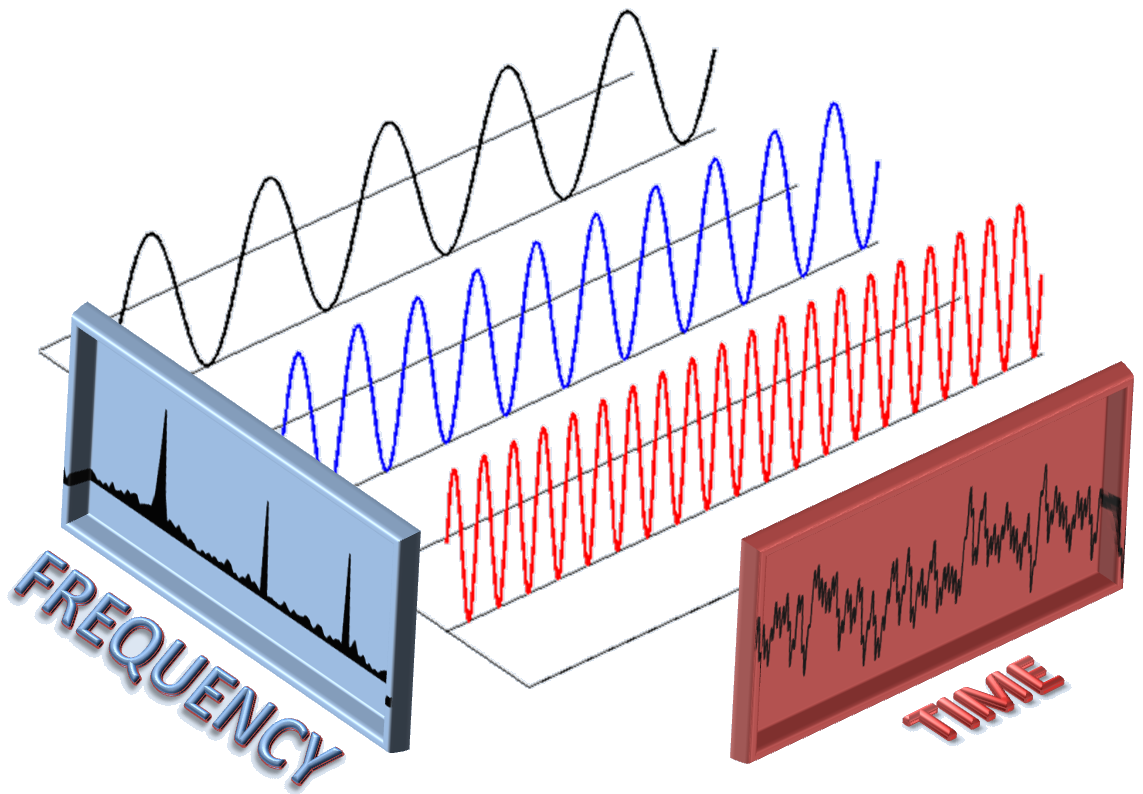
\includegraphics[scale=0.4]{title2.png}
		
		\vfill
		
		{\large \monthyear\today}
		
	\end{center}
\end{titlepage}

	\tableofcontents
	\listoffigures
	\lstlistoflistings
	\cleardoublepage \pagenumbering{arabic}
	
	\chapter{Errori ed aritmetica finita}
	\label{chapterErroriAritmeticaFinita}
	\pagenumbering{arabic}
	\minitoc \mtcskip
	\lettrine{Q}{}uando si utilizza un metodo numerico per risolvere un problema matematico non sempre si ottiene un \textbf{risultato esatto}, ma un \textbf{risultato approssimato}, che differisce dal risultato esatto.\\
	Sia $x \in \mathbb{R}$ il risultato esatto e $\tilde{x}$ il risultato approssimato corrispondente \begin{defi}
		La quantit�
		$$ \Delta x \equiv \tilde{x} - x $$
		rappresenta l'\textbf{errore assoluto} commesso.
	\end{defi}
	Tuttavia questa quantit� non � un buon indice di valutazione dell'errore, in quanto l'errore non viene in alcun modo rapportato all'ordine di grandezza del risultato: un errore assoluto pari a $10^{-3}$ rappresenta un errore trascurabile se, ad esempio, $x = 10^{8}$ ma allo stesso tempo � un errore enorme per $x = 10^{-3}$.\\
	Per poter meglio valutare il ``peso'' che l'errore ha sul risultato approssimato viene quindi introdotto un nuovo concetto
	\begin{defi}
		Se $x \neq 0$, si dice \textbf{errore relativo} la quantit�
		$$\varepsilon_x \equiv \dfrac{\Delta x}{x} = \dfrac{\tilde{x} - x}{x}$$
	\end{defi}
	Spesso l'errore relativo viene rapportato ad 1: valori di $\varepsilon_x$ vicini a 0 significano un errore ``piccolo'', mentre un errore relativo pari ad 1 implica una perdita totale di informazione.\\	
	Le cause che portano al verificarsi di tale errore sul risultato sono principalmente tre:
	\begin{itemize}
		\item errori di discretizzazione, o troncamento;
		\item errori di convergenza;
		\item errori di \textit{round-off}.
	\end{itemize}
	
	\section{Errori di discretizzazione}
		Si ha un errore di \textbf{discretizzazione}, o di \textbf{troncamento}, quando il problema dato viene formulato nel continuo e, per poter definire un metodo numerico che lo risolva eseguibile su calcolatore, � necessario sostituire tale problema con uno discreto che lo approssimi.
		
	\section{Errori di convergenza}
		\label{sez1.2}
		Se un metodo numerico utilizza una \textbf{funzione d'iterazione} $\Phi (x)$, allora si dice che il metodo � di tipo \textbf{iterativo}: esso non fornisce direttamente la soluzione al problema, ma genera una successione di risultati intermedi $\{x_n\}$, definita da
		\begin{equation}\label{iter}x_{n+1} = \Phi (x_n),\quad n=0, 1, 2, \dots,\end{equation}
		con $x_0$ \textit{approssimazione iniziale} fissata, che converge alla soluzione $x^*$, ovvero
		\begin{equation}\label{conv}\lim_{x \to +\infty} x_n = x^*.\end{equation}
		� ovvio per� che un calcolatore non pu� eseguire infinite iterazioni, quindi sar� necessario definire un opportuno \textbf{criterio d'arresto}.
		\begin{defi}
			Se l'iterazione (\ref{iter}) viene arrestata a $n = N - 1$, utilizzando come risultato $x_N$ al posto di $x^*$, la quantit�
			$$x_N - x^*$$
			viene detta \textbf{errore assoluto di convergenza}.
		\end{defi}
		
	\section{Errori di \textit{round-off}}
		Si ha un \textbf{errore di round-off}, e pi� precisamente \textbf{di rappresentazione}, quando si tenta di rappresentare una quantit� numerica, che spesso ha bisogno di una quantit� infinita di informazione per essere rappresentata esattamente (come ad esempio i numeri irrazionali), su un calcolatore, che per forza di cose � costretto ad utilizzare un'\textit{aritmetica finita}.\\
		Quindi qualunque numero, in un calcolatore, viene rappresentato mediante una quantit� finita di informazione, dando luogo, appunto, agli \textit{errori di rappresentazione}.\\
		In un calcolatore, inoltre, ogni numero viene rappresentato utilizzando una \textit{notazione posizionale} che utilizza le potenza di una base fissata $b \in \mathbb{N}$, con $b \geq 2$.\\
		Quando si parla di \textit{errore di rappresentazione} si distinguono due casi:
		\begin{itemize}
			\item numeri interi;
			\item numeri reali.
		\end{itemize}
		
		\subsection{Numeri interi}
			Un numero intero viene rappresentato, con base $b \in \mathbb{N}$, mediante una stringa del tipo
			$$\alpha_0\alpha_1\dots\alpha_N,$$
			con
			$$\alpha_0 \in \{+, -\},\quad \alpha_i \in \{0,1,\dots,b-1\},\quad i=1,\dots,N.$$
			Questa stringa corrisponde al numero
			$$
				n =
				\begin{cases}
					\sum_{i=1}^{N}\alpha_ib^{N-i}, & \quad \text{se $\alpha_0=+$},\\
					\sum_{i=1}^{N}\alpha_ib^{N-i} - b^N, & \quad \text{se $\alpha_0=-$}.
				\end{cases}
			$$
			Quindi risulta che l'insieme dei numeri correttamente rappresentabili tramite questa rappresentazione �
			$$[-b^N, b^N -1].$$
			
		\subsection{Numeri reali}
			Fissata una base $b \in \mathbb{N}$, un numero reale viene rappresentato mediante una stringa del tipo
			\begin{equation}\label{stringaReale}\alpha_0\alpha_1\dots\alpha_m\beta_1\dots\beta_s,\end{equation}
			dove
			\begin{equation}\label{condStringaReale}\alpha_0 \in \{+,-\},\quad\alpha_i,\beta_j\in\{0,1,\dots,b-1\},\quad i=1,\dots,m,\quad j=1,\dots,s,\end{equation}
			e tale che
			$$\alpha_1 \neq 0,$$
			cio� tale che il numero sia normalizzato. Questa rappresentazione viene detta \textbf{rappresentazione scientifica normalizzata} in base \textit{b}.\\
			Fissato lo \textbf{shift} $\nu\in\mathbb{N}$, la stringa (\ref{stringaReale}) rappresenta il numero
			\begin{equation}
				\label{numReale}
				r = 
				\begin{cases}
					\rho b^{\eta} & \quad \text{se $\alpha_0 = +$,}\\
					-\rho b^{\eta} & \quad \text{se $\alpha_0 = -$.}
				\end{cases}
			\end{equation}
			dove $\rho$ e $\eta$, rispettivamente \textbf{mantissa} ed \textbf{esponente}, sono le quantit�
			$$\rho=\pm\sum_{i=1}^{m}\alpha_ib^{1-i},\qquad \eta=\left(\sum_{j=1}^{s}\beta_jb^{s-j}\right) -\nu.$$
			Talvolta viene chiamato esponente anche la sola quantit� $e=\sum_{j=1}^{s}\beta_jb^{s-j}$, ovvero la quantit� tale che $\eta=e-\nu$.
			\begin{defi}
				L'\textbf{insieme dei numeri di macchina}, o numeri \textit{floating-point}, � definito come
				$$\mathcal{M}=\{0\}\cup\{\text{numeri della forma (\ref{stringaReale})}\}.$$
			\end{defi}
			\begin{teo}
				\label{teor1.1}
				$\mathcal{M}$ ha un numero finito di elementi.
			\end{teo}
			\begin{teo}
				Per ogni numero reale della forma (\ref{numReale}) vale
				$$1\leq |\rho| < b.$$
			\end{teo}
			\begin{teo}
				\label{teor1.3}
				Il pi� piccolo ed il pi� grande (in valore assoluto), tra i numeri di macchina diversi da 0, sono rispettivamente dati da:
				\begin{align}
					\label{rMinMax}
					&r_{min}=b^{-\nu},\\
					&r_{max}=(1-b^{-m})b^{\varphi},\quad \varphi=b^s-\nu.
				\end{align}
			\end{teo}
			Solitamente lo \textit{shift} $\nu$ viene scelto in modo che $r_{min} \approx r_{max}^{-1}$, ovvero $\nu\approx\sfrac{b^s}{2}$.\\
			Risulta allora che i numeri di macchina appartengono all'insieme
			\begin{equation}\label{insI}\mathcal{I}=[-r_{max}, -r_{min}]\cup\{0\}\cup[r_{min}, r_{max}],\end{equation}
			che ha un numero infinito di elementi, mentre, per il Teorema \ref{teor1.1}, $\mathcal{M}$ ha un numero finito di elementi.\\
			Quindi si definisce una funzione
			$$fl:\mathcal{I}\rightarrow\mathcal{M},$$
			che associa numeri reali $x\in\mathcal{I}$ a numeri di macchina $fl(x)\in\mathcal{M}.$ Quando $x\neq fl(x)$ si commette un \textit{errore di rappresentazione}.\\
			Sia
			$$x=(\alpha_1.\alpha_2\dots\alpha_m\alpha_{m+1}\dots)b^{\eta}$$
			un elemento positivo di $\mathcal{I}$. � possibile rappresentare tale numero
			\begin{itemize}
				\item con troncamento
					$$fl(x)=(\alpha_1.\alpha_2\dots\alpha_m)b^{\eta};$$
				\item con arrotondamento
					$$fl(x)=(\alpha_1.\alpha_2\dots\alpha_{m-1}\tilde{\alpha}_m)b^{\eta},$$
					con
					$$
						\tilde{\alpha}_m =
						\begin{cases}
							\alpha_m, &\quad \text{se $\alpha_{m+1}<\sfrac{b}{2}$,}\\
							\alpha_m+1, &\quad \text{se $\alpha_{m+1}\geq\sfrac{b}{2}$,}
						\end{cases}
					$$
					con eventuali riporti sulle cifre precedenti alla \textit{m}-esima nel caso in cui $\tilde{\alpha}_m\geq b.$
			\end{itemize}
			Infine si impone che $fl(0)=0$ e che $fl(x)=-fl(-x)$, se $x\in\mathcal{I}$ ed $x<0$.
			\begin{teo}
				\label{teor1.4}
				Se $x\in\mathcal{I}$ e $x\neq 0$, allora
				$$fl(x)=x(1+\varepsilon_x),\quad |\varepsilon_x|\leq u,$$
				dove
				$$
					u =
					\begin{cases}
						b^{1-m}, &\quad \text{con troncamento},\\
						\dfrac{1}{2}b^{1-m}, &\quad \text{con arrotondamento}.
					\end{cases}
				$$
			\end{teo}
			\begin{defi}
				La quantit� \textit{u}, definita nel Teorema \ref{teor1.4}, � detta \textbf{precisione di macchina}.
			\end{defi}
			
		\subsection{\textit{Overflow} e \textit{Underflow}}
			Quando si cerca di rappresentare un numero reale non contenuto nell'insieme $\mathcal{I}$ definito nella (\ref{insI}) si incorre in particolari tipi di errori:
			\begin{itemize}
				\item se $|x|>r_{max}$\\
					allora l'errore viene chiamato \textbf{overflow} e spesso viene risolto rappresentando i numeri pi� alti in valore assoluto di $r_{max}$ come una quantit� infinita.
				\item se $0<|x|<r_{min}$\\
					si incorre in una condizione d'errore denominata di \textbf{underflow}. Si pu� risolvere o con la tecnica di \textbf{store 0}, che prevede di rappresentare questi numeri con uno 0, o con la tecnica denominata \textbf{gradual underflow}, che consiste nel denormalizzare la mantissa, includendo quindi nell'insieme $\mathcal{M}$ anche i \textit{numeri di macchina denormalizzati}.
			\end{itemize}
			Riassumendo l'implementazione della funzione $fl$ si ha che
			$$
				fl(x)=
				\begin{cases}
					0,&\quad \text{se $x=0$,}\\
					\tilde{x}\equiv x(1+\varepsilon_x),\quad |\varepsilon_x|\leq u,&\quad \text{se $r_{min}\leq |x|\leq r_{max}$,}\\
					underflow,&\quad \text{se $0<|x|<r_{min}$,}\\
					overflow,&\quad \text{se $|x|>r_{max}$.}
				\end{cases}
			$$
			
		\subsection{Lo standard IEEE 754}
			\label{subSec1.3.4}
			Lo standard per la rappresentazione di numeri reali pi� diffuso � l'\textit{IEEE 754}, che utilizza una reppresentazione in base $b=2$ ed utilizza una tecnica di arrotondamento definita \textbf{round to even}, ovvero rappresentando $fl(x)$ come il numero di macchina ``pi� vicino'' ad $x$ (nel caso vi fossero due numeri reali equidistanti viene scelto quello il cui ultimo bit della mantissa � \textit{pari}, ossia 0).\\
			Con questo standard viene guadagnato un bit della mantissa in quanto essa sar� sempre della forma $1.f$, per numeri normalizzati, o della forma $0.f$ per numeri denormalizzati. pertanto viene memorizzata soltanto la \textit{frazione} $f$.\\
			Lo standard si suddivide in due formati: \textit{singola precisione} e \textit{doppia precisione}.\\
			Di seguito � riportato il numero di bit assegnato a ciascun formato\\
			\begin{center}
				\begin{tabular}{c||c|c}
					& Singola precisione & Doppia precisione\\
					\hline
					segno & 1 & 1\\
					\hline
					frazione (mantissa) & 23 (24) & 52 (53)\\
					\hline
					esponente & 8 & 11\\
					\hline
					totale & 32 & 64\\
					\hline
				\end{tabular}
			\end{center}
			Mentre per quanto riguarda l'implementazione dei due formati si ha la seguente tabella:
			\begin{center}
				\begin{tabular}{|c|c|c|}
					\hline
					Singola & Doppia & \multirow{2}{*}{Interpretazione}\\
					precisione & precisione &\\
					\hline
					\multirow{2}{*}{$0<e<255$} & \multirow{2}{*}{$0<e<2047$} & mantissa normalizzata\\
					& & ($\nu=127$ in singola precisione, $\nu=1023$ in doppia)\\
					\hline
					\multicolumn{2}{|c|}{\multirow{2}{*}{$e=0$ e $f\neq 0$}} & mantissa denormalizzata\\
					\multicolumn{2}{|c|}{} & ($\nu=126$ in singola precisione, $\nu=1022$ in doppia)\\
					\hline
					\multicolumn{2}{|c|}{\multirow{2}{*}{$e=f=0$}} & zero\\
					\multicolumn{2}{|c|}{} & (con segno)\\
					\hline
					\multicolumn{2}{|c|}{$f=0$} & infinito\\
					$e=255$ & $e=2047$ & (con segno)\\
					\hline
					\multicolumn{2}{|c|}{$f\neq 0$} & NaN\\
					$e=255$ & $e=2047$ & (Not a Number)\\
					\hline
				\end{tabular}
			\end{center}
			
		\subsection{Aritmetica finita}
			Quando si eseguono delle operazioni in aritmetica finita si deve tenere conto dell'insieme di rappresentabilit�.\\
			Per quanto riguarda i numeri interi, se entrambi gli operandi ricadono nell'insieme di rappresentabilit�, allora l'implementazione non differisce dalla corrispettiva operazione algebrica.\\
			Se invece si sta operando con numeri reali, allora si deve tener conto che l'implementazione opera tra numeri di macchina e restituisce un numero di macchina come risultato.\\
			Ad esempio l'implementazione della somma algebrica in aritmetica finita sar�:
			\begin{equation}\label{sommaAF}x\oplus y = fl(fl(x) + fl(y),\quad x,y\in\mathbb{R}.\end{equation}
			Ovviamente, in questo secondo caso, propriet� come associativit� o distributivit� possono non valere pi�.\\
			
		\subsection{Conversione tra tipi diversi}
			Spesso capita di dover convertire un numero intero in un reale e viceversa. La conversione da intero a reale � sempre possibile, introducendo al pi� un errore dell'ordine di $u$, se il numero di bit della mantissa non bastano a rappresentare il numero (a parit� di bit nella rappresentazione come intero e come reale si ha che la mantissa ha meno bit a disposizione rispetto alla rappresentazione come intero). La conversione da reale ad intero � invece, generalmente, pi� problematica, in quanto il numero che si vuole convertire potrebbe non appartenere all'insieme degli interi rappresentabili $\{-b^N,\dots ,b^N-1\}$, come ad esempio tutti i numeri con virgola.
		
	\section{Condizionamento di un problema}
		\label{sez1.4}
		Sia
		\begin{equation}\label{problDef}y=f(x)\end{equation}
		la formalizzazione di un problema matematico che vogliamo risolvere, con $x\in\mathbb{R}$ dati di ingresso, $f:\mathbb{R}\rightarrow\mathbb{R}$ funzione che descrive formalmente il problema ed $y\in\mathbb{R}$ soluzione del problema.\\
		Quando si decide di risolvere un problema del genere con un calcolatore viene definito un opportuno metodo numerico che risolva il problema in questione, ma di fatto il problema che ci troveremo a risolvere sar� del tipo
		$$\tilde{y}=\tilde{f}(\tilde{x}),$$
		dove $\tilde{x}$ rappresenta i dati in ingresso \textit{perturbati} (cio� con errori di \textit{round-off} o ottenuti sperimentalmente), $\tilde{f}$ indica che il metodo numerico � implementato in aritmetica finita (con eventuali errori di \textit{discretizzazione} o \textit{convergenza}) e $\tilde{y}$ denota i dati in uscita affetti dai precedenti errori.\\
		Ci� che � interessante studiare � il \textbf{condizionamento del problema}, ovvero come gli errori sui dati in ingresso $\varepsilon_x=\dfrac{\tilde{x}-x}{x}$ si propagano attraverso l'esecuzione del metodo numerico fino a definire l'errore $\varepsilon_y=\dfrac{\tilde{y}-y}{y}$ commesso sulla soluzione finale. Per un'analisi pi� approfondita e completa dell'errore del metodo numerico utilizzato si dovrebbero considerare anche gli errori introdotti dall'utilizzo di $\tilde{f}$ al posto di $f$, tuttavia, per semplicit�, ci limitiamo a studiare il problema
		$$\tilde{y}=f(\tilde{x}).$$
		Come accennato precedentemente, se si considerano gli errori relativi sui dati di ingresso e sulla soluzione finale si ha che
		$$\tilde{x}=x(1+\varepsilon_x),\quad\tilde{y}=y(1+\varepsilon_y).$$
		Ci� che ci interessa determinare �, quindi, la relazione che intercorre tra $\varepsilon_x$ e $\varepsilon_y$.\\
		Sviluppando $f(\tilde{x})$ in $x$ si ottiene
		$$f(\tilde{x})=f(x(1+\varepsilon_x))=f(x+x\varepsilon_x)=P_1(x+x\varepsilon_x;x)+O((x\varepsilon_x)^2)=f(x)+f'(x)x\varepsilon_x+O(\varepsilon_x^2),$$
		ovvero
		$$\tilde{y}=y-y\varepsilon_y = f(x)+f'(x)x\varepsilon_x+O(\varepsilon_x^2).$$
		Ricordando la (\ref{problDef}) e considerando un'\textit{analisi al primo ordine} (ovvero trascurando l'errore $O(\varepsilon_x^2)$), si ha che
		$$y+y\varepsilon_y\approx y+f'(x)x\varepsilon_x$$
		$$y\varepsilon_y\approx f'(x)x\varepsilon_x$$
		$$\varepsilon_y\approx f'(x)\dfrac{x}{y}\varepsilon_x$$
		$$|\varepsilon_y|\approx |f'(x)\dfrac{x}{y}|\cdot |\varepsilon_x| \equiv k|\varepsilon_x|.$$
		Quindi si ha che
		\begin{equation}\label{numCond}k \equiv |f'(x)\dfrac{x}{y}|.\end{equation}
		\begin{defi}
			Il \textit{fattore di amplificazione} $k$, che misura di quanto gli errori sui dati iniziali si possono amplificare sull'errore della soluzione finale, � detto \textbf{numero di condizionamento del problema} (\ref{problDef}).
		\end{defi}
		L'ordine di grandezza di $k$ determina quindi il condizionamento del problema:
		\begin{itemize}
			\item se $k\approx 1$, allora l'ordine degli errori finali � uguale a quello degli errori sui dati in ingresso ed il problema si dice \textbf{ben condizionato}.
			\item se $k\gg 1$ significa che nell'eseguire il metodo numerico gli errori finali risultano essere molto pi� grandi rispetto agli errori sui dati in ingresso. Il problema si dice in questo caso \textbf{malcondizionato}.
		\end{itemize}
		Se un problema risulta avere numero di condizionamento pari a $k\approx u^{-1}$, allora qualunque risultato sar� privo di significato: infatti l'errore sui dati di ingresso sar� dell'ordine di $u$, il che vuol dire che risulter� $\varepsilon_y=1$, che equivale ad una totale perdita di informazione. Se il problema risulta essere malcondizionato l'unica possibilit� per ottenere risultati accettabili � quella di riformulare il problema tentando di ottenere un condizionamento migliore; se invece il problema � ben condizionato si deve utilizzare un metodo numerico che risolva il problema mantenendone le buone propriet� di condizionamento (tali metodi numerici sono detti \textit{metodi numericamente stabili}).\\
		Analizziamo il condizionamento delle operazioni algebriche elementari:
		\begin{itemize}
			\item \textbf{\underline{Somma algebrica}}\\
				Il problema in questione �
				$$y=x_1+x_2,\qquad x_1,x_2\in\mathbb{R},\quad x_1+x_2\neq 0.$$
				Siano $\varepsilon_1$ e $\varepsilon_2$ gli errori sui dati in ingresso, si ha
				$$y(1+\varepsilon_y)=x_1(1+\varepsilon_1)+x_2(1+\varepsilon_2)=x_1+x_2+x_1\varepsilon_1+x_2\varepsilon_2.$$
				Si ottiene quindi
				$$y\varepsilon_y=x_1+x_2+x_1\varepsilon_1+x_2\varepsilon_2 -y$$
				$$y\varepsilon_y=x_1+x_2+x_1\varepsilon_1+x_2\varepsilon_2 -x_1-x_2$$
				$$|y\varepsilon_y|=|x_1\varepsilon_1+x_2\varepsilon_2|\leq |x_1\varepsilon_1|+|x_2\varepsilon_2|\leq (|x_1|+|x_2|)\varepsilon_x,\quad\varepsilon_x=max\{|\varepsilon_1|,|\varepsilon_2|\}$$
				\begin{equation}\label{condSomma}|\varepsilon_y|\leq\dfrac{|x_1|+|x_2|}{|y|}\varepsilon_x=\dfrac{|x_1|+|x_2|}{|x_1+x_2|}\varepsilon_x.\end{equation}
				Quindi risulta che
				$$k\leq\dfrac{|x_1|+|x_2|}{|x_1+x_2|}.$$
				Detto questo si possono avere due casi:
				\begin{itemize}
					\item $x_1x_2>0$: se gli addendi sono concordi, allora $k=1$ e la somma � ben condizionata;
					\item $x_1\approx -x_2$: se invece gli addendi sono di segno opposto il numero di condizionamento $k$ pu� essere arbitrariamente grande, perci� in questo caso la somma � malcondizionata. Questo particolare malcondizionamento, in aritmetica finita, prende il nome di \textit{cancellazione numerica}.
				\end{itemize}
			\item \textbf{\underline{Moltiplicazione}}\\
				Il problema della moltiplicazione di due numeri reali � formulato come segue:
				$$y=x_1x_2,\qquad x_1,x_2\in\mathbb{R},\quad x_1x_2\neq 0$$
				Introducendo gli errori relativi
				$$y(1+\varepsilon_y)=x_1(1+\varepsilon_1)x_2(1+\varepsilon_2)=x_1x_2(1+\varepsilon_1+\varepsilon_2+\varepsilon_1\varepsilon_2).$$
				Trascurando il termine quadratico si ha che
				\begin{align*}
					y\varepsilon_y&\approx x_1x_2(1+\varepsilon_1+\varepsilon_2)-y=\\
					&=x_1x_2(1+\varepsilon_1+\varepsilon_2)-x_1x_2=\\
					&=x_1x_2(\varepsilon_1+\varepsilon_2)
				\end{align*}
				$$\varepsilon_y\approx\dfrac{x_1x_2(\varepsilon_1+\varepsilon_2)}{x_1x_2}=\varepsilon_1+\varepsilon_2$$
				$$|\varepsilon_y|\approx |\varepsilon_1+\varepsilon_2|\leq 2\varepsilon_x,\qquad \varepsilon_x=\{|\varepsilon_1|, |\varepsilon_2|\}.$$
				Quindi il numero di condizionamento risulta essere $k=2$, pertanto la moltiplicazione � sempre ben condizionata.
			\item \textbf{\underline{Divisione}}\\
				Esaminiamo adesso il problema
				$$y=\dfrac{x_1}{x_2},\qquad x_1,x_2\in\mathbb{R},\quad x_1x_2\neq 0.$$
				Si ha che
				\begin{align*}
					y(1+\varepsilon_y)&=\dfrac{x_1(1+\varepsilon_1)}{x_2(1+\varepsilon_2)}=\dfrac{x_1}{x_2}\cdot\dfrac{(1+\varepsilon_1)(1-\varepsilon_2)}{(1+\varepsilon_2)(1-\varepsilon_2)}=\dfrac{x_1}{x_2}\cdot\dfrac{(1+\varepsilon_1)(1-\varepsilon_2)}{(1-\varepsilon_2^2)}\approx\\
					&\approx \dfrac{x_1}{x_2}(1+\varepsilon_1)(1-\varepsilon_2)=\dfrac{x_1}{x_2}(1+\varepsilon_1-\varepsilon_2-\varepsilon_1\varepsilon_2),
				\end{align*}
				dove l'approssimazione � dovuta al fatto che si � trascurato il termine quadratico $\varepsilon_2^2$.\\
				Trascurando anche il termine quadratico $\varepsilon_1\varepsilon_2$ si ottiene quindi
				$$y\varepsilon_y\approx\dfrac{x_1}{x_2}(1+\varepsilon_1-\varepsilon_2)-y$$
				$$y\varepsilon_y\approx\dfrac{x_1}{x_2}(1+\varepsilon_1-\varepsilon_2)-\dfrac{x_1}{x_2}$$
				$$\varepsilon_y\approx\dfrac{x_1}{x_2}(\varepsilon_1-\varepsilon_2)\cdot\dfrac{x_2}{x_1}$$
				$$\varepsilon_y\approx\varepsilon_1-\varepsilon_2$$
				$$|\varepsilon_y|\approx|\varepsilon_1-\varepsilon_2|\leq 2\varepsilon_x,\qquad\varepsilon_x=\{|\varepsilon_1|,|\varepsilon_2|\}.$$
				Anche in questo caso il numero di condizionamento del problema risulta essere $k=2$, quindi la divisione, come la moltiplicazione, � sempre ben condizionata.
		\end{itemize}
		
	\section*{Esercizi}
		\addcontentsline{toc}{section}{Esercizi}
		\markboth{\textsc{\uppercase{Capitolo }\ref{chapterErroriAritmeticaFinita}\uppercase{. Errori ed aritmetica finita}}}{\textsc{\uppercase{Esercizi}}}
		\begin{es} %1.1
			\label{es:1.1}
			Sia $x = \pi \approx 3.1415 = \tilde{x}$. Calcolare il corrispondente errore relativo $\varepsilon_x$. Verificare che il numero di cifre decimali corrette nella rappresentazione approssimata di $x$ mediante $\tilde{x}$ � all'incirca dato da
			$$-\log_{10} |\varepsilon_x|.$$
		\end{es}
		\begin{sol}
			Per definizione di errore relativo si ha che
			$$\varepsilon_x = \dfrac{\tilde{x} - x}{x} = \dfrac{3.1415 - \pi}{pi} \approx -2.9493 \times 10^{-5}$$
			Risulta allora che $-\log_{10}|\varepsilon_x| \approx 4.5303$; infatti 4 � il numero di cifre decimali esatte di 3.1415 come approssimazione di $\pi$ in quanto l'errore assoluto
			$$\Delta x = \tilde{x} - x = 3.1415 - \pi \approx -9.2654 \times 10^{-5}$$
			risulta essere dell'ordine di $10^{-5}$, ovvero ha le prime 4 cifre decimali pari a zero.
			\begin{flushright}
				\underline{Riferimenti \textsc{Matlab}}\\
				Codice \ref{lst:es1.1} (pagina \pageref{lst:es1.1})
			\end{flushright}
		\end{sol}
		\sectionline
		\begin{es} %1.2
			Dimostrare che, se $f(x)$ � sufficientemente regolare e $h > 0$ � una quantit� ``piccola'', allora:
			$$\dfrac{f(x_0 + h) - f(x_0 - h)}{2h} = f'(x_0) + O(h^2),$$
			$$\dfrac{f(x_0 + h) -2f(x_0) + f(x_0 - h)}{h^2} = f''(x_0) + O(h^2).$$
		\end{es}
		\begin{sol}
			Per queste due dimostrazioni si deve sviluppare la funzione $f(x)$ mediante un polinomio di Taylor di grado opportuno. Ricordiamo che lo sviluppo in polinomio di Taylor di grado \textit{n} della funzione $f(x)$ centrato in $x_0$ � $P_n(x; x_0) = \sum_{k=0}^{n} \dfrac{(x - x_0)^k}{k!}f^{(k})(x_0)$ e che il resto \textit{n}-esimo vale $R_n(x; x_0) = O(x - x_0)^{n+1}$.\\
			Per la prima uguaglianza si sviluppa $f(x)$ nel polinomio di Taylor al secondo ordine
			\begin{align*}
				f(x) &= P_2(x;x_0)+R_2(x;x_0)=\\
				&=f(x_0) + (x - x_0)f'(x_0) + \dfrac{(x - x_0)^2}{2}f''(x_0) + O((x - x_0)^3).
			\end{align*}
			Calcolando questo sviluppo in $x = (x_0 + h)$ e $x = (x_0 - h)$ si ottiene
			$$f(x_0 + h) = f(x_0) +hf'(x_0) + \dfrac{h^2}{2}f''(x_0) + O(h^3),$$
			$$f(x_0 - h) = f(x_0) -hf'(x_0) + \dfrac{h^2}{2}f''(x_0) + O(h^3).$$
			Quindi sostituendo nel rapporto incrementale di partenza si ha che
			\begin{align*}
				\dfrac{f(x_0 + h) - f(x_0 - h)}{2h} &= \dfrac{f(x_0) + hf'(x_0) + \dfrac{h^2}{2}f''(x_0) + O(h^3)}{2h} +\\
				&-\dfrac{f(x_0) - hf'(x_0) + \dfrac{h^2}{2}f''(x_0) + O(h^3)}{2h} =\\
				&=\dfrac{2hf'(x_0) + o(h^3)}{2h} = f'(x_0) + O(h^2).
			\end{align*}
			Per la seconda uguaglianza � invece necessario utilizzare un'approssimazione con Taylor al terzo ordine
			\begin{align*}
			f(x) &= P_3(x;x_0)+R_3(x;x_0)=\\
			&=f(x_0) + (x - x_0)f'(x_0) + \dfrac{(x - x_0)^2}{2}f''(x_0) +\\
			&+ \dfrac{(x - x_0)^3}{6}f'''(x_0) + O((x - x_0)^4)
			\end{align*}
			e come prima si calcola tale sviluppo in $x = (x_0 + h)$ e $x = (x_0 - h)$
			$$f(x_0 + h) = f(x_0) + hf'(x_0) + \dfrac{h^2}{2}f''(x_0) + \dfrac{h^3}{6}f'''(x_0) + O(h^4),$$
			$$f(x_0 - h) = f(x_0) - hf'(x_0) + \dfrac{h^2}{2}f''(x_0) - \dfrac{h^3}{6}f'''(x_0) + O(h^4).$$
			Quindi sostituendo come nell'uguaglianza precedente si ottiene
			\begin{align*}
				\dfrac{f(x_0 + h) -2f(x_0) + f(x_0 - h)}{h^2} &= \dfrac{h^2f''(x_0) + O(h^4)}{h^2} =\\
				&= f''(x_0) + O(h^2).
			\end{align*}
		\end{sol}
		\sectionline
		\begin{es} %1.3
			\label{es:1.3}
			Dimostrare che il metodo iterativo (\ref{iter}), convergente a $x^*$ (vedi (\ref{conv})), deve verificare la condizione di consistenza
			$$x^* = \Phi (x^*).$$
			Ovvero, la soluzione cercata deve essere un \underline{punto fisso} per la funzione di iterazione che definisce il metodo.
		\end{es}
		\begin{sol}
			Essendo il metodo iterativo convergente, per definizione risulta che
			$$\lim_{x \to +\infty} x_n = x^*.$$
			Supponendo la funzione $\Phi (x_n)$ continua, si ha
			$$\lim_{n \to +\infty} \Phi (x_n) = \Phi (\lim_{n \to +\infty} x_n) = \Phi (x^*),$$
			inoltre, essendo per definizione $\Phi (x_n) = x_{n+1}$,
			$$\lim_{n \to +\infty} \Phi (x_n) = \lim_{x \to +\infty} x_{n+1} = x^*,$$
			da cui la tesi, $x^* = \Phi (x^*).$
		\end{sol}
		\sectionline
		\begin{es} %1.4
			\label{es:1.4}
			Il metodo iterativo
			$$x_{n+1} = \dfrac{x_nx_{n+1} +2}{x_n +x_{n-1}},\quad n=1, 2,\dots,\quad x_0=2, x_1=1.5,$$
			definisce una successione di approssimazioni convergente a $\sqrt{2}$. Calcolare a quale valore si \textit{n} bisogna arrestare l'iterazione, per avere un errore di convergenza $\approx 10^{-12}$. Comparare con i risultati nella seguente tabella
			\begin{center}
				\begin{tabular}{|c|l|}
					\hline
					\textit{n} & $x_n$\\
					\hline
					0 & $2$\\
					1 & $1.5$\\
					2 & $1.416666666666\dots$\\
					3 & $1.414215686274\dots$\\
					4 & $1.414213562374\dots$\\
					\hline
				\end{tabular}
			\end{center}
			relativa all'iterazione
			$$x_{n+1} = \dfrac{1}{2}\left(x_n + \dfrac{2}{x_n}\right),\quad n=0,1,2,\dots,\quad x_0=2.$$
			che approssima $\sqrt{2}.$
		\end{es}
		\begin{sol}
			Risulta che il primo metodo iterativo proposto (quello con i due punti iniziali $x_0$ ed $x_1$) approssima $\sqrt{2}$ con errore di convergenza assoluto dell'ordine di $10^{-12}$ per $i = 6$, come si pu� vedere dalla tabella seguente
			\begin{center}
				\begin{tabular}{c||l|l}
					\textit{i} & $x_i$ & $\Delta x$\\
					\hline
					0 & $2$ & $5.85786e-001$\\
					1 & $1.5$ & $8.57864e-002$\\
					2 & $1.428571428571\dots$ & $1.43578e-002$\\
					3 & $1.414634146341\dots$ & $4.20583e-004$\\
					4 & $1.414215686274\dots$ & $2.12390e-006$\\
					5 & $1.414213562688\dots$ & $3.15774e-010$\\
					6 & $1.414213562373\dots$ & $0$
				\end{tabular}
			\end{center}
			Per $i \geq 6$ l'errore riportato � 0, probabilmente a causa della precisione di macchina che non riesce a rappresentare numeri troppo ``piccoli''.\\
			Il secondo metodo proposto (quello con il solo punto iniziale $x_0 = 2$) risulta invece raggiungere un errore assoluto di convergenza per $i=4$.\\
			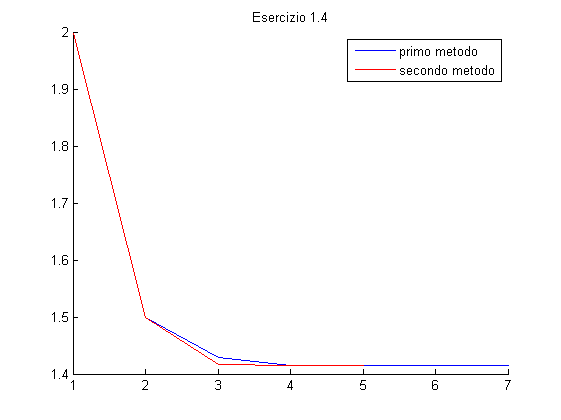
\includegraphics[width=0.8\textwidth]{es1_4.png}
			\begin{flushright}
				\underline{Riferimenti \textsc{Matlab}}\\
				Codice \ref{lst:es1.4} (pagina \pageref{lst:es1.4})
			\end{flushright}
		\end{sol}
		\sectionline
		\begin{es} %1.5
			Il codice Fortran
			\lstinputlisting[language=Fortran, frame=none, stepnumber=0, nolol=true]{code/fortran1_5.txt}
			produce il seguente output:
			\begin{center}
				\begin{tabular}{r r}
					1 & 32765\\
					2 & 32766\\
					3 & 32767\\
					4 & -32768\\
					5 & -32767\\
					6 & -32766\\
					7 & -32765\\
					8 & -32764\\
					9 & -32763\\
					10 & -32762
				\end{tabular}
			\end{center}
			Spiegarne il motivo.
		\end{es}
		\begin{sol}
			Essendo la variabile \textit{numero} di 2 byte significa che il bit pi� significativo ($\alpha_0$) rappresenta il segno (0 per un numero positivo ed 1 per un numero negativo), mentre i restanti 15 bit (da $\alpha_1$ ad $\alpha_15$) rappresentano il modulo del numero espresso in complemento a 2.\\
			Quando viene stampata la terza iterazione il numero vale 32767, ovvero
			$$\underbrace{0}_+\underbrace{111111111111111}_{32767},$$
			e ci si aspetta quindi che la quarta iterazione stampi il numero 32768. Tuttavia il numero 32768 avrebbe bisogno, per essere rappresentato in binario, di 16 bit per il modulo e di 1 per il segno, per un totale di 17. Infatti, eseguendo la somma in base due si ottiene
			$$\underbrace{1}_-\underbrace{000000000000000}_{32768},$$
			in quanto il riporto viene propagato fino al bit del segno.\\
			Successivamente il numero viene correttamente incrementato.
		\end{sol}
		\sectionline
		\begin{es} %1.6
			\label{es:1.6}
			Dimostrare i Teoremi \ref{teor1.1} e \ref{teor1.3}.
		\end{es}
		\begin{sol}
			\begin{itemize}
				\item \underline{Teorema \ref{teor1.1}}:\\
					Essendo l'insieme $\mathcal{M}$
					$$\mathcal{M}=\{0\}\cup\{\text{numeri della forma (\ref{stringaReale})}\},$$
					risulta che
					$$|\mathcal{M}|=|\{0\}|+|\{\text{numeri della forma (\ref{stringaReale})}\}|.$$
					Per la (\ref{condStringaReale}) si vede che:
					\begin{itemize}
						\item $\alpha_0$ pu� assumere 2 valori;
						\item $\alpha_1$ pu� assumere $b-1$ valori;
						\item $\alpha_i$, $\beta_j$ possono assumere \textit{b} valori, per $i=2,\dots,m$, $j=~1,\dots,s$.
					\end{itemize}
					Quindi la cardinalit� di $\mathcal{M}$ � data dalle disposizioni con ripetizione di questi elementi, ovvero
					$$|\mathcal{M}|=2(b-1)b^{m+s}+1<+\infty.$$
				\item \underline{Teorema \ref{teor1.3}}:\\
					Per quanto riguarda il minimo numero di macchina, positivo e diverso da 0, si ha che la mantissa minima vale $\rho_{min}=1$, mentre l'esponente minimo vale $\eta_{min}=0-\nu=-\nu$; quindi, applicando la (\ref{numReale})
					$$r_{min} = \rho_{min}b^{\eta_{min}} = 1\cdot b^{-\nu}=b^{-\nu}.$$
					Invece, per quanto riguarda $r_{max}$, si ha che la mantissa � massima quando tutti i suoi bit valgono $(b-1)$, ovvero
					\begin{align*}
						\rho_{max} &= (b-1)\sum_{i=1}^{m}b^{1-i} = (b-1)\sum_{k=0}^{m-1}b^{-k} =\\
						&=(b-1)\sum_{k=0}^{m-1}\left(\dfrac{1}{b}\right)^{k},
					\end{align*}
					ricordando che $\left(1-\dfrac{1}{b}\right)\sum_{k=0}^{m-1}\left(\dfrac{1}{b}\right)^k=1^m-\left(\dfrac{1}{b}\right)^m$, ovvero che $\sum_{k=0}^{m-1}\left(\dfrac{1}{b}\right)^k=b\dfrac{1-b^{-m}}{b-1}$, si ha che
					$$\rho_{max}=b\left(1-b^{-m}\right).$$
					Per quanto riguarda l'esponente massimo, risulta invece
					\begin{align*}
						\eta_{max}&=\left[(b-1)\sum_{i=1}^{s}b^{s-j}\right]-\nu=\left[(b-1)b^{s-1}\sum_{k=0}^{s-1}b^{-k}\right]-\nu=\\
						&=[b^s(1-b^{-s})]-\nu=(b^s-1)-\nu.
					\end{align*}
					Quindi, applicando di nuovo la (\ref{numReale}), si ottiene
					$$r_{max}=b\left(1-b^{-m}\right)b^{b^s-1-\nu} =\left(1-b^{-m}\right)b^{b^s-\nu}.$$
			\end{itemize}
		\end{sol}
		\sectionline
		\begin{es} %1.7
			Dimostrare il Teorema \ref{teor1.4} nel caso della rappresentazione con arrotondamento.
		\end{es}
		\begin{sol}
			Si distinguono i due casi in cui si ha arrotondamento per difetto e per eccesso:
			\begin{itemize}
				\item per difetto:\\
					In questo caso si ha che $\tilde{\alpha}_m=\alpha_m$ in quanto $\alpha_{m+1}<\sfrac{b}{2}$.
					\begin{align*}
						|\varepsilon_x|&=\dfrac{|x-fl(x)|}{|x|}=\dfrac{|(\alpha_1.\alpha_2\dots\alpha_m\alpha_{m+1}\dots-\alpha_1.\alpha_2\dots\tilde{\alpha}_m)b^{\eta}|}{|(\alpha_1.\alpha_2\dots)b^{\eta}|}=\\
						&=\dfrac{|0.\overbrace{0\dots0}^{m-1}\alpha_{m+1}\dots|}{|\alpha_1.\alpha_2\dots|},
					\end{align*}
					quindi, essendo il denominatore sicuramente $\geq 1$, il reciproco sar� sicuramente $\leq 1$. Se poi si trasla il numeratore di $m$ posizioni otteniamo
					$$|\varepsilon_x|\leq|(\alpha_{m+1}.\alpha_{m+2}\dots)b^{-m}|<\dfrac{b}{2}b^{-m}=\dfrac{1}{2}b^{1-m}\equiv u.$$
				\item per eccesso:\\
					In questo caso invece risulta che $\tilde{\alpha}_m=\alpha_m+1$, essendo $\alpha_{m+1}\geq\sfrac{b}{2}$.
					\begin{align*}
						|\varepsilon_x|&=\dfrac{|x-fl(x)|}{|x|}=\dfrac{|(\alpha_1.\alpha_2\dots\alpha_m\alpha_{m+1}\dots-\alpha_1.\alpha_2\dots\tilde{\alpha}_m)b^{\eta}|}{|(\alpha_1.\alpha_2\dots)b^{\eta}|}=\\
						&=\dfrac{|0.\overbrace{0\dots0}^{m-1}\hat{\alpha}_{m+1}\dots|}{|\alpha_1.\alpha_2\dots|},
					\end{align*}
					con $\hat{\alpha}_{m+1}=\tilde{\alpha}_m0-\alpha_m\alpha_{m+1}\leq\sfrac{b}{2}$.\\
					In questo caso per� � possibile che il valore assoluto al numeratore, traslato di $m$ posizioni, sia $>\sfrac{b}{2}$, come ad esempio nel caso estremo in cui $\hat{\alpha}_{m+1}=\sfrac{b}{2}$ e tutte le cifre successive valgono $(b-1)$. Quando si verifica questo si nota, tuttavia, che dividendo tale quantit� per il valore assoluto al denominatore si ottiene sicuramente una quantit� $<\sfrac{b}{2}$.\\
					Quando invece il valore assoluto al numeratore (traslato di $m$ posizioni) risulta gi� essere $\leq\sfrac{b}{2}$ si procede come nel caso precedente per difetto.\\
					Quindi in ogni caso si ha che
					$$|\varepsilon_x|\leq\dfrac{b}{2}b^{-m}=\dfrac{1}{2}b^{1-m}\equiv u.$$
			\end{itemize}
		\end{sol}
		\sectionline
		\begin{es} %1.8
			\label{es:1.8}
			Quante cifre binarie sono utilizzate per rappresentare, mediante arrotondamento, la mantissa di un numero, sapendo che la precisione di macchina � $u\approx 4.66\cdot 10^{-10}$?
		\end{es}
		\begin{sol}
			Applicando il Teorema \ref{teor1.4} si ha che $u=\dfrac{1}{2}b^{1-m}$, ovvero che
			$$m=1-\log_b2u.$$
			Ponendo $b=2$ e $u=4.66\cdot 10^{-10}$ e arrotondando, eventualmente, per eccesso, risulta
			$$m=-\log_24.66\cdot 10^{-10}\approx 31.$$
			Quindi servono almeno 31 cifre binarie per la mantissa per avere una precisione di macchina non superiore a $4.66\cdot 10^{-10}$.
			\begin{flushright}
				\underline{Riferimenti \textsc{Matlab}}\\
				Codice \ref{lst:es1.8} (pagina \pageref{lst:es1.8})
			\end{flushright}
		\end{sol}
		\sectionline
		\begin{es} %1.9
			Dimostrare che, detta $u$ la precisione di macchina utilizzata,
			$$-\log_{10}u$$
			fornisce, approssimativamente, il numero di cifre decimali correttamente rappresentate nella mantissa.
		\end{es}
		\begin{sol}
			Studiamo separatamente i casi in cui la rappresentazione avviene tramite troncamento e tramite arrotondamento.\\
			\begin{itemize}
				\item con troncamento:\\
					Per il Teorema \ref{teor1.4}, posto $b=10$, si ha che
					$$u=10^{1-m}\Rightarrow \log_{10}u=1-m\Rightarrow m=1-\log_{10}u\approx -\log_{10}u.$$
				\item con arrotondamento:\\
					Sempre per il Teorema \ref{teor1.4}, con $b=10$,
					\begin{align*}
						u&=\dfrac{1}{2}10^{1-m}\Rightarrow\log_{10}2u=1-m\Rightarrow\\
						&
						\begin{aligned}
							\Rightarrow m&=1-\log_{10}2u=1-\log_{10}2-\log_{10}u=\\
							&=\log_{10}5-\log_{10}u\approx -\log_{10}u.
						\end{aligned}
					\end{align*}
			\end{itemize}
		\end{sol}
		\sectionline
		\begin{es} %1.10
			\label{es:1.10}
			Con riferimento allo standard \textit{IEEE 754} (vedi Sezione \ref{subSec1.3.4}) determinare, relativamente alla doppia precisione:
			\begin{enumerate}
				\item il pi� grande numero di macchina,
				\item il pi� piccolo numero di macchina normalizzato positivo,
				\item il pi� piccolo numero di macchina denormalizzato positivo,
				\item la precisione di macchina.
			\end{enumerate}
			Confrontare le risposte ai primi due quesiti col risultato fornito dalle function \textsc{Matlab} \lstinline{realmax} e \lstinline{realmin}.
		\end{es}
		\begin{sol}
			\begin{enumerate}
				\item Si ha che il pi� grande numero di macchina in doppia precisione � dato dalla mantissa massima e l'esponente massimo. Per l'Esercizio \ref{es:1.6} si ha che $\rho=b(1-b^{-m})=2(1-2^{-53})=2-2^{-52}$, mentre $\eta=2046-\nu=2046-1023=1023$, essendo il valore $e=2047$ riservato.\\
					Quindi il massimo numero di macchina risulta essere
					$$r_{max}=(2-2^{-52})2^{1023}\approx 1.8\cdot 10^{308},$$
					infatti la function \lstinline{realmax} di \textsc{Matlab} restituisce lo stesso risultato.
				\item Per quanto riguarda il pi� piccolo numero di macchina normalizzato positivo basta applicare la (\ref{rMinMax}), con l'accortezza che l'esponente $e=0$ � riservato e quindi il pi� piccolo esponente risulta essere $e=1$:
					$$r_{minN}=2^{1-\nu}=2^{1-1023}=2^{-1022}\approx 2.2\cdot 10^{-308}.$$
					Utilizzando la function \textsc{Matlab} \lstinline{realmin} si perviene allo stesso risultato.
				\item Il pi� piccolo numero di macchina denormalizzato positivo � caratterizzato, per definizione, dall'esponente $e=0$ e dalla mantissa minima diversa da 0, ovvero la mantissa che ha tutti i bit, tranne il meno significativo, a 0, che vale $\rho=2^{-52}$.\\
					Quindi
					$$r_{minD}=2^{-52}2^{0-\nu}=2^{-52}2^{-1022}\approx 4.9\cdot 10^{-324}.$$
				\item Dal momento che lo standard \textit{IEEE 754} utilizza la rappresentazione con arrotondamento, per il Teorema \ref{teor1.4} si ha
					$$u=\dfrac{1}{2}b^{1-m}=\dfrac{1}{2}2^{1-53}=2^{-53}\approx 1.1\cdot 10^{-16}.$$
			\end{enumerate}
			\begin{flushright}
				\underline{Riferimenti \textsc{Matlab}}\\
				Codice \ref{lst:es1.10} (pagina \pageref{lst:es1.10})
			\end{flushright}
		\end{sol}
		\sectionline
		\begin{es} %1.11
			\label{es:1.11}
			Eseguire le seguenti istruzioni \textsc{Matlab}:
			\lstinputlisting[frame=none, stepnumber=0, nolol=true]{code/matlab1_11.m}
			Spiegarne il (non) funzionamento.
		\end{es}
		\begin{sol}
			Si nota che la rappresentazione in binario di $0.1$ � infinita periodica, in particolare vale $0.0\overline{0011}$, in quanto la frazione corrispondente $\sfrac{1}{10}$ non ha soltanto 2 come fattore primo del denominatore.\\
			Il valore memorizzato nel calcolatore della variabile \textit{delta}, e quindi il valore di $x$ alla prima iterazione, risulta essere $1\underbrace{0011\dots 0011}_{12 volte}001$ per la mantissa, che ricordiamo dev'essere normalizzata, e $\eta=-4$, che corrisponde all'esponente $e=\nu+\eta=1023-4=1019=01111111011_{[2]}$. Questa quantit� vale esattamente
			\begin{align*}
				r=0.&099999999999999993859642133668346\\
				&539081847127121849822415277933499\\
				&7546040964300101522745446966427383,
			\end{align*}\\
			ed � quindi minore di $0.1$.\\
			Risulta quindi che alla decima iterazione il valore memorizzato di $x$ � $0.\underbrace{1\dots 1}_{52 volte}<1_{[10]}$ mentre all'undicesima si ha $x=1.0\underbrace{0011\dots 0011}_{12 volte}001>1_{[10]}$. Quindi $x$ non assume mai il valore 1 e di conseguenza il ciclo � infinito.\\
			Per far funzionare il codice si pu� utilizzare il comando \textsc{Matlab} \lstinline{eps}, che restituisce lo spazio presente tra i numeri di macchina, ovvero la precisione di macchina, come guardia per la terminazione del ciclo, imponendo che il ciclo termini quando \lstinline{abs(x-1)<=eps}, che corrisponde all'impostare una tolleranza come criterio d'arresto.
			\begin{flushright}
				\underline{Riferimenti \textsc{Matlab}}\\
				Codice \ref{lst:es1.11} (pagina \pageref{lst:es1.11})
			\end{flushright}
		\end{sol}
		\sectionline
		\begin{es} %1.12
			\label{es:1.12}
			Individuare l'algoritmo pi� efficace per calcolare, in aritmetica finita, l'espressione $\sqrt{x^2 + y^2}$.
		\end{es}
		\begin{sol}
			L'espressione risulta essere condizionata in quanto i due elevamenti a potenza si possono ricondurre a due moltiplicazioni ($x^2=x\cdot x$ e $y^2=y\cdot y$), che sono sempre ben condizionate (con $k=2$); la somma risulta essere tra addendi concordi (entrambi positivi), quindi anch'essa ben condizionata (con $k=1$); ed infine l'estrazione della radice quadrata risulta ben condizionata (con $k=\sfrac{1}{2}$).\\
			Il problema in cui si pu� incorrere quando si tenta di valutare quest'espressione in aritmetica finita � che si verifichi un \textit{overflow}: infatti se prendiamo, ad esempio, $x=10^{200}$ ed $y=10^{200}$ si ha che il risultato � $\sqrt{2}\cdot 10^{200}$ il quale, se si utilizza lo standard \textit{IEEE 754} con doppia precisione, rientra nell'insieme dei numeri di macchina, essendo il massimo numero di macchina rappresentabile con questo formato $\approx 1.8\cdot 10^{308}$ (vedi Esercizio \ref{es:1.10}). Tuttavia l'elevamento a potenza produce il valore $10^{400}$ che, non rientrando nell'insieme dei numeri di macchina, causa un \textit{overflow}.\\
			Se si suppone, senza perdita di generalit�, che $x>y$, una soluzione consiste nel portare fuori dalla radice l'ordine di grandezza di $x$
			$$\sqrt{x^2 + y^2}=\sqrt{x^2(1 +\dfrac{y^2}{x^2})}=|x|\sqrt{1+\left(\dfrac{y}{x}\right)^2}.$$
			In questo modo si ha che l'espressione � correttamente calcolata (utilizzando i valori precedenti) $\sqrt{2}\cdot 10^{200}$ anzich� \textit{Inf} e l'espressione rimane ben condizionata, in quanto la divisione � un'operazione sempre ben condizionata (con $k=2$).\\
			Per valori molto grandi di $x$ e molto piccoli di $y$ si pu� incorrere nel problema opposto, ovvero un \textit{underflow}. Tuttavia questo problema � considerato meno grave in quanto pu� essere risolto denormalizzando il numero in floating point.
			\begin{flushright}
				\underline{Riferimenti \textsc{Matlab}}\\
				Codice \ref{lst:es1.12} (pagina \pageref{lst:es1.12})
			\end{flushright}
		\end{sol}
		\sectionline
		\begin{es} %1.13
			Eseguire le seguenti istruzioni \textsc{Matlab}:
			\lstinputlisting[frame=none, stepnumber=0, nolol=true]{code/matlab1_13.m}
			Concludere che la somma algebrica non gode, in aritmetica finita, della propriet� associativa.
		\end{es}
		\begin{sol}
			Il comando \textsc{Matlab} \lstinline{eps}, senza argomenti, restituisce la distanza tra 1 ed il primo numero maggiore di 1 in doppia precisione, ovvero $2^{-52}\approx 2.22\cdot 10^{-16}$.\\
			Quando, nella prima espressione, il valore di \lstinline{eps} viene dimezzato e poi sommato ad 1, si ottiene un valore che � a met� tra 1 ed $1+eps$, ovvero un numero non rappresentabile con la doppia precisione, che viene quindi interpretato come 1. Questo passaggio provoca l'errore, in quanto viene persa una quantit� pari ad $\sfrac{eps}{2}$, restituendo come risultato 0.\\
			La seconda espressione, invece, viene valutata correttamente 1 in aritmetica finita in quanto, dando priorit� alla sottrazione $(1-1)$ si ha che il valore $\sfrac{eps}{2}$ viene correttamente moltiplicato per il suo reciproco, restituendo, appunto, 1.\\
			Da questo semplice esempio si evince che, in aritmetica finita, la somma algebrica non gode, in generale, della propriet� associativa.
		\end{sol}
		\sectionline
		\begin{es} %1.14
			Eseguire e discutere il risultato delle seguenti istruzioni \textsc{Matlab}:
			\lstinputlisting[frame=none, stepnumber=0, nolol=true]{code/matlab1_14.m}
		\end{es}
		\begin{sol}
			Le due espressioni sono algebricamente equivalenti (per la propriet� distributiva del prodotto rispetto alla sottrazione), tuttavia la valutazione della prima restituisce, correttamente, il valore 0, mentre la seconda da come risultato \textit{NaN}, che sta per \textit{Not a Number}.\\
			Questo � dovuto al fatto che mentre nella prima espressione viene subito calcolato il valore 0, che annuller� anche il secondo fattore della moltiplicazione, nella seconda espressione viene eseguita prima la moltiplicazione e poi la sottrazione. Risulta quindi che la valutazione di $10^{300}\cdot 10^{300}$ viene interpretata come \textit{Inf}, ovvero un valore infinito, in quanto il valore effettivo $10^{600}$ non � rappresentabile in doppia precisione (pi� precisamente si verificano due overflow). La sottrazione degenera quindi nella forma indeterminata $[\infty - \infty]$, restituendo \textit{NaN} come valore.\\
			Da questo esempio si pu� dedurre che, in aritmetica finita, non vale la propriet� distributiva del prodotto rispetto alla sottrazione (e ragionevolmente la propriet� distributiva in generale).
		\end{sol}
		\sectionline
		\begin{es} %1.15
			Eseguire l'analisi dell'errore (relativo), dei due seguenti algoritmi per calcolare la somma di tre numeri (vedi (\ref{sommaAF})):
			$$1)\quad (x\oplus y)\oplus z,\qquad 2)\quad x\oplus(y\oplus z).$$
		\end{es}
		\begin{sol}
			L'espressione in aritmetica esatta � equivalente nei due casi ed � data da $R = (x+y)+z = x+(y+z)=x+y+z$.
			\begin{itemize}
				\item
					Nel primo caso si ha che l'espressione in aritmetica finita � data da
					\begin{align*}
						F_1&=(x\oplus y)\oplus z=\\
						&=fl(fl(fl(fl(x)+fl(y)))+fl(z))=\\
						&=[(x(1+\varepsilon_x)+y(1+\varepsilon_y))(1+\varepsilon_A)+z(1+\varepsilon_z)](1+\varepsilon_B).
					\end{align*}
					Quindi l'errore relativo, tenendo conto che $u\geq u^2\geq u^3$, � dato da
					\begin{align*}
						\varepsilon_1&=\dfrac{F_1-R}{R}=\\
						&=[(x(1+\varepsilon_x)+y(1+\varepsilon_y))(1+\varepsilon_A)+z(1+\varepsilon_z)](1+\varepsilon_B)=\\
						&=\dfrac{x(1+\varepsilon_x)(1+\varepsilon_A)(1+\varepsilon_B) + y(1+\varepsilon_y)(1+\varepsilon_A)(1+\varepsilon_B)}{x+y+z}+\\
						&\quad +\dfrac{z(1+\varepsilon_z)(1+\varepsilon_B) -x-y-z}{x+y+z}\leq\\
						&\leq \dfrac{x(1+u)^3 + y(1+u)^3 + z(1+u)^2 -x-y-z}{x+y+z}=\\
						&=\dfrac{x(3u+3u^2+u^3) + y(3u+3u^2+u^3) +z(2u+u^2)}{x+y+z}\leq\\
						&\leq\dfrac{7ux+7uy+3uz}{x+y+z}=\\
						&=u\left(3+4\dfrac{x+y}{x+y+z}\right).
					\end{align*}
				\item
					Analogamente per il secondo caso si ha che l'espressione in aritmetica finita � data da
					\begin{align*}
						F_2&=x\oplus (y\oplus z)=\\
						&=[x(1+\varepsilon_x)+(y(1+\varepsilon_y)+z(1+\varepsilon_z))(1+\varepsilon_C)](1+\varepsilon_D),
					\end{align*}
					e quindi l'errore relativo corrispondente � dato da
					$$\varepsilon_2=\dfrac{F_2-R}{R}=u\left(3+4\dfrac{y+z}{x+y+z}\right).$$
			\end{itemize}
			Si nota che l'unico modo per far diminuire l'errore relativo � di diminuire il numeratore, ovvero la quantit� $(x+y)$, nel primo caso, e $y+z$ nel secondo. Quindi se ne deduce che, anche se in aritmetica esatta le due espressioni sono equivalenti, in aritmetica finita l'espressione migliore (ovvero quella che presenter� un minor errore sul risultato) sar� quella che somma per primi i due addendi con valore minore tra i tre presenti nell'espressione.
		\end{sol}
		\sectionline
		\begin{es} %1.16
			Dimostrare che il numero di condizionamento del problema del calcolo di $y=\sqrt{x}$ � $k=\sfrac{1}{2}$.
		\end{es}
		\begin{sol}
			Applicando la (\ref{numCond}), in questo caso specifico si ha $y=f(x)=\sqrt{x}$ ed $f'(x)=\dfrac{1}{2\sqrt{x}}$.\\
			Quindi risulta che
			$$k=\left|\dfrac{1}{2\sqrt{x}}\cdot\dfrac{x}{\sqrt{x}}\right|=\left|\dfrac{1}{2}\cdot\dfrac{x}{x}\right|=\dfrac{1}{2}.$$
			L'estrazione da radice quadrata risulta quindi essere sempre ben condizionata.
		\end{sol}
		\sectionline
		\begin{es}[Cancellazione Numerica] %1.17
			\label{es:1.17}
			Si supponga di dover calcolare l'espressione
			$$y=0.12345678-0.12341234\equiv 0.00004444,$$
			utilizzando una rappresentazione decimale con arrotondamento alla quarta cifra significativa. Comparare il risultato esatto con quello ottenuto in aritmetica finita, e determinare la perdita di cifre significative derivante dalla operazione effettuata. Verificare che questo risultato � in accordo con l'analisi di condizionamento (vedi (\ref{condSomma})).
		\end{es}
		\begin{sol}
			Il problema in questione � una somma algebrica con addendi discordi, in particolare
			$$x_1=0.12345678,\qquad x_2=-0.12341234,\qquad y=x_1+x_2=0.00004444.$$
			Arrotondando $x_1$ ed $x_2$ alla quarta cifra decimale si ottengono i dati di ingresso perturbati
			$$\tilde{x_1}=0.1235,\qquad\tilde{x_2}=-0.1234,$$
			e la corrispondente soluzione del problema in aritmetica finita � calcolata come somma dei due addendi perturbati
			$$\tilde{y}=\tilde{x_1}+\tilde{x_2}=0.0001.$$
			Calcoliamo adesso gli errori relativi
			$$\varepsilon_1=\dfrac{\tilde{x_1}-x_1}{x_1}=\dfrac{0.1235-0.12345678}{0.12345678}\approx 3.5\cdot 10^{-4}$$
			$$\varepsilon_2=\dfrac{\tilde{x_2}-x_2}{x_2}=\dfrac{-0.1234+0.12341234}{-0.12341234}\approx -9.9\cdot 10^{-5}$$
			$$\varepsilon_y=\dfrac{\tilde{y}-y}{y}=\dfrac{0.0001-0.00004444}{0.00004444}\approx 1.25.$$
			Risulta quindi che il risultato ottenuto � privo di significato in quanto l'errore relativo sulla soluzione maggiore di $1$ implica una perdita totale di informazione. Ne consegue che sono state perse tutte le cifre significative della soluzione.\\
			Applicando la (\ref{condSomma}) si ha che
			$$k=\dfrac{|x_1|+|x_2|}{|x_1+x_2|}=\dfrac{0.12345678+0.12341234}{0.00004444}\approx 5.6\cdot 10^{3}$$
			$$\varepsilon_x=max\{|\varepsilon_1|, |\varepsilon_2|\}=|\varepsilon_1|\approx 3.5\cdot 10^{-4}.$$
			Si vede quindi che, essendo il numero di condizionamento del problema $k\gg 1$, il problema risulta malcondizionato.\\
			Se si prova a moltiplicare l'errore relativo massimo sui dati di ingresso $\varepsilon_x$ per il fattore di amplificazione calcolato $k$, si ottiene una maggiorazione dell'errore relativo sulla soluzione, che non si discosta di molto dal valore effettivamente calcolato
			$$k\varepsilon_x\approx 5.6\cdot 10^{3}\cdot 3.5\cdot 10^{-4}\approx 1.9\approx 1.25 \approx \varepsilon_y.$$
			\begin{flushright}
				\underline{Riferimenti \textsc{Matlab}}\\
				Codice \ref{lst:es1.17} (pagina \pageref{lst:es1.17})
			\end{flushright}
		\end{sol}
		\sectionline
		\begin{es}[Cancellazione Numerica] %1.18
			\label{es:1.18}
			Eseguire le seguenti istruzioni in \textsc{Matlab}:
			\lstinputlisting[frame=none, stepnumber=0, nolol=true]{code/matlab1_18.m}
			Valutare l'errore relativo sui dati di ingresso e l'errore relativo sul risultato ottenuto.
		\end{es}
		\begin{sol}
			Essendo gli addendi discordi e circa uguali in modulo, si ha che il problema � malcondizionato. Infatti il numero di condizionamento del problema vale
			$$k=\dfrac{|a|+|-b|}{|a-b|}=\dfrac{0.1+0.099999999999}{0.000000000001}\approx 2\cdot 10^{11}.$$
			Se si considera che i dati in ingresso sono affetti da un errore relativo dell'ordine della precisione di macchina, ovvero $\varepsilon_x=u\approx 1.1\cdot 10^{-16}$ (con doppia precisione, vedi Esercizio \ref{es:1.10}), allora l'errore relativo sulla soluzione finale sar� dell'ordine di
			$$\varepsilon_y\approx k\varepsilon_x \approx 2\cdot 10^{11}\cdot 1.1\cdot 10^{-16}\approx 2.2\cdot 10^{-5}.$$
			Infatti si ha che eseguendo il codice \textsc{Matlab} proposto risultano corrette (cio� 0) soltanto le prime $5$ cifre della soluzione, come si evince anche dal fatto che
			$$\lceil-\log_{10}|\varepsilon_y|\rceil \approx\lceil -\log_{10}(2.2\cdot 10^{-5})\rceil = 5.$$
			\begin{flushright}
				\underline{Riferimenti \textsc{Matlab}}\\
				Codice \ref{lst:es1.18} (pagina \pageref{lst:es1.18})
			\end{flushright}
		\end{sol}
		
	\section*{Codice degli esercizi}
		\addcontentsline{toc}{section}{Codice degli esercizi}
		\markboth{\textsc{\uppercase{Capitolo }\ref{chapterErroriAritmeticaFinita}\uppercase{. Errori ed aritmetica finita}}}{\textsc{\uppercase{Codice degli esercizi}}}
		\lstinputlisting[caption={Esercizio \ref{es:1.1}.}, label=lst:es1.1]{code/es1_1.m}
		\sectionline
		\lstinputlisting[caption={Esercizio \ref{es:1.4}.}, label=lst:es1.4]{code/es1_4.m}
		\sectionline
		\lstinputlisting[caption={Esercizio \ref{es:1.8}.}, label=lst:es1.8]{code/es1_8.m}
		\sectionline
		\lstinputlisting[caption={Esercizio \ref{es:1.10}.}, label=lst:es1.10]{code/es1_10.m}
		\sectionline
		\lstinputlisting[caption={Esercizio \ref{es:1.11}.}, label=lst:es1.11]{code/es1_11.m}
		\sectionline
		\lstinputlisting[caption={Esercizio \ref{es:1.12}.}, label=lst:es1.12]{code/es1_12.m}
		\sectionline
		\lstinputlisting[caption={Esercizio \ref{es:1.17}.}, label=lst:es1.17]{code/es1_17.m}
		\sectionline
		\lstinputlisting[caption={Esercizio \ref{es:1.18}.}, label=lst:es1.18]{code/es1_18.m}
		
	\chapter{Radici di una equazione}
	\label{chap:radici}
	\minitoc \mtcskip
	\lettrine{I}{}n questo capitolo studieremo il problema del calcolo degli \textit{zeri} reali di una funzione, ovvero risolvere l'equazione
	\begin{equation}
		\label{eqRad}
		f(x)=0,\qquad x\in\mathbb{R},\quad f:\mathbb{R}\rightarrow\mathbb{R},
	\end{equation}
	determinandone le \textit{radici} reali.\\
	In generale, questo tipo di problema, o ammette un numero \textit{finito} di soluzioni, o non ammette \textit{alcuna} soluzione, oppure ammette un numero \textit{infinito} di soluzioni.\\
	Di seguito supporremo che la funzione ammetta almeno una radice reale, presupposto sempre verificato nel caso in cui la funzione risulti continua in un intervallo $[a,b]$ con $f(a)f(b)<0$, per il Teorema di Bolzano (o Teorema degli Zeri).
	\section{Il metodo di bisezione}
		Il metodo di bisezione, per il calcolo di un'approssimazione di una radice di una funzione, si basa sul \textit{Teorema di Bolzano} poc'anzi accennato. Si suppone quindi che la funzione $f(x)$ considerata sia continua in un intervallo $[a,b]$ e che $f(a)f(b)<0$: in questo caso si dice che l'intervallo $[a,b]$ costituisce un \textbf{intervallo di confidenza} per la radice dell'equazione (\ref{eqRad}).\\
		Se denotiamo con $x^*$ la radice ricercata, il miglior risultato che possiamo ottenere in un primo momento � di stimare che
		$$x^*\approx x_1\equiv \dfrac{a+b}{2},$$
		che corrisponde al punto medio dell'intervallo $[a,b]$. In questo modo si ha che l'errore commesso sar� maggiorato dalla semi-ampiezza dell'intervallo di confidenza, ovvero
		$$|x^* - x_1| \leq \dfrac{b-a}{2}.$$
		A questo punto, per quanto riguarda il punto appena calcolato $x_1$, ci possiamo trovare in tre situazioni distinte e mutuamente esclusive:
		\begin{itemize}
			\item $f(x_1)=0$: in questo caso (assai raro) si ha che il punto trovato � effettivamente uno zero della funzione e costituisce, quindi, una soluzione al problema;
			\item $f(a)f(x_1)<0$: il procedimento precedente viene ripetuto sul nuovo intervallo di confidenza $[a,x_1]$;
			\item $f(x_1)f(b)<0$: viene ripetuto il procedimento precedente sull'intervallo $[x_1, b]$.
		\end{itemize}
		Quindi si ha che, se non viene trovata la radice cercata, allora l'intervallo di confidenza viene dimezzato, reiterando il procedimento: per questo motivo questo metodo prende il nome di \textbf{Metodo di Bisezione}.\\
		Come qualsiasi metodo iterativo � necessario definire un opportuno criterio d'arresto: in un primo momento si potrebbe pensare di terminare l'esecuzione quando viene trovato un punto $x_i$ tale che $f(x_i)=0$, ma tale criterio d'arresto risulta molto inefficace in quanto molto probabilmente quella condizione, specialmente in aritmetica finita, non si verificher� mai.
	\section{Criteri di arresto e condizionamento}
		Spesso si ha che non interessa determinare esattamente la radice della (\ref{eqRad}), ma una sua approssimazione entro una certa tolleranza $tol_x$, ovvero determinare un punto $\tilde{x}$ tale che
		$$|x^* - \tilde{x}|\leq tol_x.$$
		Tuttavia, non conoscendo il valore della radice $x^*$, si deve utilizzare $tol_x$ come criterio d'arresto facendo una stima sul numero minimo di passi d'iterazione da eseguire per ottenere un errore sicuramente minore o uguale a $tol_x$.\\
		Ricordiamo che l'errore commesso al primo passo � maggiorato dalla semi-ampiezza dell'intervallo di confidenza, ovvero che
		$$|x^*-x_1|\leq\dfrac{b-a}{2}.$$
		Analogamente si ha che al passo $i$-esimo $x_i=\dfrac{a_i+b_1}{2}$, con $[a_i, b_i]$ intervallo di confidenza al passo $i$-esimo, e l'errore commesso � maggiorato da
		$$|x^*-x_i|\leq\dfrac{b_i-a_i}{2}=\dfrac{b_{i-1}-a_{i-1}}{2^2}=\dots=\dfrac{b-a}{2^i}.$$
		Quindi il numero di passi da eseguire per ottenere un errore sicuramente minore o uguale a $tol_x$ � dato da
		$$\dfrac{b-a}{2^{i}}\leq tol_x$$
		$$2^{i}\geq\dfrac{b-a}{tol_x}$$
		$$i\geq\lceil\log_2\dfrac{b-a}{tol_x}\rceil=\lceil\log_2(b-a)-\log_2tol_x\rceil$$
		$$i_{max}\equiv \lceil\log_2(b-a)-\log_2tol_x\rceil.$$
		Inserendo quindi un limite superiore al numero di passi che si pu� effettuare si ha che l'algoritmo che descrive il metodo di bisezione terminer� sempre (cosa che non veniva garantita con il semplice controllo $f(x_i)=0$). Tuttavia rimane il fatto che il controllo $f(x_i)=0$ spesso risulta, specialmente in aritmetica finita, inefficace. Si pu� pensare allora di sfruttare una certa tolleranza anche sul valore che la funzione assume in un determinato punto, ricordando che, essendo $f(x)$ continua ed essendo $f(x^*)=0$, in un opportuno intorno di $x^*$ si avr� che i valori della funzione risulteranno ``piccoli''.\\
		Pertanto si sostituir� il controllo $f(x_i)=0$ con un controllo del tipo $|f(x_i)|\leq tol_f$, dove $tol_f$ rappresenta la tolleranza sul valore della funzione scelta in modo tale che $|x_i-x^*|\leq tol_x$.
		Supponendo $f(x)\in C^{(1)}$, si sviluppa la funzione in $x^*$ (trascurando l'errore di ordine quadratico commesso)
		\begin{align*}
			f(x)&=P_1(x;x^*)+O((x-x^*)^2)=\\
			&=f(x^*)+(x-x^*)f'(x^*)+O((x-x^*)^2)\approx\\
			&\approx f'(x^*)(x-x^*),
		\end{align*}
		da cui segue che
		$$x-x^*\approx \dfrac{f(x)}{f'(x^*)}$$
		\begin{equation}\label{errBisez}|x-x^*|\approx \dfrac{|f(x)|}{|f'(x^*)|}.\end{equation}
		Quindi, per avere $|x-x*|\approx tol_x$, occorre utilizzare una tolleranza sulla $f(x)$ che vale circa
		$$tol_f\approx |f'(x^*)|\cdot tol_x.$$
		Quindi si ha che
		\begin{itemize}
			\item $tol_f\ll tol_x$, se $f'(x^*)\approx 0$;
			\item $tol_f\gg tol_x$, se $f'(x^*)\gg 1.$
		\end{itemize}
		Ovvero si ha che, fissata $tol_x$, tanto pi� grande sar� la derivata $|f'(x^*)|$, tanto pi� grande sar� l'intorno di $tol_f$ e quindi meno stringente $tol_f$ stessa; viceversa fissata $tol_f$, tanto pi� grande sar� $|f'(x^*)|$, tanto pi� piccolo sar� l'intervallo di confidenza definito dall'intorno di $tol_x$.\\
		Se al passo $i$-esimo si ha l'intervallo di confidenza $[a_i,b_i]$, un'approssimazione della derivata $f'(x^*)$ � data da
		$$f'(x^*)\approx \dfrac{f(b_i)-f(a_i)}{b_i-a_i}.$$
		Vediamo di seguito un'implementazione in \textsc{Matlab} del metodo di bisezione, utilizzando i criteri d'arresto appena enunciati:
		\lstinputlisting[caption={Metodo di bisezione.}]{code/bisezione.m}
		Un altro importante aspetto dell'analisi dei criteri d'arresto per il metodo di bisezione � il condizionamento della radice $x^*$. Se si interpreta nella (\ref{errBisez}) il valore $f(x)$ della funzione come perturbazione del valore nullo e $|x-x^*|$ l'errore commesso sulla soluzione finale del problema, allora tale perturbazione sui dati di ingresso risulta amplificata di un fattore
		$$k=\dfrac{1}{f'(x^*)}$$
		durante l'esecuzione del metodo.\\
		Se ne deduce che $k$ pu� essere definito come \textbf{numero di condizionamento della radice} $x^*$.
		\begin{defi}
			Una radice $x^*$ ha \textbf{molteplicit� esatta} $m\geq 1$, se
			$$f(x^*)=f'(x^*)=\dots =f^{(m-1)}(x^*)=0,\quad f^{(m)}(x^*)\neq 0.$$
			Se $m=1$ la radice si dice \textbf{semplice}; altrimenti, se $m\geq 2$, si dice \textbf{multipla}.
		\end{defi}
		Quindi si ha che il problema delle radici multiple � sempre malcondizionato in quanto, essendo $f'(x^*)=0$, risulta che $k$ assume un valore virtualmente infinito.\\
		Si ha, infine, che se $f(x)$ � sviluppabile in serie di Taylor in $x^*$ (radice di $f(x)$ di molteplicit� $m$), allora tale funzione si pu� scrivere come
		$$f(x)= (x-x^*)^m g(x),$$
		con $g(x)$ funzione ancora sviluppabile in serie di Taylor in $x^*$ e tale che $g(x^*)\neq 0$.
	\section{Ordine di convergenza}
		Supponendo di utilizzare un generico metodo iterativo per l'approssimazione di una radice $x^*$ dell'equazione (\ref{eqRad}), denotiamo con $x_i$ l'approssimazione fornita dal metodo al passo $i$-esimo e $e_i$ l'errore commesso corrispondente
		$$e_i\equiv x_i - x^*.$$
		Quindi, come visto nella Sezione \ref{sez1.2}, tale metodo si dir� \textit{convergente} se
		$$\lim_{i\to\infty}e_i=0.$$
		Ovviamente la convergenza � un requisito fondamentale per un metodo numerico iterativo, ma � interessante studiare anche la ``velocit�'' con la quale il metodo converge verso la soluzione.\\
		Ad esempio, come gi� osservato nelle sezioni precedenti, per il metodo di bisezione risulta che ad ogni passo d'iterazione l'errore viene dimezzato, infatti si pu� dimostrare che
		$$\lim_{i\to\infty}\dfrac{|e_{i+1}|}{|e_i|}=\dfrac{1}{2}.$$
		\begin{defi}
			Se per un certo metodo iterativo si ha che $p$ � il pi� grande valore reale per cui vale
			\begin{equation}\label{ordConv}\lim_{i\to\infty}\dfrac{|e_{i+1}|}{|e_i|^p}=p<\infty,\end{equation}
			allora si dice che il metodo ha \textbf{ordine di convergenza} $p$ con \textbf{costante asintotica dell'errore} pari a $c$.\\
			Nel caso di $p=1$ si parla di \textbf{convergenza lineare}, nel caso $p=2$ di \textbf{convergenza quadratica}, ecc.
		\end{defi}
		Quindi si ha che il metodo di bisezione ha ordine di convergenza lineare ($p=1$) con costante asintotica dell'errore $c=\sfrac{1}{2}$.\\
		L'ordine di convergenza $p$ pu� assumere anche valori non interi, anche se deve necessariamente risultare $p\geq 1$ affinch� il metodo converga.\\
		Si nota che, per $p=1$ ed $i$ sufficientemente grande, vale
		$$|e_{i+1}|\approx c|e_i|,$$
		$$|e_{i+k}|\approx c^k|e_i|,$$
		pertanto un metodo iterativo con $p=1$ converge se e solo se $0\leq c<1$.\\
		In generale si ha che tanto pi� elevato � il l'ordine di convergenza di un metodo iterativo, tanto pi� velocemente esso converger� verso una radice $x^*$.
	\section{Il metodo di Newton}
		Supponiamo di disporre di un'approssimazione iniziale $x_0$ della radice $x^*$. La retta tangente al grafico nel punto $(x_0, f(x_0))$ � data dall'equazione
		$$y=f(x_0)+f'(x_0)(x-x_0).$$
		La nuova approssimazione $x_1$ della radice $x^*$ � data dall'intersezione tra la suddetta retta tangente e la retta delle ascisse, ovvero
		$$0=f(x_0)+f'(x_0)(x_1-x_0)$$
		$$x_1f'(x_0)=x_0f'(x_0)-f(x_0)$$
		$$x_1=x_0-\dfrac{f(x_0)}{f'(x_0)},$$
		che � definita se $f'(x_0)\neq 0$.\\
		Quindi al passo $(i+1)$-esimo si ha che l'espressione funzionale del \textbf{metodo di Newton} �
		\begin{equation}\label{newton}x_{i+1}=x_i-\dfrac{f(x_i)}{f'(x_i)},\qquad i=0,1,2,\dots\end{equation}
		Quindi il metodo di Newton consiste nella risoluzione successiva di equazioni lineari: ovviamente nel caso in cui la $f(x)$ sia una funzione lineare, il metodo fornisce il risultato in un solo passo.\\
		Rispetto al metodo di bisezione, che richiedeva come requisito la sola continuit� della funzione, il metodo di Newton ne richiede anche la derivabilit�. Inoltre, ad ogni passo, oltre alla valutazione della $f(x_i)$ si deve calcolare anche la derivata prima $f'(x_i)$.\\
		Questi svantaggi del metodo di Newton rispetto al metodo di bisezione vengono tuttavia ripagati dall'ordine di convergenza del metodo di Newton: infatti vale
		\begin{teo}
			Se $f(x)$ � sufficientemente regolare (cio� $f\in C^{(1)}$), il metodo di Newton converge quadraticamente verso radici semplici.
		\end{teo}
		\begin{teo}
			\label{teo2.2}
			Se $f(x)$ � sufficientemente regolare, il metodo di Newton converge linearmente verso una radice di molteplicit� $m>1$, con costante asintotica dell'errore pari a $(m-1)/m$.
		\end{teo}

	\section{Convergenza locale}
		Studiamo adesso quali sono le condizioni \textit{necessarie} affinch� un metodo iterativo converga.\\
		Si � visto che per il metodo di bisezione basta assumere che la $f(x)$ sia continua in un intervallo $[a,b]$, con $f(a)f(b)<0$, per poter affermare che il metodo converge \textit{sempre} verso una radice: in questo caso si parla di \textbf{convergenza globale}.\\
		In generale la convergenza globale � una prerogativa del metodo di bisezione. Per tutti gli altri metodi si cerca invece di garantire la convergenza in un opportuno \textit{intorno} della radice: in questo caso si parla di \textbf{convergenza locale}.
		Come visto in Sezione \ref{sez1.2}, se denotiamo con $\Phi(x)$ la funzione d'iterazione del metodo, allora il metodo iterativo pu� essere formalizzato come
		$$x_{i+1}=\Phi(x_i),\qquad i=0,1,2,\dots .$$
		Ovviamente (si veda l'Esercizio \ref{es:1.3}) deve valere che lo zero $x^*$ � un \textit{punto fisso} della funzione d'iterazione, ovvero che
		$$\Phi(x^*)=x^*.$$
		Le propriet� di convergenza vengono studiate attraverso lo studio della stabilit� del punto fisso.
		\begin{teo}[Teorema del punto fisso]
			Sia $\Phi(x)$ la funzione d'iterazione che definisce il metodo numerico. Si supponga che esistano $\delta >0$ e $0\leq L<1$ tali che, definendo l'intervallo $I=(x^*-\delta, x^*+\delta)$,
			$$|\Phi(x)-\Phi(y)|\leq L|x-y|,\qquad \forall x,y\in I.$$
			Allora
			\begin{itemize}
				\item $x^*$ � l'unico punto fisso di $\Phi(x)$ in $I$;
				\item se $x_0\in I$, allora $x_i\in I$, $i=0,1,2,\dots$;
				\item $\lim_{i\to\infty}x_i=x^*$.
			\end{itemize}
		\end{teo}
		Supponendo $f\in C^{(2)}$ si pu� utilizzare il Teorema del punto fisso per dimostrare che il metodo di Newton converge localmente.
	\section{Ancora sul criterio d'arresto}
		Cerchiamo adesso di valutare un criterio d'arresto efficace per il metodo di Newton.\\
		A causa della convergenza locale del metodo di Newton non � possibile stabilire a priori il numero minimo di passi entro il quale si otterr� un'approssimazione della radice con l'accuratezza richiesta. Tuttavia si ha che per metodi con ordine di convergenza $p>1$ (come il metodo di Newton), in prossimit� della radice $x^*$
		$$|x_{i+1}-x_i|=|x_{i+1} -x^*+x^*-x_i|=|e_i-e_{i+1}|\approx |e_i|,$$
		essendo, in prossimit� della radice, $e_{i+1}$ trascurabile rispetto a $e_i$. Quindi un criterio d'arresto efficace potrebbe essere
		$$|x_{i+1}-x_i| \leq tol_x.$$
		Nel caso del metodo di Newton, per la (\ref{newton}), il criterio d'arresto risulta
		$$|f(x_i)|\leq |f'(x_i)|\cdot tol_x.$$
		Di seguito, il codice del metodo di Newton, tenendo conto del criterio d'arresto appena illustrato, in \textsc{Matlab}:
		\lstinputlisting[caption={Metodo di Newton.}]{code/newton.m}
		Spesso si assegna anche una tolleranza relativa $Rtol_x$, in tal caso si ha che (considerando le approssimazioni $x^*\approx x_{i+1}$ e $|e_i|\approx |x_{i+1}-x_i|$)
		$$\dfrac{|e_i|}{tol_x+Rtol_x\cdot |x^*|}\leq 1.$$
		\\
		Inoltre spesso si considera la scelta $Rtol_x=tol_x$ per la tolleranza relativa: in questo caso il criterio d'arresto diventa
		$$\dfrac{1}{tol_x}\cdot\dfrac{|x_{i+1}-x_i|}{1+|x_{i+1}|}\leq 1$$
		$$\dfrac{|x_{i+1}-x_i|}{1+|x_{i+1}|}\leq tol_x.$$
		In questo modo viene controllato l'errore assoluto quando $x_{i+1}\approx 0$, e l'errore relativo quando $|x_{i+1}|\gg 1$.\\
		\\
		Per quanto riguarda metodi con ordine di convergenza lineare si ha che
		$$|x_{i+1}-x_i|=|e_i-e_{i+1})|\approx |e_i|(1-c),$$
		con $c$ costante asintotica dell'errore e approssimando $\dfrac{e_{i+1}}{e_i}\approx c$ (vedi (\ref{ordConv})). Quindi si ha che
		$$|e_{i+1}|\approx c|e_i|\approx c\cdot\dfrac{1}{1-c}|x_{i+1}-x_i|,$$
		e quindi, in questo caso, un criterio d'arresto appropriato risulta essere
		$$|x_{i+1}-x_i|\leq \dfrac{1-c}{c}tol_x.$$
		Per stimare la costante asintotica dell'errore $c$ si consideri che
		$$|x_1-x_0|\approx (1-c)|e_0,\qquad |x_2-x_1|\approx (1-c)|e_1|\approx (1-c)c|e_0|,$$
		da cui si ottiene una prima stima di $c$:
		$$c\approx \dfrac{|x_2-x_1|}{|x_1-x_0|}.$$
		Questa stima richiede che siano eseguite almeno due iterazioni del metodo, ma pu� essere tenuta costantemente aggiornata ad ogni passo considerando le tre iterazioni pi� recenti.
		
	\section{Il caso di radici multiple}
		Si � visto che nel caso di radici multiple il problema del calcolo di un'approssimazione della radice diventa malcondizionato e che il metodo di Newton ha ordine di convergenza lineare (anzich� quadratico). Con opportuni accorgimenti sar� possibile ripristinare la convergenza quadratica.\\
		Si distinguono quindi due casi:\\
		\\
		\textbf{\underline{La molteplicit� della radice � nota}}\\
		\\
		Supponiamo per semplicit� che la funzione presa in analisi sia della forma
		$$f(x)=(x-x^*)^m.$$
		Applicando il metodo di Newton per determinare la radice si ottiene
		$$x_{i+1}=x_i-\dfrac{(x_i-x^*)^m}{m(x_i-x^*)^{m-1}}=x_i-\dfrac{x_i-x^*}{m},\quad i=0,1,2,\dots .$$
		Moltiplicando per $m$ il \textit{termine di correzione} a $x_i$ si ottiene
		$$x_{i+1}=x_i-m\dfrac{x_i-x^*}{m}=x_i-x_i+x^*=x^*,$$
		ottenendo cos� la soluzione esatta in solo passo.\\
		Pi� in generale si pu� dimostrare che, conoscendo la molteplicit� $m$ della radice da approssimare, lo schema iterativo
		\begin{equation}\label{newtonMod}x_{i+1}=x_i-m\dfrac{f(x_i)}{f'(x_i)},\qquad i=0,1,2,\dots,\end{equation}
		ripristina la convergenza quadratica al metodo di Newton.
		\lstinputlisting[caption={Metodo di Newton modificato.}]{code/newtonMod.m}
		\textbf{\underline{La molteplicit� della radice � incognita}}\\
		\\
		Per il Teorema \ref{teo2.2} sappiamo che, nel caso di radici multiple, il metodo di Newton converge soltanto linearmente. Quindi, per la (\ref{ordConv}) si ha che
		$$\dfrac{e_i}{e_{i-1}}\approx c,\qquad\dfrac{e_{i+1}}{e_i}\approx c$$
		$$e_i\approx ce_{i-1},\qquad e_{i+1}\approx ce_i.$$
		Combinando queste due si pu� eliminare la costante asintotica dell'errore $c$, ottenendo
		$$e_{i+1}e_{i-1}\approx e_i^2$$
		$$(x_{i+1}-x^*)(x_{i-1}-x^*)\approx(x_i-x^*)^2.$$
		Supponendo esatta l'uguaglianza si ottiene la seguente approssimazione della radice
		$$x_{i-1}x_{i+1}-x_{i+1}x^*-x_{i-1}x^*+x^{*^2}\approx x_i^2-2x_ix^*+x^{*^2}$$
		$$(x_{i-1}-2x_i+x_{i+1})x^*\approx x_{i-1}x_{i+1}-x_i^2$$
		\begin{equation}\label{aitken}x^*\approx x_i^*\equiv\dfrac{x_{i-1}x_{i+1}-x_i^2}{x_{i-1}-2x_i+x_{i+1}}.\end{equation}
		La procedura viene reiterata a partire dall'approssimazione ottenuta $x_i^*$.\\
		Quindi questa procedura, denominata \textbf{metodo di accelerazione di Aitken}, � divisa, per ogni passo d'iterazione, in due parti:
		\begin{enumerate}
			\item una prima parte nella quale vengono eseguiti due passi del metodo di Newton, calcolando $x_i$ ed $x_{i+1}$ (l'approssimazione $x_{i-1}$ � quella calcolata alla fine del passo precedente);
			\item una seconda parte di \textit{accelerazione} dove viene calcolata l'approssimazione fornita dalla (\ref{aitken}), che fornisce un'approssimazione pi� accurata della radice, la quale costituir� il punto di partenza per l'iterazione successiva.
		\end{enumerate}
		Si pu� dimostrare che la successione delle approssimazioni ottenute mediante l'accelerazione di Aitken converge quadraticamente verso la radice $x^*$. L'unico svantaggio � che ogni iterazione, rispetto al metodo di Newton, ha un costo doppio.\\
		Proponiamo, di seguito, un'implementazione in \textsc{Matlab} del metodo di Aitken:
		\lstinputlisting[caption={Metodo di Aitken.}]{code/aitken.m}
	\section{Metodi quasi-Newton}
		\label{sezMetodiQuasiNewton}
		I metodi quasi-Newton sono varianti del metodo di Newton che non richiedono il calcolo della derivata prima (che computazionalmente rappresenta il costo maggiore per iterazione).\\
		Lo schema generale sar�
		$$x_{i+1}=x_i-\dfrac{f(x_i)}{\varphi_i},\qquad i=0,1,2,\dots,\quad\varphi_i\approx f'(x_i),$$
		dove $\varphi_i$ � un'approssimazione che sostituisce la derivata prima $f'(x_i)$. A seconda dell'approssimazione $\varphi_i$ utilizzata si avranno diversi metodi quasi-Newton che, essendo varianti del metodo di Newton, godono della propriet� di convergenza locale.\\
		\\
		\textbf{\underline{Metodo delle corde}}\\
		\\
		Il \textbf{metodo delle corde} parte dal presupposto che la funzione $f(x)$ sia sufficientemente regolare e che l'approssimazione iniziale $x_0$ sia prossima alla radice. Quando si verifica ci�, intuitivamente, si ha che la derivata della $f(x)$ varia molto poco in prossimit� della radice. Quindi si pu� convenientemente utilizzare l'approssimazione
		$$f'(x_i)\approx f'(x_0)\equiv\varphi_i.$$
		In questo modo si ottiene l'iterazione
		$$x_{i+1}=x_i-\dfrac{f(x_i)}{f'(x_0)},\qquad i=0,1,2,\dots.$$
		Ad ogni iterazione si deve quindi calcolare soltanto la $f(x_i)$, pertanto il costo per iterazione � uguale a quello del metodo di bisezione e, come quest'ultimo, si pu� dimostrare che il metodo delle corde ha ordine di convergenza lineare.\\
		Il principale vantaggio del metodo delle corde � il basso costo computazionale rispetto ad altri metodi.
		\lstinputlisting[caption={Metodo delle corde.}]{code/corde.m}
		\textbf{\underline{Metodo delle secanti}}\\
		\\
		Supponiamo di essere al passo $i$-esimo d'iterazione ed aver gi� calcolato $x_{i-1}$, $x_i$, $f(x_{i-1})$ ed $f(x_i)$. Si considera la seguente approssimazione della derivata prima di $f(x_i)$:
		$$f(x_i)\approx \dfrac{f(x_i)-f(x_{i-1})}{x_i-x_{i-1}}\equiv\varphi_i,$$
		che corrisponde geometricamente alla retta secante (da qui il nome, \textbf{metodo delle secanti}) il grafico passante per i punti $(x_{i-1}, f(x_{i-1}))$ ed $(x_i, f(x_i))$.\\
		Quindi l'iterazione corrispondente sar�
		\begin{align*}
			x_{i+1}&=x_i-f(x)\dfrac{x_i-x_{i-1}}{f(x_i)-f(x_{i-1})}=\\
			&=\dfrac{f(x_i)x_i-f(x_{i-1}x_i-f(x_i)x_i+f(x_i)x_{i-1})}{f(x_i)-f(x_{i-1})}=\\
			&=\dfrac{f(x_i)x_{i-1}-f(x_{i-1})x_i}{f(x_i)-f(x_{i-1})},\qquad i=0,1,2,\dots,
		\end{align*}
		con $x_0$ ed $x_1$ approssimazioni iniziali assegnate (spesso $x_1$ viene calcolata applicando un passo del metodo di Newton con $x_0$ come punto iniziale).\\
		Si pu� dimostrare che l'ordine di convergenza del metodo delle secanti �
		$$p=\dfrac{1+\sqrt{5}}{2}\approx 1.618,$$
		per radici semplici: quest'ordine di convergenza, pi� grande di quello lineare e pi� piccolo di quello quadratico, viene detto \textit{superlineare} ed il valore $\dfrac{1+\sqrt{5}}{2}$ � detto \textit{sezione aurea}. Per radici multiple, invece, la convergenza � lineare.\\
		Il costo per iterazione corrisponde alla sola valutazione della $f(x_i)$, quindi risulta identico a quello del metodo delle corde e del metodo di bisezione, sebbene il metodo delle secanti converga pi� velocemente di questi ultimi due.\\
		Di seguito, l'implementazione in \textsc{Matlab} del metodo delle secanti:
		\lstinputlisting[caption={Metodo delle secanti.}]{code/secanti.m}
		Riassumendo:
		\begin{center}
			\begin{tabular}{c|c|c|c l|c l|}
				\multirow{2}{*}{\textbf{Metodo}} & \multicolumn{2}{|c|}{\textbf{Richiede il calcolo della}} & \multicolumn{4}{|c|}{\textbf{Ordine di convergenza}}\\
				& $f(x)$ & $f'(x)$ & \multicolumn{2}{|c|}{\textbf{radici semplici}}& \multicolumn{2}{|c|}{\textbf{radici multiple}}\\
				\hline
				Bisezione & 
\includegraphics[scale=0.025]{green_tick.png} & 
\includegraphics[scale=0.03]{red_x.png} & 1 & lineare & 1 & lineare\\
				\hline
				Newton & 
\includegraphics[scale=0.025]{green_tick.png} & 
\includegraphics[scale=0.025]{green_tick.png} & 2 & quadratico & 1 & lineare\\
				\hline
				Aitken & 
\includegraphics[scale=0.025]{green_tick.png} & 
\includegraphics[scale=0.025]{green_tick.png} & 2 & quadratico & 2 & quadratico\\
				\hline
				Corde & 
\includegraphics[scale=0.025]{green_tick.png} & 
\includegraphics[scale=0.03]{red_x.png} & 1 & lineare & 1 & lineare\\
				\hline
				Secanti & 
\includegraphics[scale=0.025]{green_tick.png} & 
\includegraphics[scale=0.03]{red_x.png} & $\dfrac{1+\sqrt{5}}{2}\approx 1.618$ & superlineare & 1 & lineare\\
				\hline
			\end{tabular}
		\end{center}
		\begin{center}
			\begin{tabular}{c|c|}
				\textbf{Metodo} & \textbf{Funzione d'iterazione}\\
				\hline
				Bisezione & $x_{i+1}=\dfrac{a_i+b_i}{2}$\\
				\hline
				Newton & $x_{i+1}=x_i-\dfrac{f(x_i)}{f'(x_i)}$\\
				\hline
				Aitken & $x_i^*=\dfrac{x_{i-1}x_{i+1}-x_i^2}{x_{i-1}-2x_i+x_{i+1}}$\\
				\hline
				Corde & $x_{i+1}=x_i-\dfrac{f(x_i)}{f'(x_0)}$\\
				\hline
				Secanti & $x_{i+1}=\dfrac{f(x_i)x_{i-1}-f(x_{i-1})x_i}{f(x_i)-f(x_{i-1})}$\\
				\hline
			\end{tabular}
		\end{center}
		
	\section*{Esercizi}
		\addcontentsline{toc}{section}{Esercizi}
		\markboth{\textsc{\uppercase{Capitolo }\ref{chap:radici}\uppercase{. Radici di una equazione}}}{\textsc{\uppercase{Esercizi}}}
		\begin{es} %2.1
			\label{es:2.1}
			Definire una procedura iterativa basata sul metodo di Newton per determinare $\sqrt{\alpha}$, per un assegnato $\alpha>0$. Costruire una tabella delle approssimazioni relative al caso $\alpha=x_0=2$ (comparare con la tabella dell'Esercizio \ref{es:1.4}).
		\end{es}
		\begin{sol}
			Essendo $\sqrt{\alpha}$ la radice ricercata, dobbiamo innanzitutto trovare una funzione $f(x)$ che abbia uno zero in $x=\sqrt{\alpha}$. La funzione pi� semplice di questo tipo � $f(x)=x-\sqrt{\alpha}$, ma ovviamente, dato che si sta tentando di approssimare $\sqrt{\alpha}$ stessa, non � verosimile utilizzare il valore esatto per il calcolo dell'approssimazione. Quindi si utilizza la funzione $f(x)=x^2-\alpha$, che ha radici semplici in $x=\sqrt{\alpha}$ e in $x=-\sqrt{\alpha}$, ovvero $f(\pm\sqrt{\alpha})=0$. La derivata prima di questa funzione � $f'(x)=2x$.\\
			L'iterazione del metodo di Newton utilizzando questa funzione diventa
			\begin{align*}
				x_{i+1}&=x_i-\dfrac{f(x_i)}{f'(x_i)}=x_i-\dfrac{x_i^2-\alpha}{2x_i}=\\
				&=\dfrac{2x_i^2-x_i^2+\alpha}{2x_i}=\dfrac{x_i^2+\alpha}{2x_i}=\\
				&=\dfrac{1}{2}\left(x_i+\dfrac{\alpha}{x_i}\right),\quad i=0,1,2,\dots.
			\end{align*}
			Di seguito, l'implementazione in \textsc{Matlab} di questa particolare istanza del metodo di Newton:
			\lstinputlisting[caption={Metodo di Newton per il calcolo di $\sqrt{\alpha}$.}]{code/newtonSqrt.m}
			Eseguendo questa procedura con $\alpha=2$ ed approssimazione iniziale $x_0=2$ otteniamo la seguente successione di approssimazioni:
			\begin{center}
				\begin{tabular}{c|l}
					i & $x_i$\\
					\hline
					0 & $2$\\
					1 & $1.5$\\
					2 & $1.416666666666667\dots$\\
					3 & $1.414215686274510\dots$\\
					4 & $1.414213562374690\dots$\\
					5 & $1.414213562373095\dots$\\
					6 & $1.414213562373095\dots$\\
				\end{tabular}
			\end{center}
			Si vede quindi, comparando le approssimazioni con quelle viste nella tabella dell'Esercizio \ref{es:1.4}, che gi� alla quarta iterazione (cio� per $i=4$) l'errore di convergenza � dell'ordine di $10^{-12}$.
			\begin{flushright}
				\underline{Riferimenti \textsc{Matlab}}\\
				Codice \ref{lst:es2.1} (pagina \pageref{lst:es2.1})
			\end{flushright}
		\end{sol}
		\sectionline
		\begin{es} %2.2
			Generalizzare il risultato del precedente esercizio, derivando una procedura iterativa basata sul metodo di Newton per determinare $\sqrt[n]{\alpha}$, per un assegnato $\alpha>0$.
		\end{es}
		\begin{sol}
			Per argomentazioni molto simili a quelle viste nel precedente esercizio, non sceglieremo una funzione che utilizzi esplicitamente la radice ricercata. Utilizzeremo invece la funzione $f(x)=x^n-\alpha$, che si annulla sempre per $x=\sqrt[n]{\alpha}$. La derivata di questa funzione vale $f'(x)=nx^{n-1}$.\\
			Andando a sostituire nella formula generica del metodo di Newton otteniamo
			\begin{align*}
				x_{i+1}&=x_i-\dfrac{f(x_i)}{f'(x_i)}=x_i-\dfrac{x_i^n-\alpha}{nx_i^{n-1}}=\\
				&=\dfrac{nx_i^n-x_i^n+\alpha}{nx_i^{n-1}}=\dfrac{(n-1)x_i^n+\alpha}{nx_i^{n-1}}=\\
				&=\dfrac{1}{n}\left((n-1)x_i+\dfrac{\alpha}{x_i^{n-1}}\right),\quad i=0,1,2,\dots,
			\end{align*}
			che rappresenta l'espressione funzionale cercata.\\
			Una possibile implementazione in \textsc{Matlab} di questo metodo iterativo pu� essere la seguente:
			\lstinputlisting[caption={Metodo di Newton per il calcolo di $^n\sqrt{\alpha}$.}]{code/newtonNrt.m}
		\end{sol}
		\sectionline
		\begin{es} %2.3
			\label{es:2.3}
			In analogia con quanto visto nell'Esercizio \ref{es:2.1}, definire una procedura iterativa basata sul metodo delle secanti per determinare $\sqrt{\alpha}$. Confrontare con l'Esercizio \ref{es:1.4}.
		\end{es}
		\begin{sol}
			Come precedentemente visto nell'Esercizio \ref{es:2.1} si utilizzer� la funzione $f(x)=x^2-\alpha$, che si annulla in $x=\pm\sqrt{\alpha}$.\\
			Con questa funzione, l'iterazione del metodo delle secanti risulta essere
			\begin{align*}
				x_{i+1}&=\dfrac{f(x_i)x_{i-1}-f(x_{i-1})x_i}{f(x_i)-f(x_{i-1})}=\\
				&=\dfrac{(x_i^2-\alpha)x_{i-1}-(x_{i-1}^2-\alpha)x_i}{x_i^2-\alpha -x_{i-1}^2+\alpha}=\\
				&=\dfrac{x_i^2x_{i-1}-\alpha x_{i-1}-x_{i-1}^2x_i+\alpha x_i}{x_i^2-x_{i-1}^2}=\\
				&=\dfrac{x_ix_{i-1}(x_i-x_{i-1})+\alpha(x_i-x_{i-1})}{(x_i-x_{i-1})(x_i+x_{i-1})}=\\
				&=\dfrac{(x_i-x_{i-1})(x_ix_{i-1}+\alpha)}{(x_i-x_{i-1})(x_i+x_{i-1})}=\\
				&=\dfrac{x_ix_{i-1}+\alpha}{x_i+x_{i-1}},\quad i=0,1,2,\dots.
			\end{align*}
			Possiamo allora definire la seguente implementazione in \textsc{Matlab} del metodo delle secanti per il calcolo di $\sqrt{\alpha}$:
			\lstinputlisting[caption={Metodo delle secanti per il calcolo di $\sqrt{\alpha}$.}]{code/secantiSqrt.m}
			Eseguendo il metodo con $\alpha=2$ ed $x_0=2$, si hanno le seguenti approssimazioni (applicando un passo del metodo di Newton per calcolare $x_1$):
			\begin{center}
				\begin{tabular}{c|l}
					i & $x_i$\\
					\hline
					0 & $2$\\
					1 & $1.5$\\
					2 & $1.428571428571429\dots$\\
					3 & $1.414634146341463\dots$\\
					4 & $1.414215686274510\dots$\\
					5 & $1.414213562688869\dots$\\
					6 & $1.414213562373095\dots$\\
					7 & $1.414213562373095\dots$\\
				\end{tabular}
			\end{center}
			Comparando questi valori con quelli visti nella tabella presentata nell'Esercizio \ref{es:1.4} si pu� vedere che dalla sesta iterazione in poi si ha un errore commesso di convergenza sull'approssimazione minore di $10^{-12}$. Inoltre si pu� notare come la convergenza superlineare sia leggermente pi� lenta rispetto alla convergenza quadratica del metodo di Newton visto nell'Esercizio \ref{es:2.1}.
			\begin{flushright}
				\underline{Riferimenti \textsc{Matlab}}\\
				Codice \ref{lst:es2.3} (pagina \pageref{lst:es2.3})
			\end{flushright}
		\end{sol}
		\sectionline
		\begin{es} %2.4
			\label{es:2.4}
			Discutere la convergenza del metodo di Newton, applicato per determinare le radici dell'equazione
			$$x^3-5x=0,$$
			in funzione della scelta del punto iniziale $x_0$.
		\end{es}
		\begin{sol}
			La funzione in questione � $f(x)=x^3-5x$ e la sua derivata prima � $f'(x)=3x^2-5$. Quindi, applicando il metodo di Newton, si ottiene il seguente metodo iterativo:
			$$\Phi(x)=x-\dfrac{f(x)}{f'(x)}=x-\dfrac{x^3-5x}{3x^2-5}=\dfrac{3x^3-5x-x^3+5x}{3x^2-5}=\dfrac{2x^3}{3x^2-5},$$
			il quale risulta definito per ogni $x$ escluso per $x=\pm\sqrt{\dfrac{5}{3}}$, dove si annulla il denominatore. Quindi sicuramente non converge per $x=\pm\sqrt{\dfrac{5}{3}}$.\\
			Vediamo adesso se ci sono punti che presentano un comportamento ciclico del tipo $\Phi(x)=-x$:
			$$\Phi(x)=\dfrac{2x^3}{3x^2-5}=-x$$
			$$2x^3=5x-3x^3$$
			$$x(5x^2-5)=0$$
			$$x(x-1)(x+1)=0$$
			$$x=0 \vee x=\pm 1.$$
			Per $x=0$ il metodo converge, in quanto $0$ � radice dell'equazione; per $x=1$ invece viene prodotta la successione $-1,1-1,1,\dots$ (per $x=-1$ si ha la stessa successione ma con i segni invertiti). Quindi il metodo non converge scegliendo $x=\pm 1$ come punto iniziale.\\
			In sintesi, facendo alcuni test sulla convergenza del metodo, si deduce che il metodo converge nei seguenti intervalli:
			$$\left(-\infty,-\sqrt{\dfrac{5}{3}}\right)\quad\longrightarrow\quad -\sqrt{5}$$
			$$\left(-\sqrt{\dfrac{5}{3}}, -1\right)\quad\longrightarrow\quad \sqrt{5}$$
			$$\left(-1,1\right)\quad\longrightarrow\quad 0$$
			$$\left(1,\sqrt{\dfrac{5}{3}}\right)\quad\longrightarrow\quad -\sqrt{5}$$
			$$\left(\sqrt{\dfrac{5}{3}},+\infty\right)\quad\longrightarrow\quad \sqrt{5}.$$
			\begin{flushright}
				\underline{Riferimenti \textsc{Matlab}}\\
				Codice \ref{lst:es2.4} (pagina \pageref{lst:es2.4})
			\end{flushright}
		\end{sol}
		\sectionline
		\begin{es} %2.5
			\label{es:2.5}
			Comparare il metodo di Newton (\ref{newton}), il metodo di Newton modificato (\ref{newtonMod}) ed il metodo di accelerazione di Aitken (\ref{aitken}), per approssimare gli zeri delle funzioni
			$$f_1(x)=(x-1)^{10},\qquad f_2(x)=(x-1)^{10}e^x,$$
			per valori decrescenti della tolleranza $tol_x$. Utilizzare, in tutti i casi, il punto iniziale $x_0=10$.
		\end{es}
		\begin{sol}
			Per quanto riguarda la prima funzione $f_1(x)=(x-1)^10$ si ha che l'unico zero presente � $x^*=1$ di molteplicit� $m=10$, infatti $f_1(1)=f_1'(1)=\dots=f_1^{(9)}(1)=0$ e $f_1^{10}(1)=10!\neq 0$.\\
			Nella seguente tabella si sono riportati i risultati ottenuti dall'esecuzione dei metodi di Newton, di Newton modificato e di Aitken per l'approssimazione di tale radice per valori decrescenti della tolleranza $tol_x$ ($\tilde{x}$ indica l'approssimazione calcolata dal metodo) ed $x_0=10$ come approssimazione iniziale:
			\begin{center}
				\begin{tabular}{|c|l l|l l|l l|}
					\hline
					\multicolumn{7}{|c|}{$f_1(x)=(x-1)^{10}$}\\
					\hline
					$tol_x$ & \multicolumn{2}{|c|}{Newton} & \multicolumn{2}{|c|}{Newton modificato} & \multicolumn{2}{|c|}{Aitken}\\
					\hline
					$10^{-1}$ & $\tilde{x}=1.8863$ & $i=22$ & $\tilde{x}=1$ & $i=1$ & $\tilde{x}=1$ & $i=2$\\
					\hline
					$10^{-2}$ & $\tilde{x}=1.0873$ & $i=44$ & $\tilde{x}=1$ & $i=1$ & $\tilde{x}=1$ & $i=2$\\
					\hline
					$10^{-3}$ & $\tilde{x}=1.0086$ & $i=66$ & $\tilde{x}=1$ & $i=1$ & $\tilde{x}=1$ & $i=2$\\
					\hline
					$10^{-4}$ & $\tilde{x}=1.0008$ & $i=88$ & $\tilde{x}=1$ & $i=1$ & $\tilde{x}=1$ & $i=2$\\
					\hline
					$10^{-5}$ & $\tilde{x}=1.0001$ & $i=110$ & $\tilde{x}=1$ & $i=1$ & $\tilde{x}=1$ & $i=2$\\
					\hline
					$10^{-6}$ & $\tilde{x}=1$ & $i=132$ & $\tilde{x}=1$ & $i=1$ & $\tilde{x}=1$ & $i=2$\\
					\hline
					$10^{-7}$ & $\tilde{x}=1$ & $i=153$ & $\tilde{x}=1$ & $i=1$ & $\tilde{x}=1$ & $i=2$\\
					\hline
					$10^{-8}$ & $\tilde{x}=1$ & $i=175$ & $\tilde{x}=1$ & $i=1$ & $\tilde{x}=1$ & $i=2$\\
					\hline
					$10^{-9}$ & $\tilde{x}=1$ & $i=197$ & $\tilde{x}=1$ & $i=1$ & $\tilde{x}=1$ & $i=2$\\
					\hline
					$10^{-10}$ & $\tilde{x}=1$ & $i=219$ & $\tilde{x}=1$ & $i=1$ & $\tilde{x}=1$ & $i=2$\\
					\hline
					$10^{-11}$ & $\tilde{x}=1$ & $i=241$ & $\tilde{x}=1$ & $i=1$ & $\tilde{x}=1$ & $i=2$\\
					\hline
					$10^{-12}$ & $\tilde{x}=1$ & $i=263$ & $\tilde{x}=1$ & $i=1$ & $\tilde{x}=1$ & $i=2$\\
					\hline
					$10^{-13}$ & $\tilde{x}=1$ & $i=285$ & $\tilde{x}=1$ & $i=1$ & $\tilde{x}=1$ & $i=2$\\
					\hline
					$10^{-14}$ & $\tilde{x}=1$ & $i=306$ & $\tilde{x}=1$ & $i=1$ & $\tilde{x}=1$ & $i=2$\\
					\hline
					$10^{-15}$ & $\tilde{x}=1$ & $i=329$ & $\tilde{x}=1$ & $i=1$ & $\tilde{x}=1$ & $i=2$\\
					\hline
				\end{tabular}
			\end{center}
			Osservando i risultati ottenuti si pu� vedere come il metodo di Newton perda la convergenza quadratica il presenza di radici multiple ed inoltre che, in questi casi, i metodi di Newton modificato e di accelerazione di Aitken rispondono molto bene alla presenza di radici multiple.\\
			\\
			Per quanto riguarda la seconda funzione $f_2(x)=(x-1)^{10}e^x$ si ha, come per la prima, che l'unico zero � $x^*=1$ di molteplicit� $m=10$.\\
			Di seguito i risultati ottenuti:
			\begin{center}
				\begin{tabular}{|c|l l|l l|l l|}
					\hline
					\multicolumn{7}{|c|}{$f_2(x)=(x-1)^{10}e^x$}\\
					\hline
					$tol_x$ & \multicolumn{2}{|c|}{Newton} & \multicolumn{2}{|c|}{Newton modificato} & \multicolumn{2}{|c|}{Aitken}\\
					\hline
					$10^{-1}$ & $\tilde{x}=1.9216$ & $i=30$ & $\tilde{x}=1$ & $i=5$ & $\tilde{x}=0.9994$ & $i=5$\\
					\hline
					$10^{-2}$ & $\tilde{x}=1.0896$ & $i=53$ & $\tilde{x}=1$ & $i=5$ & $\tilde{x}=1$ & $i=6$\\
					\hline
					$10^{-3}$ & $\tilde{x}=1.0089$ & $i=75$ & $\tilde{x}=1$ & $i=6$ & $\tilde{x}=1$ & $i=6$\\
					\hline
					$10^{-4}$ & $\tilde{x}=1.0009$ & $i=97$ & $\tilde{x}=1$ & $i=6$ & $\tilde{x}=1$ & $i=7$\\
					\hline
					$10^{-5}$ & $\tilde{x}=1.0001$ & $i=119$ & $\tilde{x}=1$ & $i=6$ & $\tilde{x}=1$ & $i=7$\\
					\hline
					$10^{-6}$ & $\tilde{x}=1$ & $i=141$ & $\tilde{x}=1$ & $i=6$ & $\tilde{x}=1$ & $i=7$\\
					\hline
					$10^{-7}$ & $\tilde{x}=1$ & $i=163$ & $\tilde{x}=1$ & $i=7$ & $\tilde{x}=1$ & $i=7$\\
					\hline
					$10^{-8}$ & $\tilde{x}=1$ & $i=185$ & $\tilde{x}=1$ & $i=7$ & $\tilde{x}=1$ & $i=7$\\
					\hline
					$10^{-9}$ & $\tilde{x}=1$ & $i=207$ & $\tilde{x}=1$ & $i=7$ & $\tilde{x}=1$ & $i=7$\\
					\hline
					$10^{-10}$ & $\tilde{x}=1$ & $i=228$ & $\tilde{x}=1$ & $i=7$ & $\tilde{x}=1$ & $i=7$\\
					\hline
					$10^{-11}$ & $\tilde{x}=1$ & $i=250$ & $\tilde{x}=1$ & $i=7$ & $\tilde{x}=1$ & $i=7$\\
					\hline
					$10^{-12}$ & $\tilde{x}=1$ & $i=272$ & $\tilde{x}=1$ & $i=7$ & $\tilde{x}=1$ & $i=7$\\
					\hline
					$10^{-13}$ & $\tilde{x}=1$ & $i=294$ & $\tilde{x}=1$ & $i=7$ & $\tilde{x}=1$ & $i=7$\\
					\hline
					$10^{-14}$ & $\tilde{x}=1$ & $i=316$ & $\tilde{x}=1$ & $i=7$ & $\tilde{x}=1$ & $i=7$\\
					\hline
					$10^{-15}$ & $\tilde{x}=1$ & $i=337$ & $\tilde{x}=1$ & $i=7$ & $\tilde{x}=1$ & $i=7$\\
					\hline
				\end{tabular}
			\end{center}
			I risultati sono molto simili ai precedenti. Si nota soltanto che il fattore $e^x$ ha leggermente rallentato i metodi di Newton modificato e di Aitken.
			\begin{flushright}
				\underline{Riferimenti \textsc{Matlab}}\\
				Codice \ref{lst:es2.5} (pagina \pageref{lst:es2.5})
			\end{flushright}
		\end{sol}
		\sectionline
		\begin{es} %2.6
			� possibile, nel caso delle funzioni del precedente esercizio, utilizzare il metodo di bisezione per determinarne lo zero?
		\end{es}
		\begin{sol}
			No non � possibile in quanto non si verifica una delle ipotesi del Teorema degli Zeri, ovvero che esistano due punti $a$ e $b$ tali che $f(a)f(b)<0$ per poter formare un intervallo di confidenza. Infatti entrambe le funzioni risultano essere positive $\forall x\in\mathbb{R}$: il fattore $(x-1)^{10}$ � sempre positivo in quanto � elevato ad una potenza pari, mentre il fattore $e^x$ � sempre positivo per definizione.
		\end{sol}
		\sectionline
		\begin{es} %2.7
			\label{es:2.7}
			Costruire una tabella in cui si comparano, a partire dallo stesso punto iniziale $x_0=0$, e per valori decrescenti della tolleranza $tol_x$, il numero di iterazioni richieste per la convergenza dei metodi di Newton, corde e secanti, utilizzati per determinare lo zero della funzione
			$$f(x)=x-\cos x$$.
		\end{es}
		\begin{sol}
			L'equazione $f(x)=0$ presenta una sola radice semplice in $x^*\approx 0.739085$.\\
			Di seguito la tabella con i dati ottenuti dall'esecuzione dei tre metodi con tolleranza decrescente ed approssimazione iniziale $x_0=0$:
			\begin{center}
				\begin{tabular}{|c|l l|l l|l l|}
					\hline
					\multicolumn{7}{|c|}{$f(x)=x-\cos(x)$}\\
					\hline
					$tol_x$ & \multicolumn{2}{|c|}{Newton} & \multicolumn{2}{|c|}{Corde} & \multicolumn{2}{|c|}{Secanti}\\
					\hline
					$10^{-1}$ & $\tilde{x}=0.7391$ & $i=3$ & $\tilde{x}=0.7014$ & $i=6$ & $\tilde{x}=0.7363$ & $i=3$\\
					\hline
					$10^{-2}$ & $\tilde{x}=0.7391$ & $i=4$ & $\tilde{x}=0.7356$ & $i=12$ & $\tilde{x}=0.7391$ & $i=4$\\
					\hline
					$10^{-3}$ & $\tilde{x}=0.7391$ & $i=4$ & $\tilde{x}=0.7388$ & $i=18$ & $\tilde{x}=0.7391$ & $i=5$\\
					\hline
					$10^{-4}$ & $\tilde{x}=0.7391$ & $i=4$ & $\tilde{x}=0.7391$ & $i=24$ & $\tilde{x}=0.7391$ & $i=5$\\
					\hline
					$10^{-5}$ & $\tilde{x}=0.7391$ & $i=5$ & $\tilde{x}=0.7391$ & $i=30$ & $\tilde{x}=0.7391$ & $i=6$\\
					\hline
					$10^{-6}$ & $\tilde{x}=0.7391$ & $i=5$ & $\tilde{x}=0.7391$ & $i=35$ & $\tilde{x}=0.7391$ & $i=6$\\
					\hline
					$10^{-7}$ & $\tilde{x}=0.7391$ & $i=5$ & $\tilde{x}=0.7391$ & $i=41$ & $\tilde{x}=0.7391$ & $i=6$\\
					\hline
					$10^{-8}$ & $\tilde{x}=0.7391$ & $i=5$ & $\tilde{x}=0.7391$ & $i=47$ & $\tilde{x}=0.7391$ & $i=7$\\
					\hline
					$10^{-9}$ & $\tilde{x}=0.7391$ & $i=5$ & $\tilde{x}=0.7391$ & $i=53$ & $\tilde{x}=0.7391$ & $i=7$\\
					\hline
					$10^{-10}$ & $\tilde{x}=0.7391$ & $i=6$ & $\tilde{x}=0.7391$ & $i=59$ & $\tilde{x}=0.7391$ & $i=7$\\
					\hline
					$10^{-11}$ & $\tilde{x}=0.7391$ & $i=6$ & $\tilde{x}=0.7391$ & $i=65$ & $\tilde{x}=0.7391$ & $i=7$\\
					\hline
					$10^{-12}$ & $\tilde{x}=0.7391$ & $i=6$ & $\tilde{x}=0.7391$ & $i=70$ & $\tilde{x}=0.7391$ & $i=7$\\
					\hline
					$10^{-13}$ & $\tilde{x}=0.7391$ & $i=6$ & $\tilde{x}=0.7391$ & $i=76$ & $\tilde{x}=0.7391$ & $i=8$\\
					\hline
					$10^{-14}$ & $\tilde{x}=0.7391$ & $i=6$ & $\tilde{x}=0.7391$ & $i=82$ & $\tilde{x}=0.7391$ & $i=8$\\
					\hline
					$10^{-15}$ & $\tilde{x}=0.7391$ & $i=6$ & $\tilde{x}=0.7391$ & $i=88$ & $\tilde{x}=0.7391$ & $i=8$\\
					\hline
				\end{tabular}
			\end{center}
			Si vede da questi risultati che i metodi di Newton e delle secanti convergono molto velocemente alla soluzione, mentre il metodo delle corde, seppur convergendo, richiede molti pi� passi d'iterazione. Tuttavia, osservando il tempo d'esecuzione impiegato dai tre metodi per eseguire un singolo step, si deduce che i metodi quasi-Newton (corde e secanti) hanno un tempo di esecuzione medio per step inferiore a quello del metodo di Newton: infatti, in media, un passo d'iterazione del metodo delle secanti dura circa $\sfrac{1}{2}$ rispetto a quello di Newton e quello delle corde $\sfrac{1}{4}$. Quindi, in questo caso, il metodo pi� efficiente sembra essere quello delle secanti, che combina un'alta convergenza con un basso tempo di esecuzione.
			\begin{flushright}
				\underline{Riferimenti \textsc{Matlab}}\\
				Codice \ref{lst:es2.7} (pagina \pageref{lst:es2.7})
			\end{flushright}
		\end{sol}
		\sectionline
		\begin{es} %2.8
			\label{es:2.8}
			Completare i confronti del precedente esercizio inserendo quelli con il metodo di bisezione, con intervallo di confidenza iniziale $[0,1]$.
		\end{es}
		\begin{sol}
			Vediamo i risultati dell'esecuzione del metodo di bisezione utilizzando come intervallo di confidenza iniziale $[0,1]$:
			\begin{center}
				\begin{tabular}{|c|l|l|}
					\hline
					\multicolumn{3}{|c|}{$f(x)=x-\cos(x)$}\\
					\hline
					$tol_x$ & Approssimazione & Iterazioni\\
					\hline
					$10^{-1}$ & $\tilde{x}=0.75$ & $i=1$\\
					\hline
					$10^{-2}$ & $\tilde{x}=0.7344$ & $i=5$\\
					\hline
					$10^{-3}$ & $\tilde{x}=0.7383$ & $i=8$\\
					\hline
					$10^{-4}$ & $\tilde{x}=0.7390$ & $i=11$\\
					\hline
					$10^{-5}$ & $\tilde{x}=0.7391$ & $i=15$\\
					\hline
					$10^{-6}$ & $\tilde{x}=0.7391$ & $i=18$\\
					\hline
					$10^{-7}$ & $\tilde{x}=0.7391$ & $i=19$\\
					\hline
					$10^{-8}$ & $\tilde{x}=0.7391$ & $i=23$\\
					\hline
					$10^{-9}$ & $\tilde{x}=0.7391$ & $i=27$\\
					\hline
					$10^{-10}$ & $\tilde{x}=0.7391$ & $i=29$\\
					\hline
					$10^{-11}$ & $\tilde{x}=0.7391$ & $i=34$\\
					\hline
					$10^{-12}$ & $\tilde{x}=0.7391$ & $i=38$\\
					\hline
					$10^{-13}$ & $\tilde{x}=0.7391$ & $i=40$\\
					\hline
					$10^{-14}$ & $\tilde{x}=0.7391$ & $i=43$\\
					\hline
					$10^{-15}$ & $\tilde{x}=0.7391$ & $i=48$\\
					\hline
				\end{tabular}
			\end{center}
			Si deduce da questi risultati che il metodo di bisezione, in questo caso, converge pi� lentamente dei metodi di Newton e delle secanti ma, allo stesso tempo, pi� velocemente del metodo delle corde. Tuttavia, rispetto ai metodi di Newton e delle secanti, il metodo di bisezione presenta un minor tempo medio di esecuzione per step, ovvero un minor costo computazionale.
			\begin{flushright}
				\underline{Riferimenti \textsc{Matlab}}\\
				Codice \ref{lst:es2.8} (pagina \pageref{lst:es2.8})
			\end{flushright}
		\end{sol}
		\sectionline
		\begin{es} %2.9
			Quali controlli introdurreste, negli algoritmi del metodo di Newton, del metodo di accelerazione di Aitken e del metodo delle secanti, al fine di rendere pi� ``robuste'' le corrispondenti iterazioni?
		\end{es}
		\begin{sol}
			Oltre al controllo sul numero massimo di iterazioni eseguite e sull'errore commesso (rispetto ad una tolleranza fissata) si pu� inserire un controllo sulle divisioni per zero: su $f'(x_i)$ per i metodi di Newton e di Aitken, su $(x_{i+1}-2x_i+x_{i-1})$ per il metodo di Aitken e su $(f(x_i)-f(x_{i-1}))$ per il metodo delle secanti.
		\end{sol}
	\section*{Codice degli esercizi}
		\addcontentsline{toc}{section}{Codice degli esercizi}
		\markboth{\textsc{\uppercase{Capitolo }\ref{chap:radici}\uppercase{. Radici di una equazione}}}{\textsc{\uppercase{Codice degli esercizi}}}
		\lstinputlisting[caption={Esercizio \ref{es:2.1}.}, label=lst:es2.1]{code/es2_1.m}
		\sectionline
		\lstinputlisting[caption={Esercizio \ref{es:2.3}.}, label=lst:es2.3]{code/es2_3.m}
		\sectionline
		\lstinputlisting[caption={Esercizio \ref{es:2.4}.}, label=lst:es2.4]{code/es2_4.m}
		\sectionline
		\lstinputlisting[caption={Esercizio \ref{es:2.5}.}, label=lst:es2.5]{code/es2_5.m}
		\sectionline
		\lstinputlisting[caption={Esercizio \ref{es:2.7}.}, label=lst:es2.7]{code/es2_7.m}
		\sectionline
		\lstinputlisting[caption={Esercizio \ref{es:2.8}.}, label=lst:es2.8]{code/es2_8.m}
	\chapter{Predizione semplice}
	Come già accennato nell'introduzione, per semplicità di studio, nonché per ovvi motivi, quali l'effettiva impossibilità di uno studio approfondito del fenomeno, si è ipotizzato che le chiocciole oggetto di studio siano in grado di osservare un certo numero di altezze di marea, ognuna a distanza di un numero prefissato di ore, e quindi prevedere l'altezza della marea dopo un numero arbitrario di ore.\\
	\\
	Per \textbf{predizione semplice} si intende la simulazione della predizione dell'altezza della marea futura da parte della \textit{Cerithidea decollata} in un ambiente privo di errori sensoriali, ovvero una situazione in cui la chiocciola è in grado di osservare le altezze di marea con precisione assoluta e di valutare gli intervalli temporali con altrettanta precisione.\\
	Per il codice MatLab relativo alla predizione semplice si veda il Codice \ref{lst:tideLin} a pagina \pageref{lst:tideLin}, con l'accortezza di impostare i valori di rumore sulla marea (\textit{minTN} e \textit{maxTN}) e sulle ore (\textit{minHN} e \textit{maxHN}) tutti a zero.
	\section{Predizione semplice a due ore di distanza}
		Per avvicinarsi il più possibile al comportamento della \textit{Cerithidea decollata} le prime simulazioni effettuate sono state quelle  in cui la chiocciola osserva 5 altezze di marea, ognuna a distanza di mezz'ora l'una da l'altra, per effettuare quindi la predizione di come sarà l'altezza di marea due ore dopo.\\
		\\
		Da queste simulazioni si sono ottenuti ottimi risultati: lo scarto quadratico medio raggiunto durante l'addestramento su 28 giorni è dell'ordine di \(10^{-5}\), il quale, considerando che la funzione di marea assume valori tra circa -2 e 2, e che quindi il massimo errore assoluto possibile è dell'ordine di 4, significa che in media le chiocciole sbagliano l'altezza della marea a due ore di distanza di circa lo \textbf{0,0006 \%}.\\
		\\
		Per ottenere queste simulazioni basta assegnare alle variabili \textit{int} e \textit{forecast} nel Codice \ref{lst:tideLin} i valori, rispettivamente, di \textit{0.5} e \textit{2}.\\
		Nei grafici relativi a queste simulazioni, che proponiamo di seguito la linea continua di colore blu indica la funzione di marea esatta, i punti cerchiati in blu indicano le altezze di marea osservate prima della previsione e la croce ed il cerchio rossi indicano, rispettivamente, l'altezza futura di marea prevista dalla chiocciola e quella effettiva.\\
		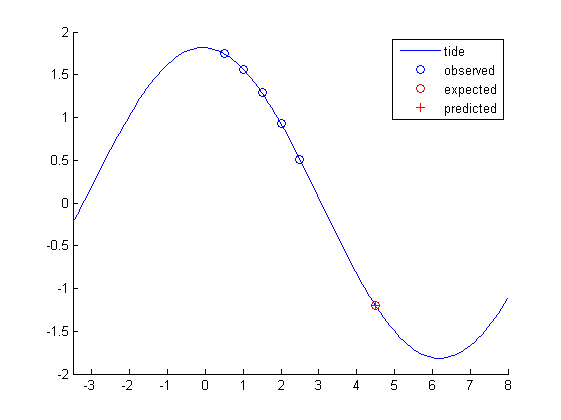
\includegraphics[width=0.6\textwidth]{simple_2h_1.png}
		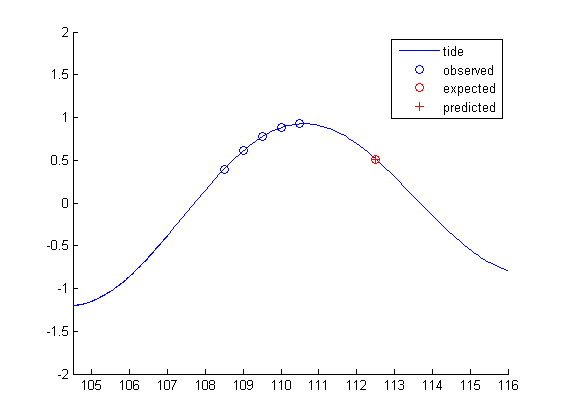
\includegraphics[width=0.6\textwidth]{simple_2h_2.png}
		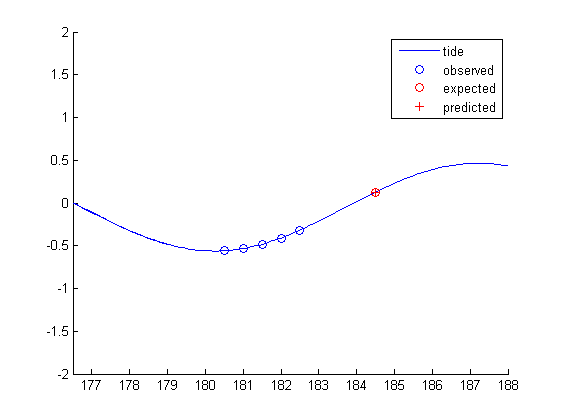
\includegraphics[width=0.6\textwidth]{simple_2h_3.png}
		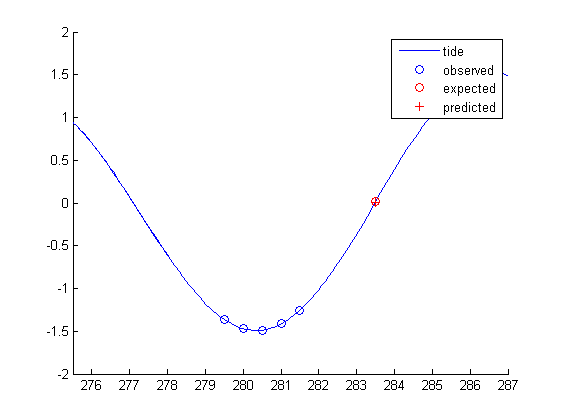
\includegraphics[width=0.6\textwidth]{simple_2h_4.png}
		\FloatBarrier
		
	\section{Predizione semplice massima}
		Per uno studio più approfondito dei limiti computazionali della rete lineare che simula il calcolo dell'altezza della marea si è provato quindi a determinare il numero massimo di ore di distanza dalla previsione, mantenendo lo scarto quadratico medio inferiore all'\textit{1\%}.\\
		\\
		Il risultato ottenuto, in via del tutto sperimentale, è di \textbf{36 ore} come intervallo massimo tra l'ultima marea osservata e la previsione che si vuole effettuare (osservando la marea ogni 2 ore) con un errore medio sull'altezza di marea inferiore all'\textbf{1\%}.
		Si noti che l'errore dell'\textit{1\%} risulta essere un valore molto basso, mentre \textit{36 ore} disponibili alla chiocciola per mettersi in salvo sul tronco di un albero sono più che sufficienti, per non dire eccessive: per errori più alti si può facilmente raggiungere un numero di ore per la previsione molto più alto, anche se inutile a fini pratici.\\
		\\
		Per riprodurre queste simulazioni basta impostare le variabili \textit{int} e \textit{forecast} a \textit{2} e \textit{36} rispettivamente (Codice \ref{lst:tideLin}).\\
		Di seguito alcuni grafici relativi a queste simulazioni:\\
		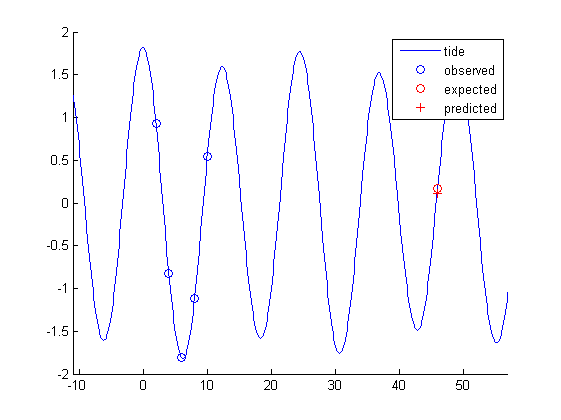
\includegraphics[width=0.6\textwidth]{simple_max_1.png}
		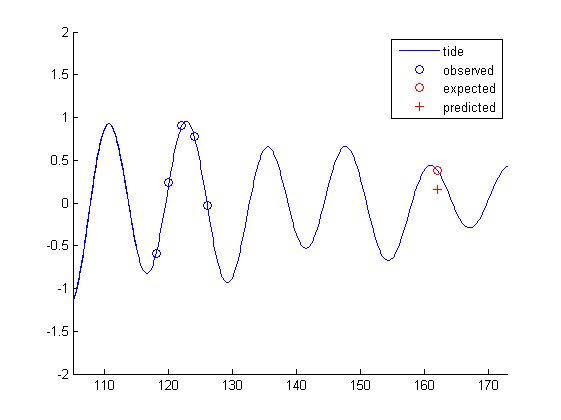
\includegraphics[width=0.6\textwidth]{simple_max_2.png}
		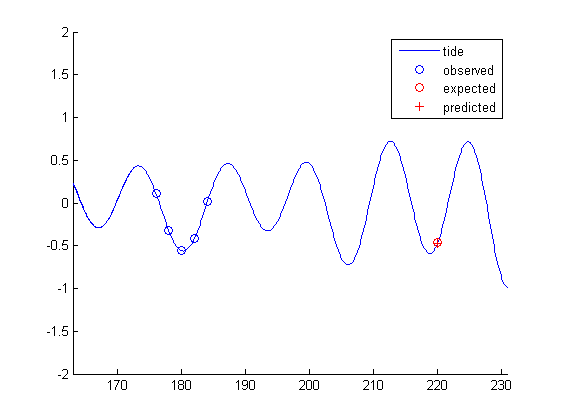
\includegraphics[width=0.6\textwidth]{simple_max_3.png}
		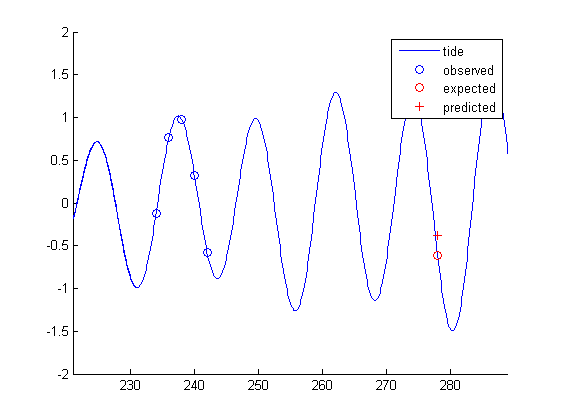
\includegraphics[width=0.6\textwidth]{simple_max_4.png}
		\FloatBarrier
	\chapter{Approssimazione di funzioni}
	\label{chapterApprossimazioniFunzioni}
	\minitoc \mtcskip
	\lettrine{Q}{}uesto capitolo tratta dell'approssimazione di funzioni tramite polinomi. Spesso infatti � necessario approssimare, all'interno di un calcolatore, la forma funzionale di una certa funzione $f:[a,b]\subset\mathbb{R}\rightarrow\mathbb{R}$ in quanto la sua forma funzionale potrebbe essere troppo complessa o addirittura non nota.\\
	In generale, assumeremo di essere a conoscenza di un insieme di $n+1$ ascisse distinte,
	\begin{equation}
		\label{ascisse}
		a\leq x_0<x_1<\dots<x_n\leq b,
	\end{equation}
	dette \textbf{ascisse di interpolazione}, e dei valori assunti dalla funzione in tali punti.
	\section{Interpolazione polinomiale}
		Siano note le coppie
		$$(x_i,f_i),\quad i=0,1,\dots,n,\quad f_i\equiv f(x_i),$$
		ricerchiamo un \textbf{polinomio interpolante} la funzione $f(x)$ sulle ascisse (\ref{ascisse}), detto $p(x)\in\Pi_n$, che assuma gli stessi valori di $f$ sulle ascisse di interpolazione (\ref{ascisse}), ovvero tale che
		\begin{equation}
			\label{condizioniInterp}
			p(x_i)=f_i,\qquad i=0,1,\dots,n.
		\end{equation}
		\begin{teo}
			Date le ascisse (\ref{ascisse}), esiste ed � unico il polinomio $p(x)\in\Pi_n$ interpolante $f$ sulle ascisse (\ref{ascisse}).
		\end{teo}
		Per determinare tale polinomio interpolante, essendo unico, si tratter� di determinare gli $n+1$ coefficienti dei monomi presenti nel polinomio, che equivale a risolvere il seguente sistema lineare:
		\begin{equation}
			\label{sistemaVandermonde}
			V\underline{a}=\underline{f},
		\end{equation}
		\[
			\begin{pmatrix}
				x_0^0 & x_0^1 & \dots & x_0^n\\
				x_1^0 & x_1^1 & \dots & x_1^n\\
				\vdots & \vdots &  & \vdots\\
				x_n^0 & x_n^1 & \dots & x_n^n\\
			\end{pmatrix}
			\begin{pmatrix}
				a_0\\
				a_1\\
				\vdots\\
				a_n
			\end{pmatrix}
			=
			\begin{pmatrix}
				f_0\\
				f_1\\
				\vdots\\
				f_n
			\end{pmatrix}.
		\]
		Infatti un generico polinomio avr� la forma
		\begin{equation}
			\label{genericoPolinomio}
			p(x)=\sum_{k=0}^{n}a_kx^k,
		\end{equation}
		e la matrice $V$, che � la trasposta della \textbf{matrice di Vandermonde}, risulta essere nonsingolare. Tuttavia, una delle propriet� note della matrice di Vandermonde, � che essa diviene rapidamente \textit{malcondizionata} al crescere di $n$, ovvero del numero di ascisse di interpolazione. Quindi esamineremo metodi alternativi per la determinazione del polinomio $p(x)$ interpolante $f(x)$.

	\section{Forma di Lagrange e forma di Newton}
		\label{sezFormaLagrangeNewton}
		Il problema (\ref{sistemaVandermonde}) deriva dall'aver scelto, come base per lo spazio vettoriale dei polinomi $\Pi_n$, la regolare \textbf{base delle potenze}, $\{x^0, x^1,\dots,x^n\}$. Per riformulare il problema, ottenendo propriet� pi� favorevoli, � necessario quindi cambiare base per $\Pi_n$.\\
		\\
		\textbf{\underline{Base di Lagrange}:}\\
		La \textit{base di Lagrange} � costituita da i seguenti polinomi:
		\begin{equation}
			\label{lagrange}
			L_{k,n}(x)=\mathlarger\prod_{
			\begin{subarray}{c}
				j=0\\
				j\neq k
			\end{subarray}
			}^{n}\frac{x-x_j}{x_k-x_j},\qquad k=0,1,\dots,n,
		\end{equation}
		dove $L_{k,n}(x)$ indica il $k$-esimo polinomio della base di Lagrange di grado $n$ calcolato in $x$. Osserviamo che, essendo le ascisse (\ref{ascisse}) tutte distinte tra loro, i polinomi (\ref{lagrange}) risultano essere ben definiti.
		\begin{lem}
			\label{lem4.1}
			Dati i polinomi di Lagrange (\ref{lagrange}) definiti sulle ascisse (\ref{ascisse}),
			\[
				L_{k,n}(x_i)=
				\begin{cases}
					1,&\quad\text{se }k=i,\\
					0,&\quad\text{se }k\neq i.
				\end{cases}
			\]
			Inoltre risulta che:
			\begin{itemize}
				\item essi hanno \textit{grado esatto $n$} ed il \textbf{coefficiente principale} (ovvero il coefficiente del termine di grado massimo) di $L_{k,n}(x)$ �
					\begin{equation}
						\label{coeffPrincipaleLagrange}
						c_{k,n}=\frac{1}{\prod_{
						\begin{subarray}{c}
							j=0\\
							j\neq k
						\end{subarray}}^{n}(x_k-x_j)}, \qquad k=0,1,\dots,n;
					\end{equation}
				\item essi sono \textit{linearmente indipendenti} tra loro, costituendo quindi una \textit{base} per $\Pi_n$.
			\end{itemize}
		\end{lem}

		\begin{teo}[Forma di Lagrange]
			Il polinomio
			\begin{equation}
				\label{formaLagrange}
				p(x)=\sum_{k=0}^{n}f_kL_{k,n}(x)
			\end{equation}
			appartiene a $\Pi_n$ e soddisfa i vincoli di interpolazione (\ref{condizioniInterp}), ovvero interpola $f(x)$ sulle ascisse (\ref{ascisse}).
		\end{teo}
		Quindi la forma di Lagrange (\ref{formaLagrange}) consente di ottenere in modo immediato il polinomio interpolante di grado richiesto (infatti i coefficienti del polinomio interpolante, rispetto alla base di Lagrange, risultano essere esattamente i valori $\{f_i\}$). Tuttavia questa apparente semplicit� formale non si presta a soddisfare un requisito, spesso richiesto in questo tipo di problema, che � quello di generare il polinomio interpolante in maniera \textit{incrementale}. In particolare vorremmo poter ottenere, dal polinomio $p_r(x)$, gi� calcolato sulle ascisse $x_0,x_1,\dots x_r$, il polinomio $p_{r+1}(x)$ di grado successivo, calcolato sulle ascisse precedenti pi� un'ulteriore ascissa $x_{r+1}$, in maniera relativamente semplice.\\
		Definiamo, allora, a questo scopo, un'ulteriore base di $\Pi_n$.\\
		\\
		\textbf{\underline{Base di Newton}:}\\
		La \textit{base di Newton} � definita da i seguenti polinomi:
		\begin{align}
			&w_0(x)\equiv 1,\notag\\
			\label{baseNewton}
			&w_{k+1}(x) = (x-x_k)w_k(x),\qquad k=0,1,2,\dots.
		\end{align}
		Si verifica facilmente che (vedi -->ref{es4.4}) la base di Newton gode delle seguenti propriet�:
		\begin{lem}
			\label{lem4.2}
			Con riferimento ai polinomi (\ref{baseNewton}) della base di Newton, per ogni $k=0,1,2,\dots$, si ha che:
			\begin{itemize}
				\item $w_k(x)\in\Pi_k'$, dove $\Pi_k'$ indica lo \textit{spazio vettoriale} dei \textbf{polinomi monici} di grado $k$ (un polinomio si dice \textbf{monico} se il suo \textit{coefficiente principale} � pari a $1$),
				\item $w_{k+1}(x)=\prod_{j=0}^{k}(x-x_j)$,
				\item $w_{k+1}(x_j)=0$, per $i\leq k$,
				\item $w_0(x),\dots,w_k(x)$ costituiscono una base per $\Pi_k$.
			\end{itemize}
		\end{lem}

		\begin{teo}[Forma di Newton]
			La famiglia dei polinomi di Newton interpolanti $\{p_r(x)\}_{r=0}^{n}$ tali che:
			$$p_r(x)\in\Pi_r,\qquad p_r(x_i)=f_i,\qquad i=0,\dots,r,$$
			� generata ricorsivamente come segue:
			\begin{align}
				&p_0(x)=f_0w_0(x),\notag\\
				\label{polinomiNewton}
				&p_r(x)=p_{r-1}(x)+f[x_0,x_1,\dots,x_r]w_r(x),\qquad r=1,\dots,n,
			\end{align}
			dove il fattore $f[x_0,x_1,\dots,x_r]$ � detto \textbf{differenza divisa} di ordine $r$ della funzione $f(x)$ sulle ascisse $x_0,x_1,\dots,x_r$, e vale
			\begin{equation}
				\label{differenzeDivise}
				f[x_0,x_1,\dots,x_r]=\sum_{k=0}^{r}\frac{f_k}{
				\prod_{
				\begin{subarray}{c}
					j=0\\
					j\neq k
				\end{subarray}}^{r}(x_k-x_j)}.
			\end{equation}
		\end{teo}
		\lstinputlisting[caption={Calcolo di una differenza divisa.}]{code/differenzaDivisa.m}
		Data la natura iterativa della generazione dei polinomi (\ref{polinomiNewton}) di Newton possiamo utilizzare la seguente forma della forma di Newton soddisfacente le (\ref{condizioniInterp}):
		\begin{equation}
			\label{polinomioNewtonCompatto}
			p(x)\equiv p_n(x)=\sum_{r=0}^{n}f[x_0,\dots,x_r]w_r(x),
		\end{equation}
		infatti $f[x_0]=f_0$.\\
		Possiamo quindi calcolare la forma di Newton del polinomio interpolante tramite il seguente Codice:
		\lstinputlisting[caption={Forma di Newton del polinomio interpolante.}]{code/formaNewton.m}
		Si osservi che il denominatore del $k$-esimo polinomio della base di Lagrange di grado $n$ (\ref{lagrange}) e del corrispondente coefficiente principale (\ref{coeffPrincipaleLagrange}) � dato da $w_{n+1}'(x)$, mentre il denominatore di ogni termine delle differenze divise (\ref{differenzeDivise}) � dato da $w_{r+1}'(x_k)$. Ad esempio, per $n$ (o $k$) uguale a $4$ abbiamo
		\begin{align*}
			&w_4(x)=(x-x_3)(x-x_2)(x-x_1)(x-x_0),\\
			&w_4'(x)
				\begin{aligned}[t]
					&=\partial[(x-x_3)(x-x_2)]\cdot(x-x_1)(x-x_0)+(x-x_3)(x-x_2)\cdot\partial[(x-x_1)(x-x_2)]=\\
					&=(2x-x_3-x_2)(x-x_1)(x-x_0)+(x-x_3)(x-x_2)(2x-x_1-x_0),
				\end{aligned}
		\end{align*}
		e per, ad esempio, $k=1$ otteniamo
		\begin{align*}
			w_4'(x_1)&=(2x_1-x_3-x_2)(x_1-x_1)(x_1-x_0)+(x_1-x_3)(x_1-x_2)(2x_1-x_1-x_0)=\\
			&=(x_1-x_3)(x_1-x_2)(x_1-x_0).
		\end{align*}
		Quindi risulta che le differenze divise (\ref{differenzeDivise}) costituiscono i coefficienti del polinomio interpolante (\ref{condizioniInterp}) rispetto alla base di Newton (ma non, ad esempio, rispetto alla base delle potenze!).
		\begin{teo}
			\label{teoPropriet�DiffDiv}
			Le differenze divise (\ref{differenzeDivise}) godono delle seguenti propriet�:
			\begin{enumerate}
				\item siano $\alpha,\beta\in\mathbb{R}$ e $f(x),g(x)$ due funzioni in una variabile reale, allora
					$$(\alpha\cdot f+\beta\cdot g)[x_0,\dots,x_r]=\alpha\cdot f[x_0,\dots,x_r]+\beta\cdot g[x_0,\dots,x_r];$$
				\item per ogni $\{i_0,\dots,i_r\}$ permutazione di $\{0,\dots,r\}$,
					$$f[x_{i_0},\dots,x_{i_r}]=f[x_0,\dots,x_r],$$
					ovvero non conta l'ordine con cui compaiono le ascisse nella differenza divisa;
				\item sia $f(x)=\sum_{i=0}^{k}a_ix^i\in\Pi_k$, allora,
					\begin{equation}
						\label{diffDiviseTaylor}
						f[x_0,\dots,x_r]=
						\begin{cases}
							a_k, &\quad\text{se }r=b,\\
							0, &\quad\text{se }r>b;
						\end{cases}
					\end{equation}
				\item pi� in generale, se $f(x)\in C^{(r)}$, allora
					\begin{equation}
						\label{diffDivXi}
						f[x_0,\dots,x_r]=\frac{f^{(r)}(\xi)}{r!},\qquad\xi\in[\min_{i}x_i,\max_{i}x_i];
					\end{equation}
				\item
					\begin{equation}
						\label{diffDivOrdineInferiore}
						f[x_0,x_1,\dots,x_{r-1},x_r]=\frac{f[x_1,\dots,x_r]-[x_0,\dots,x_{r-1}]}{x_r-x_0}.
					\end{equation}
			\end{enumerate}
		\end{teo}

		Si pu� osservare che, per la (\ref{diffDiviseTaylor}), se $x_0=\dots=x_n$, il polinomio (\ref{polinomioNewtonCompatto}) coincide con il polinomio di Taylor di $f(x)$ di punto iniziale $x_0$.\\
		Grazie alla propriet� (\ref{diffDivOrdineInferiore}), possiamo costruire una differenza divisa di ordine $r$ se conosciamo due differenze divise di ordine $r-1$ che differiscano di una sola ascissa. Ricordando allora che
		$$f[x_i]=f_i,\qquad i=0,1,\dots,n,$$
		possiamo costruire, in modo iterativo, la seguente tabella triangolare inferiore:
		\begin{center}
			\begin{tabular}{c|c c c c c}
				& $0$ & $1$ & \dots & $n-1$ & $n$\\
				\hline
				$x_0$ & \fbox{$f[x_0]$} & & & &\\
				$x_1$ & $f[x_1]$ & \fbox{$f[x_0,x_1]$} & & &\\
				$x_2$ & $f[x_2]$ & $f[x_1,x_2]$ & $\ddots$ & &\\
				$\vdots$ & $\vdots$ & $\vdots$ & & &\\
				$x_{n-1}$ & $f[x_{n-1}]$ & $f[x_{n-2},x_{n-1}]$ & \dots & \fbox{$f[x_0,\dots,x_{n-1}]$} &\\
				$x_n$ & $f[x_n]$ & $f[x_{n-1},x_n]$ & \dots & $f[x_1,\dots,x_n]$ & \fbox{$f[x_0,x_1,\dots,x_n]$}
			\end{tabular}
		\end{center}
		La diagonale principale (elementi messi in evidenza) contiene i coefficienti del polinomio interpolante nella forma di Newton (\ref{polinomioNewtonCompatto}). Le colonne di tale tabella devono essere calcolate da sinistra verso destra: la prima coincide con i valori assunti dalla funzione nelle ascisse di interpolazione ed �, quindi, data; ogni elemento delle colonne successive alla prima viene calcolato applicando la (\ref{diffDivOrdineInferiore}) con l'elemento nella colonna immediatamente precedente (sulla stessa riga) e l'elemento nella colonna e nella riga immediatamente precedenti. Inoltre si nota che gli elementi di una determinata colonna non sono pi� utilizzati una volta calcolati gli elementi della colonna successiva (sulla stessa riga), e quindi per il calcolo delle differenze divise pu� essere utilizzato un unico vettore che viene riscritto di volta in volta fino ad ottenere l'ultima differenza divisa.\\
		Con questi accorgimenti, possiamo definire la seguente implementazione in \textsc{Matlab} per il calcolo delle differenze divise:
		\lstinputlisting[caption={Calcolo delle differenze divise.}, label=lst:differenzeDivise]{code/differenzeDivise.m}

		\subsection{Interpolazione di Hermite}
			Supponiamo adesso di avere le ascisse di interpolazione numerate nel modo seguente:
			$$a\leq x_0<x_{\frac{1}{2}}<x_1<x_{1+\frac{1}{2}<\dots x_n<x_{n+\frac{1}{2}\leq b}},$$
			in modo tale che le condizioni di interpolazione per il polinomio interpolante $p(x)\in\Pi_{2n+1}$ diventano:
			$$p(x_i)=f_i,\qquad p(x_{i+\frac{1}{2}}=f_{i+\frac{1}{2}},\qquad i=0,1,\dots,n).$$
			Facciamo allora tendere le ascisse di indice con indice frazionario verso quelle immediatamente precedenti di indice intero:
			$$x_{i+\frac{1}{2}}\rightarrow x_i,\qquad i=0,1,\dots,n.$$
			Quindi, assumendo (fino alla fine della sezione) che $f(x)\in C^{(1)}$, otteniamo che
			\begin{align*}
				\frac{f(x_{i+\frac{1}{2}})-f(x_i)}{x_{i+\frac{1}{2}-x_i}}&=f[x_i,x_{i+\frac{1}{2}}] \footnoteOP{\rightarrow} f[x_i,x_i] =\\
				&=\frac{f'(\xi)}{1!} \footnoteOP{\equiv} f'(x_i),\quad i=0,1,\dots,n.
			\end{align*}
			%-------- FOOTNOTES --------
			\addtocounter{footnote}{-1}
			\footnotetext{Per la (\ref{diffDivOrdineInferiore}).}
			\stepcounter{footnote}
			\footnotetext{Con $\xi\in[\max\{x_i\},\min\{x_i\}]$, per la (\ref{diffDivXi}).}
			%-------- end FOOTNOTES --------
			
			Quindi abbiamo che le ascisse di interpolazione divengono
			\begin{equation}
				\label{ascisseHermite}
				a\leq x_0=x_0<x_1=x_1<\dots<x_n=x_n\leq b,
			\end{equation}
			cos� che il polinomio interpolante (\ref{polinomioNewtonCompatto}) risulta ancora ben definito e si vede che soddisfa i seguenti vincoli di interpolazione:
			\begin{itemize}
				\item $p(x_i)=f(x_i),$
				\item $p'(x_i)=f'(x_i),\quad i=0,1,\dots,n$.
			\end{itemize}
			Questo polinomio allora, detto \textbf{polinomio interpolante di Hermite}, risulta interpolare sia la funzione che la sua derivata nelle ascisse di interpolazione distinte in (\ref{ascisseHermite}).\\
			Notare che, per $n=0$, il polinomio di Hermite coincide con il polinomio di Taylor di primo grado e punto iniziale $x_0$:
			$$p(x)=f[x_0]+f[x_0,x_0](x-x_0)=f(x_0)+f'(x_0)(x-x_0).$$
			In generale, per un generico $n$, il polinomio di Hermite avr� una forma del tipo:
			\begin{align*}
				p(x) &= f[x_0]+\\
				&+ f[x_0,x_0](x-x_0)+\\
				&+f[x_0,x_0,x_1](x-x_0)^2+\\
				&+f[x_0,x_0,x_1,x_1](x-x_0)^2(x-x_1)+\\
				&+f[x_0,x_0,x_1,x_1,x_2](x-x_0)^2(x-x_1)^2+\\
				&\vdots\\
				&+f[x_0,x_0,x_1,x_1,\dots,x_n,x_n](x-x_0)^2\dots(x-x_{n-1})^2(x-x_n).
			\end{align*}
			I coefficienti del polinomio di Hermite vengono calcolati tramite una versione ottimizzata del Codice \ref{lst:differenzeDivise}. Il Codice \ref{lst:differenzeDiviseHermite} prende in input il vettore
			$$f(x_0), f'(x_0), f(x_1), f'(x_1),\dots,f(x_n),f'(x_n),$$
			che viene riscritto con le differenze divise. Si osservi che le derivate della funzione sulle ascisse di interpolazione non devono essere riscritte al primo ciclo, essendo $f[x_i,x_i]=f'(x_i)$, per $i=0,1,\dots,n$.
			\lstinputlisting[caption={Calcolo delle differenze divise per il polinomio di Hermite.}, label=lst:differenzeDiviseHermite]{code/differenzeDiviseHermite.m}
			\lstinputlisting[caption={Calcolo del polinomio interpolante di Hermite.}]{code/hermite.m}
			
	\section{Errore nell'interpolazione}
		\label{sezErrInterp}
		Studiamo adesso di quanto si sbaglia utilizzando il polinomio interpolante al posto della funzione originale.
		\begin{defi}
			Sia $p(x)\in\Pi_n$ il polinomio interpolante soddisfacente le condizioni d'interpolazione (\ref{condizioniInterp}). Si dice \textbf{errore di interpolazione} la quantit�
			\begin{equation}
				\label{erroreInterpolazione}
				e(x)=f(x)-p(x),
			\end{equation}
			ovvero l'errore commesso nell'approssimare $f(x)$ mediante il suo polinomio interpolante $p(x)$.
		\end{defi}
		Ovviamente, per le condizioni (\ref{condizioniInterp}), risulta che
		$$e(x_i)=0,\qquad i=0,1,\dots,n,$$
		ovvero l'errore � nullo sulle ascisse di interpolazione.
		\begin{teo}
			Sia $p(x)$ il polinomio il polinomio (\ref{polinomioNewtonCompatto}) soddisfacente le (\ref{condizioniInterp}). Il corrispondente \textit{errore di interpolazione} (\ref{erroreInterpolazione}) vale
			\begin{equation}
				\label{espressioneErroreInterpolazione}
				e(x)=f[x_0,x_1,\dots,x_n,x]w_{n+1}(x),
			\end{equation}
			ovvero il termine ``mancante'' in $p(x)$ se si fosse interpolato su un'ulteriore ascissa corrispondente ad $x$.
		\end{teo}
		\begin{cor}
			Se $f(x)\in C^{(n+1)}$, allora
			$$e(x)=\frac{f^{(n+1)}(\xi_x)}{(n+1)!}w_{n+1}(x),\qquad\xi_x\in[\min\{x_0,x\},\max\{x_n,x\}].$$
			L'ascissa minima risulta essere $x_0$ o $x$, in quanto le ascisse (\ref{ascisse}) sono ordinate in senso crescente. Analogamente per la massima.
		\end{cor}
		Quindi la struttura dell'errore d'interpolazione ci dice che esso � composto sostanzialmente da due parti:
		\begin{itemize}
			\item l'una, $\frac{f^{(n+1)}(\xi_x)}{(n+1)!}$, dipende dalle propriet� di regolarit� della funzione $f(x)$,
			\item l'altra, $w_{n+1}(x)$, che dipende esclusivamente dalla scelta delle ascisse di interpolazione.
		\end{itemize}
		Risulta che $w_{n+1}(x)$ oscilla per $x\in[x_0,x_n]$, annullandosi nelle ascisse di interpolazione (\ref{ascisse}). Al contrario, $|w_{n+1}(x)|$ cresce con la stessa velocit� di $x^{n+1}$ al di fuori dell'intervallo di interpolazione, ovvero per $x<x_0$ o $x>x_n$. Se ne conclude che il polinomio $p(x)$ pu� essere convenientemente utilizzato per approssimare $f(x)$ soltanto all'interno dell'intervallo $[x_0,x_n]$. Per questo si parla di \textbf{interpolazione} polinomiale anzich� di \textit{estrapolazione} (che invece si occupa dell'utilizzo di $p(x)$ al di fuori di tale intervallo). Inoltre si osserva che, aumentando opportunamente il numero delle ascisse di interpolazione, l'errore di interpolazione commesso nell'intervallo $[a,b]$ decresce.

	\section{Condizionamento del problema}
		Come tutti i problemi fin'ora affrontati, dedichiamoci adesso allo studio del \textit{condizionamento del problema} della valutazione del polinomio interpolante. Consideriamo quindi, come unici dati di ingresso, i valori $\{f_i\}$ assunti dalla funzione $f(x)$ sulle ascisse di interpolazione (\ref{ascisse}). L'analisi del condizionamento verr� condotta sugli errori assoluti.\\
		Abbiamo quindi che il polinomio interpolante \textit{esatto}, in forma di Lagrange, � dato da
		$$p(x)=\sum_{k=0}^{n}f_kL_{k,n}(x),$$
		mentre il polinomio interpolante costruito a partire dai \textit{dati perturbati} �
		$$\tilde{p}(x)=\sum_{k=0}^{n}\tilde{f}_kL_{k,n}(x),$$
		dove $\tilde{f}_i\equiv\tilde{f}(x_i)$, essendo $\tilde{f}(x)$ una perturbazione di $f(x)$.
		Si ottiene quindi
		\begin{align*}
			|p(x)-\tilde{p}(x)| &= |\sum_{k=0}^{n}f_kL_{k,n}(x) - \sum_{k=0}^{n}\tilde{f}_kL_{k,n}(x)|= |\sum_{k=0}^{n}(f_k-\tilde{f}_k)L_{k,n}(x)|=\\
			&= |\sum_{k=0}^{n}(f_k-\tilde{f}_k)\cdot L_{k,n}(x)|\leq \sum_{k=0}^{n}|(f_k-\tilde{f}_k)|\cdot|L_{k,n}(x)|\leq\footnotemark\\
			&\leq \left(\sum_{k=0}^{n}|L_{k,n}(x)|\right)\max_{k}|f_k-\tilde{f}_k| \footnoteOP{\equiv} \lambda_n(x)\max_{k}|f_k-\tilde{f}_k|,
		\end{align*}
		%-------- FOOTNOTES --------
		\addtocounter{footnote}{-1}
		\footnotetext{Per la \textit{disuguaglianza triangolare}, il valore assoluto della somma � minore o uguale alla somma dei valori assoluti.}
		\stepcounter{footnote}
		\footnotetext{Viene maggiorata la differenza tra i vari $f_k$ ed $\tilde{f}_k$ e raccolta come fattore comune per tutti i polinomi $|L_{k,n}(x)|$.}
		%-------- end FOOTNOTES --------
		
		dove la funzione $\lambda_n(x)\equiv\left(\sum_{k=0}^{n}|L_{k,n}(x)|\right)$ � detta \textbf{funzione di Lebesgue}, che si vede dipende soltanto dalla scelta delle ascisse di interpolazione (in quanto i polinomi $|L_{k,n}(x)|$ che la compongono dipendono soltanto dalle ascisse (\ref{ascisse})). Considerando, come avevamo gi� concluso nella Sezione \ref{sezErrInterp}, il caso in cui $x\in[a,b]$ (vedi (\ref{ascisse})), definiamo la norma in $C^{(0)}$ come
		\begin{equation}
			\label{normaC0}
			||f||=\max_{a\leq x\leq b}|f(x)|.
		\end{equation}
		Volendo quindi stimare una maggiorazione per la quantit� $|p(x)-\tilde{p}(x)|$, avremo che
		\begin{equation}
			\label{costanteLebesgue}
			||p-\tilde{p}||\leq ||\lambda_n||\cdot||f-\tilde{f}||\equiv\Lambda_n||f-\tilde{f}||,
		\end{equation}
		dove la quantit� $\Lambda_n$ � detta \textbf{costante di Lebesgue}, la quale dipende esclusivamente dalla scelta delle ascisse di interpolazione e dall'intervallo $[a,b]$ considerato.\\
		Osserviamo che, essendo nella (\ref{costanteLebesgue}) la quantit� $||f-\tilde{f}||$ una maggiorazione dell'errore assoluto presente sui dati in ingresso e, analogamente, la quantit� $||p-\tilde{p}||$ una maggiorazione dell'errore assoluto commesso sul risultato, si ha che la \textit{costante di Lebesgue}, $\Lambda_n$, rappresenta il \textbf{numero di condizionamento} del problema di valutazione del polinomio interpolante. A questo proposito � noto che:
		\begin{itemize}
			\item $\Lambda_n\geq O(\log n)\rightarrow\infty$ per $\rightarrow\infty$. Pertanto il problema diviene progressivamente \textit{malcondizionato} al crescere del numero di ascisse di interpolazione $n$, ed inoltre $\Lambda_n$ crescer� almeno con velocit� \textit{logaritmica};
			\item la scelta di ascisse di interpolazione equidistanti
			\begin{equation}
				\label{ascisseEquidistanti}
				x_i=a+i\cdot h,\qquad i=0,1,\dots,n,\qquad h=\frac{b-a}{n},
			\end{equation}
			per quanto possa sembrare logica, genera una successione $\{\Lambda_n\}$ che \textit{diverge} con velocit� approssimativamente \textit{esponenziale}, per $n\rightarrow\infty$. Non rappresenta quindi la scelta ottimale, specialmente per valori elevati di $n$.
		\end{itemize}
		\lstinputlisting[caption={Calcolo delle ascisse di interpolazione equidistanti.}]{code/ascisseEquidistanti.m}
		Studiamo adesso che relazione intercorre tra l'errore dell'interpolazione ed il condizionamento del problema.
		\begin{defi}
			Data una funzione $f(x)$ continua in $[a,b]$, il polinomio $p^*(x)\in\Pi_n$ tale che
			\begin{equation}
				\label{poliMigliorAppr}
				||f-p^*||=\min_{p\in\Pi_n}||f-p||,
			\end{equation}
			si dice \textbf{polinomio di miglior approssimazione} di grado $n$ di $f(x)$ sull'intervallo $[a,b]$.
		\end{defi}
		\begin{teo}
			Assegnata una funzione $f(x)$ continua in $[a,b]$, esiste il polinomio $p^*(x)\in\Pi_n$ di miglior approssimazione (vedi (\ref{poliMigliorAppr})) di $f(x)$ su $[a,b]$.
		\end{teo}
		\begin{teo}
			Sia $p^*(x)$ il polinomio di miglior approssimazione di grado $n$ di $f(x)$. Allora per l'errore di interpolazione (\ref{erroreInterpolazione}) vale
			\begin{equation}
				\label{errore+migliorAppr}
				||e||\leq (1+\Lambda_n)||f-p^*||.
			\end{equation}
		\end{teo}
		Quindi non � detto che, al crescere di $n$, l'errore decresca, in quanto la costante di Lebesgue diverge esponenzialmente.\\
		Introduciamo il concetto di \textbf{modulo di continuit�} di una funzione:
		$$\omega(f;h)\equiv\sup\{|f(x)-f(y)|:x,y\in[a,b],|x-y|\leq h\},$$
		dove $h>0$ � un parametro assegnato. Si osserva che:
		\begin{itemize}
			\item se $f\in C^{0}$, allora $\omega(f;h)\rightarrow 0$, per $h\rightarrow 0$: infatti diminuendo sempre di pi� l'intervallo $h$, ed essendo la funzione continua, i valori della $f$ si avvicinano sempre di pi�;
			\item se $f(x)$ � \textit{Lipschitziana} con costante $L$, allora $\omega(f;h)\leq Lh$. Ad esempio, se $f(x)\in C^{(1)}$, $L=\max_{a\leq x\leq b}|f'(x)|\equiv||f'||$.
		\end{itemize}
		\begin{teo}[Jackson]
			Per il polinomio di miglio approssimazione (\ref{poliMigliorAppr}) di una funzione $f(x)\in C^{(0)}$ si ha:
			\begin{equation}
				\label{erroreMigliorAppr}
				||f-p^*||\leq \alpha\cdot\omega\left(f;\frac{b-a}{n}\right),
			\end{equation}
			in cui la costante $\alpha$ � indipendente da $n$.
		\end{teo}
		Segue infine, per la (\ref{errore+migliorAppr}) e la (\ref{erroreMigliorAppr}), che, per una generica $f(x)$:
		$$||e||\leq \alpha(1+\Lambda_n)\omega\left(f;\frac{b-a}{n}\right).$$
		Quindi, concludendo e riassumendo questa Sezione e la precedente, � opportuno effettuare una scelta delle ascisse di interpolazione in modo tale che:
		\begin{enumerate}
			\item la costante di Lebesgue $\Lambda_n$ abbia una crescita moderata, preferibilmente logaritmica (che abbiamo visto essere quella ottimale), rispetto al grado $n$ del polinomio interpolante;
			\item sia minimizzata la quantit� $||w_{n+1}||$, come avevamo gi� dedotto in conclusione della Sezione \ref{sezErrInterp}.
		\end{enumerate}

	\section{Ascisse di Chebyshev}
		Quindi risulta chiaro che si tratta di scegliere le ascisse in modo da minimizzare la norma $||w_{n+1}||$. Ma la norma, per definizione, � il massimo di una funzione su un certo intervallo (vedi (\ref{normaC0})), ovvero si tratta di minimizzare un valore massimo: si deve allora cercare la soluzione del seguente \textbf{problema del minimassimo} (o \textbf{minmax}):
		$$\min_{a\leq x_0<\dots<x_n\leq b}||w_{n+1}||\equiv\min_{a\leq x_0<\dots<x_n\leq b}\;\max_{a\leq x \leq b}|w_{n+1}(x)|.$$
		Senza perdere di generalit� (vedi Esercizio \ref{es4.12}) assumiamo che
		$$[a,b]\equiv[-1,1].$$

		Definiamo allora la famiglia dei \textbf{polinomi di Chebyshev di prima specie}:
		\begin{align}
			&T_0(x)\equiv 1,\notag\\
			\label{chebyshevISpecie}
			&T_1(x)\equiv x,\\
			&T_{k+1}(x)\equiv 2xT_k(x)-T_{k-1}(x),\qquad k=1,2,\dots.\notag
		\end{align}
		Si possono dimostrare (per induzione) le seguenti propriet� dei polinomi di Chebyshev:
		\begin{enumerate}
			\item $T_k(x)$ � un polinomio di grado esatto $k$;
			\item il coefficiente principale di $T_k(x)$ � $2^{k-1}$, per $k=1,2,\dots$;
			\item la famiglia dei polinomi $\{\hat{T}_k\}$, dove
				$$\hat{T}_0(x)=T_0(x),\quad \hat{T}_k(x)=2^{1-k}T_k(x)=\frac{T_k(x)}{2^{k-1}},\quad k=1,2,\dots,$$
				� una famiglia di \textit{polinomi monici} (dal coefficiente principale uguale a $1$) di grado $k$, per $k=0,1,\dots$;
			\item possiamo parametrizzare i punti dell'intervallo $[-1,1]$ rispetto a $\theta$, ponendo
				$$x=\cos\theta,\qquad \theta\in[0,\pi].$$
				Inoltre, considerando che
				$$\cos(k\theta + \theta)+\cos(k\theta-\theta)=2\cos(k\theta)\cos(\theta)$$
				si ottiene
				$$T_k(x)\equiv T_k(\cos\theta)=\cos(k\theta),\qquad k=0,1,\dots.$$
		\end{enumerate}
		Sfruttando queste propriet� si ottiene:
		\begin{teo}
			\label{propriet�PolinomiChebyshev}
			Gli zeri di $T_k(x)$, tra loro distinti, sono dati da
			$$x_i^{(k)}=\cos\left(\frac{(2i+1)\pi}{2k}\right),\qquad i=0,1,\dots,k-1.$$
			Si pu� vedere che , per $x\in[-1,1]$, i valori estremi del polinomio $T_k(x)$ sono assunti nei punti
			$$\xi_i^{(k)}=\cos\left(\frac{i}{k}\pi\right),\qquad i=0,1,\dots,k,$$
			nei quali il polinomio assume i valori
			$$T_k(\xi_i^{(k)})=(-1)^i,\qquad i=0,1,\dots,k,$$
			quindi risulta che $||T_k||=1$ (cio� il valore massimo del polinomio � $1$, essendo un coseno).
			Inoltre, per $k=1,2,\dots,$
			\begin{equation}
				\label{minimaNormaPolMonici}
				||\hat{T}_k||=2^{1-k}=\min_{\varphi\in\Pi'_k}||\varphi||,
			\end{equation}
			ovvero il polinomio monico $\hat{T}_k$ ha norma minima tra tutti i polinomi monici di grado $k$.
		\end{teo}

		Si ottiene allora che, scegliendo come ascisse di interpolazione sull'intervallo $[-1,1]$ come
		\begin{equation}
			\label{ascisseChebyshev}
			x_{n-i}=\cos\left(\frac{2i+1}{2(n+1)}\pi\right),\qquad i=0,1,\dots,n,
		\end{equation}
		(dove l'indice $n-i$ serve a generare le ascisse in modo che siano ordinate in senso crescente rispetto al loro indice) si ha
		$$w_{n+1}(x)=\prod_{i=0}^{n}(x-x_i)\equiv\hat{T}_{n+1}(x),$$
		che rappresenta quindi la soluzione al problema del minimassimo, per la (\ref{minimaNormaPolMonici}).\\
		Per convertire queste ascisse nelle ascisse di interpolazione sull'intervallo $[a,b]$ basta effettuare la trasformazione (vedi Esercizio \ref{es4.12}):
		\begin{equation}
			\label{ascisseChebyshevAB}
			x_i|_{[a,b]}=\frac{a+b}{2}+\frac{b-a}{2}x_i|_{[-1,1]},\qquad i=0\dots,n.
		\end{equation}
		Il seguente Codice \textsc{Matlab} calcola le ascisse di Chebyshev secondo quanto appena visto:
		\lstinputlisting[caption={Calcolo delle ascisse di Chebyshev.}]{code/ascisseChebyshev.m}
		Scegliendo le ascisse \ref{ascisseChebyshevAB} di interpolazione, dette \textbf{ascisse di Chebishev}, si ottiene (per funzioni sufficientemente regolari)
		\begin{align*}
			||e||&\leq\frac{||f^{(n+1)}||}{(n+1)!}||w_{n+1}||=\\
			&= \frac{||f^{(n+1)}||}{(n+1)!}||\hat{T}_{n+1}||=\\
			&= \frac{||f^{(n+1)}||}{(n+1)!}2^{1-n-1}=\\
			&=\frac{||f^{(n+1)}||}{(n+1)!2^n},
		\end{align*}
		e la corrispondente costante di Lebesgue si vede valere
		$$\Lambda_n\approx\frac{2}{\pi}\log n,$$
		che risulta quindi avere una \textit{crescita ottimale}, per $n\rightarrow\infty$.\\
		\\
		Riassumendo, abbiamo concluso che scegliendo come ascisse di interpolazione le \textit{ascisse di Chebyshev} (\ref{ascisseChebyshev}) si ottengono i polinomi monici $\hat{T}_k$, $k=0,1,\dots,n$, che formano una \textit{base di Newton} sulla quale poter costruire il polinomio interpolante (come visto in Sezione \ref{sezFormaLagrangeNewton}), e tale che la norma del polinomio della base di grado $n+1$ (il primo polinomio ``mancante'' dalla base) sia minima (pari a $2^{-n}$).\\
		Si osserva che utilizzando le \textit{ascisse di Chebyshev} (\ref{ascisseChebyshev}) si perde la caratteristica della forma di Newton di poter generare polinomi interpolanti in modo incrementale in quanto le ascisse in questione dipendono dal grado $n$ del polinomio interpolante (compare la $n$ al denominatore) e quindi volendo determinare il polinomio interpolante di grado $n+1$ saremmo costretti a ricalcolare tutte le ascisse.

	\section{Interpolazione mediante funzioni \textit{spline}}
		Abbiamo visto che, al crescere del grado $n$ del polinomio interpolante, � necessario effettuare una scelta delle ascisse che non faccia crescere troppo velocemente la costante di Lebesgue $\Lambda_n$, che comunque crescer� almeno con velocit� logaritmica rispetto ad $n$. Tuttavia se $n$ rimane basso, il \textit{modulo di continuit�}
		$$w\left(f;\frac{b-a}{n}\right)$$
		non pu� tendere a $0$, con l'intervallo $[a,b]$ fissato.\\
		Allora:
		\begin{enumerate}
			\item consideriamo una partizione dell'intervallo originario,
				\begin{equation}
					\label{partizione}
					\Delta=\{a=x_0<x_1<\dots<x_n=b\},
				\end{equation}
				con
				\begin{equation}
					\label{hSpline}
					h=\max_{i=1,\dots,n}(x_i-x_{i-1})\rightarrow 0,\qquad n\rightarrow\infty;
				\end{equation}
			\item su ciascun sottointervallo $[x_{i-1},x_i]$ della partizione $\Delta$ consideriamo un polinomio di grado $m$ fissato interpolante la funzione $f(x)$ nei suoi estremi.
		\end{enumerate}
		In questo modo il problema del condizionamento passa in secondo piano in quanto il grado $m$ dei polinomi interpolanti rimane fissato mentre, al contempo (se $f\in C^{(0)}$),
		$$w(f;h)\rightarrow 0,\qquad n\rightarrow\infty.$$
		Questo nuovo tipo di funzione interpolante si dice \textbf{funzione polinomiale a tratti}, in quanto � rappresentabile da un polinomio in ogni sottointervallo, ma non nel suo insieme. Pi� in particolare:
		\begin{defi}
			La funzione $s_m(x)$ si dice \textbf{spline di grado $m$} sulla partizione $\Delta$ se
			\begin{enumerate}
				\item $s_m(x)\in C^{(m-1)}$ sull'intervallo $[a,b]$ e
				\item $s_m|_{[x_{i-1},x_i]}(x)\in\Pi_m$, per $i=1,\dots,n$.
			\end{enumerate}
		\end{defi}
		Se risulta che
		\begin{equation}
			\label{condizioniInterpSpline}
			s_m(x_i)=f_i,\qquad i=0,1,\dots,n,
		\end{equation}
		allora si dice che la \textit{spline} \textbf{interpola} la funzione $f(x)$ nei nodi della partizione $\Delta$.
		\begin{teo}
			\label{teoGradoSplineS'}
			Se $s_m(x)$ � una spline di grado $m$ sulla partizione (\ref{partizione}), allora $s'_m(x)$ � una spline di grado $m-1$ sulla stessa partizione.
		\end{teo}
		\begin{teo}
			L'insieme delle funzioni spline di grado $m$ definite sulla partizione (\ref{partizione}) � uno spazio vettoriale di dimensione $m+n$.
		\end{teo}
		Quest'ultimo teorema ci dice che sono necessarie $m+n$ condizioni indipendenti per poter individuare \textit{univocamente} la spline interpolante la funzione $f(x)$ sulla partizione $\Delta$ assegnata. Essendo allora le \textit{condizioni di interpolazione} (\ref{condizioniInterpSpline}) soltanto $n+1$, utilizzandolo soltanto queste condizioni possiamo individuare univocamente una spline di grado $1$, o \textbf{spline lineare}, che coincide con la spezzata congiungente i punti $\{(x_i,f_i)\}_{i=0,\dots,n}$:
		\begin{equation}
			\label{splineLineare}
			s_1|_{[x_{i-1},x_i]}(x)=\frac{(x-x_{i-1})f_i+(x_i-x)f_{i-1}}{x_i-x_{i-1}}.
		\end{equation}
		Risulta quindi necessario, per spline interpolanti di ordine superiore al primo, introdurre ulteriori condizioni (in particolare, $m-1$ condizioni aggiuntive rispetto alle condizioni di interpolazione (\ref{condizioniInterpSpline})) per definire la spline interpolante in maniera univoca.
	\section{\textit{Spline} cubiche}
		Le \textbf{spline cubiche} sono spline interpolanti di grado $3$. � quindi necessario imporre $2$ condizioni aggiuntive, oltre alle (\ref{condizioniInterpSpline}), per poter definire univocamente tale spline interpolante. In particolare, a seconda di quali condizioni sceglieremo di imporre, si avranno diversi tipi di \textit{spline cubica}.\\
		\\
		\textbf{\underline{\textit{Spline} naturale}:}\\
		La \textit{spline} naturale consiste nel fissare le seguenti condizioni aggiuntive:
		$$s''_3(a)=0,\qquad s''_3(b)=0,$$
		ovvero viene imposto che la derivata seconda della spline negli estremi della partizione $\Delta$ si annulli.\\
		\\
		\textbf{\underline{\textit{Spline} completa}:}\\
		Supponendo di conoscere i valori della derivata prima $f'(x)$ della funzione negli estremi della partizione, nel caso della \textit{spline} completa si impongono le seguenti condizioni.
		$$s'_3(a)=f'(a),\qquad s'_3(b)=f'(b).$$
		\\
		\textbf{\underline{\textit{Spline} periodica}:}\\
		Se la funzione da interpolare � periodica e l'intervallo $[a,b]$ contiene un numero intero di periodi della funzione, allora conviene utilizzare la \textit{spline} peridica, che consiste nell'imporre le condizioni
		$$s'_3(a)=s'_3(b),\qquad s''_3(a)=s''_3(b).$$
		\\
		\textbf{\underline{Condizioni \textit{not-a-knot}}:}\\
		In questo caso, per far s� che le condizioni di interpolazione (\ref{condizioniInterpSpline}) siano sufficienti a determinare la \textit{spline} cubica, si impone che lo stesso polinomio di terzo grado costituisca la restrizione della \textit{spline} sull'intervallo $[x_0,x_1]\cup[x_1,x_2]$ e, allo stesso modo, lo stesso polinomio di $\Pi_3$ costituisca la restrizione della \textit{spline} sull'intervallo $[x_{n-2},x_{n-1}]\cup[x_{n-1},x_n]$. In poche parole si impone che nel primo e secondo sottointervallo e nel penultimo ed ultimo sottointervallo, il polinomio interpolante la funzione sia lo stesso, ovvero che
		$$s_3|_{[x_0,x_2]}\in\Pi_3,\qquad s_3|_{[x_{n-2},x_n]}\in\Pi_3.$$
		In particolare i punti $(x_1,f_1)$ ed $(x_{n-1},f_{n-1})$ non saranno pi� nodi, da cui il nome \textbf{not-a-knot} (''non un nodo'').\\
		Essendo, per definizione di spline, $s_3\in C^{(2)}$, per avere lo stesso polinomio nei due sottointervalli successivi manca da imporre che la derivata terza nel punto comune ai due sottointervalli sia uguale, quindi le due condizioni aggiuntive sono:
		$$s'''_3|_{[x_0,x_1]}(x_1)=s'''_3|_{[x_1,x_2]}(x_1),\quad s'''_3|_{[x_{n-2},x_{n-1}]}(x_{n-1})=s'''_3|_{[x_{n-1},x_n]}(x_{n-1}).$$
		Grazie al Teorema \ref{teoGradoSplineS'}, $s'''_3|_{[x_{i-1},x_i]}(x)\in\Pi_0$ (ovvero � una retta), quindi queste due condizioni sono esprimibili con i relativi rapporti incrementali, ovvero come:
		\begin{align*}
			\frac{s''_3(x_1)-s''_3(x_0)}{x_1-x_0} &= \frac{s''_3(x_2)-s''_3(x_1)}{x_2-x_1},\\
			\frac{s''_3(x_{n-1})-s''_3(x_{n-2})}{x_{n-1}-x_{n-2}} &= \frac{s''_3(x_n)-s''_3(x_{n-1})}{x_n-x_{n-1}}.
		\end{align*}
		Si pu� osservare che le \textit{spline} cubiche consentono di approssimare efficientemente funzioni regolari senza preoccuparsi pi� di tanto della scelta dei nodi della partizione (anche una scelta uniforme dei nodi va pi� che bene). Infatti si pu� dimostrare che, se $f(x)\in C^{(4)}$, allora (vedi (\ref{hSpline}))
		$$||f^{(k)}-s_3^{(k)}||=O(h^{4-k}),\qquad k=0,1,2,$$
		ovvero $s_3(x)$ approssima efficientemente la funzione $f(x)$ e le sue prime due derivate, per $h\rightarrow 0$, ovvero all'aumentare dei nodi di interpolazione. Questo risultato vale per le \textit{spline} complete, periodiche e \textit{not-a-knot} ed essenzialmente anche per le \textit{spline} naturali.
	\section{Calcolo di una \textit{spline} cubica}
		Vediamo in questa Sezione come sia possibile calcolare una \textit{spline} naturale ed una \textit{not-a-knot} (per gli altri due casi si utilizzano calcoli molto simili).\\
		Con riferimento alla partizione (\ref{partizione}) denotando
		\begin{equation}
			\label{mi}
			m_i\equiv s''_3(x_i),\qquad i=0,1,\dots,n,
		\end{equation}
		le condizioni per le \textit{spline} naturali diventano
		\begin{equation}
			\label{condizioniCalcoloSplineNat}
			m_0=m_n=0.
		\end{equation}
		Mentre, ponendo
		$$h_i=x_i-x_{i-1},\qquad i=1,2,\dots,n,$$
		si ha che le condizioni per le \textit{spline not-a-knot} diventano
		\begin{align}
			\frac{s''_3(x_1)-s''_3(x_0)}{x_1-x_0}=\frac{s''_3(x_2)-s''_3(x_1)}{x_2-x_1}, &\quad \frac{s''_3(x_{n-1})-s''_3(x_{n-2})}{x_{n-1}-x_{n-2}}=\frac{s''_3(x_n)-s''_3(x_{n-1})}{x_n-x_{n-1}},\notag\\
			\notag\\
			\frac{m_1-m_0}{h_1}=\frac{m_2-m_1}{h_2}, &\quad \frac{m_{n-1}-m_{n-2}}{h_{n-1}}=\frac{m_n-m_{n-1}}{h_n},\notag\\
			\notag\\
			m_1h_2-m_0h_2=m_2h_1-m_1h_1, &\quad m_{n-1}h_n-m_{n-2}h_n=m_nh_{n-1}-m_{n-1}h_{n-1},\notag\\
			\notag\\
			\label{condizioniCalcoloSplineNaK}
			h_1m_2+h_2m_0=(h_1+h_2)m_1, &\quad h_{n-1}m_n+h_nm_{n-2}=(h_{n-1}+h_n)m_{n-1}.
		\end{align}
		Per il Teorema \ref{teoGradoSplineS'}, essendo $s_3(x)$ una \textit{spline} cubica, allora $s'_3(x)$ � una spline di grado $2$, mentre $s''_3(x)$ � una spline lineare. Per la (\ref{splineLineare}) sappiamo che la \textit{spline} lineare coincide con la spezzata che congiunge i nodi di interpolazione, segue quindi che:
		\begin{align*}
			s''_3|_{[x_{i-1},x_i]} &= \frac{(x-x_{i-1})s''_3(x_i) + (x_i-x)s''_3(x_{i-1})}{x_i-x_{i-1}}\\
			&= \frac{(x-x_{i-1})m_i + (x_i-x)m_{i-1}}{h_i}.
		\end{align*}
		Integrando si ottiene:
		\begin{equation}
			\label{derivataPrimaSpline}
			s'_3(x)|_{[x_{i-1},x_i]}=\frac{(x-x_{i-1})^2m_i - (x_i-x)^2m_{i-1}}{2h_i}+q_i,
		\end{equation}
		con $q_i$ opportuna costante d'integrazione. Integrando ulteriormente si ottiene:
		\begin{equation}
			\label{espressioneSpline}
			s_3(x)|_{[x_{i-1},x_i]}=\frac{(x-x_{i-1})^3m_i + (x_i-x)^3m_{i-1}}{6h_i}+q_i(x-x_{i-1})+r_i,
		\end{equation}
		dove $r_i$ � una seconda costante d'integrazione.\\
		Imponendo a questo punto le condizioni d'interpolazione (\ref{condizioniInterpSpline}) si ottiene
		\begin{align*}
			&s_3(x_{i-1})=\frac{h_i^2}{6}m_{i-1}+r_i\equiv f_{i-1},\\
			&s_3(x_i)=\frac{h_i^2}{6}m_i+q_ih_ir_i\equiv f_i.
		\end{align*}
		Pertanto si ricava:
		\begin{align}
			\label{ri}
			&r_i=f_{i-1}-\frac{h_i^2}{6}m_{i-1},\\
			\label{qi}
			&q_i=\frac{f_i-f_{i-1}}{h_i}-\frac{h_i}{6}(m_i-m_{i-1}).
		\end{align}
		Una volta calcolati i fattori $\{m_i\}$, come vedremo di seguito, possiamo ricavare le $n$ espressioni che caratterizzano la \textit{spline}, come descritto dal Codice \ref{lst:espressioniSplineCubica}.
		\lstinputlisting[caption={Calcolo delle espressioni di una \textit{spline} (noti i fattori $\{m_i\}$).}, label=lst:espressioniSplineCubica]{code/espressioniSplineCubica.m}
		Sostituendo l'espressione (\ref{qi}) nella (\ref{derivataPrimaSpline}) si ottiene:
		$$s'_3|_{[x_{i-1},x_i]}(x)=\frac{(x-x_{i-1})^2m_i-(x_i-x)^2m_{i-1}}{2h_i}+\frac{f_i-f_{i-1}}{h_i}-\frac{h_i}{6}(m_i-m_{i-1}).$$
		Quindi, considerando che $s'_3(x)$ deve risultare $\in C^{(1)}$, si deve imporre la continuit� in $x_i$, che � il punto di incontro tra i sottointervalli $[x_{i-1},x_i]$ e $[x_i,x_{i+1}]$. Ovvero deve valere
		$$s'_3|_{[x_{i-1},x_i]}(x_i)=s'_3|_{[x_i,x_{i+1}]}(x_i),$$
		che equivale ad imporre (ricordando che, per definizione di \textit{differenza divisa}, $\frac{f_i-f_{i-1}}{h_i}=f[x_{i-1},x_i]$):
		$$\frac{h_i}{2}m_i+f[x_{i-1},x_i]-\frac{h_i}{6}(m_i-m_{i-1})=-\frac{h_{i+1}}{2}m_i+f[x_i,x_{i+1}]-\frac{h_{i+1}}{6}(m_{i+1}-m_i),$$
		ovvero (per la (\ref{diffDivOrdineInferiore})),
		$$\varphi_im_{i-1} +2m_i +\xi_im_{i+1}=6f[x_{i-1},x_i,x_{i+1}],$$
		con
		$$\varphi_i=\frac{h_i}{h_i+h_{i+1}},\qquad\xi_i=\frac{h_{i+1}}{h_i+h_{i+1}},\qquad i=1,\dots,n-1.$$
		Si osserva che
		\begin{equation}
			\label{phiXi}
			\varphi_i\xi_i>0,\qquad \varphi_i+\xi_i=1,\qquad i=1,\dots,n-1.
		\end{equation}
		Per una \textit{spline} naturale, quindi, tenendo conto delle condizioni aggiuntive (\ref{condizioniCalcoloSplineNat}), si ottiene il seguente sistema \textit{tridiagonale}:
		\begin{equation}
			\label{sistemaSplineNaturale}
			\begin{pmatrix}
				2 & \xi_1 & & &\\
				\varphi_2 & 2 & \xi_2 & &\\
				& \ddots & \ddots & \ddots &\\
				& & \ddots & \ddots & \xi_{n-2}\\
				& & & \varphi_{n-1} & 2
			\end{pmatrix}
			\begin{pmatrix}
				m_1\\
				m_2\\
				\vdots\\
				\vdots\\
				m_{n-1}
			\end{pmatrix} =6
			\begin{pmatrix}
				f[x_0,x_1,x_2]\\
				f[x_1,x_2,x_3]\\
				\vdots\\
				\vdots\\
				f[x_{n-2},x_{n-1},x_n]
			\end{pmatrix}.
		\end{equation}
		Dalla (\ref{phiXi}) si vede che la matrice dei coefficienti � \textit{diagonale dominante per righe}, e quindi fattorizzabile $LU$. Una volta calcolati i valori $\{m_i\}$ incogniti, si sostituiscono, assieme ai valori di $r_i$ e $q_i$ (vedi (\ref{ri}) e (\ref{qi})), nella (\ref{espressioneSpline}).\\
		Da questo sistema, e da altre considerazioni (vedi Esercizio \ref{es:4.16}), possiamo ricavare il seguente Codice per il calcolo dei fattori $\{m_i\}$ per una \textit{spline} cubica naturale:
		\lstinputlisting[caption={Calcolo dei fattori $\{m_i\}$ per una \textit{spline} cubica naturale.}, label=lst:risolviSistemaSplineNaturale]{code/risolviSistemaSplineNaturale.m} 

		Analogamente per le \textit{spline not-a-knot}, tenendo conto delle condizioni aggiuntive (\ref{condizioniCalcoloSplineNaK}), si ottiene il seguente sistema lineare:
		\[
			\begin{pmatrix}
				\xi_1 & -1 & \varphi_1 & &\\
				\varphi_1 & 2 & \xi_1 & &\\
				& \ddots & \ddots & \ddots &\\
				& & \varphi_{n-1} & 2 & \xi_{n-1}\\
				& & \xi_{n-1} & -1 & \varphi_{n-1}
			\end{pmatrix}
			\begin{pmatrix}
				m_0\\
				m_1\\
				\vdots\\
				m_{n-1}\\
				m_n
			\end{pmatrix} =6
			\begin{pmatrix}
				0\\
				f[x_0,x_1,x_2]\\
				\vdots\\
				f[x_{n-2},x_{n-1},x_n]\\
				0
			\end{pmatrix}.
		\]
		Si vede facilmente che quest'ultimo sistema lineare � equivalente a:
		\begin{equation}
			\label{sistemaSplineNaK}
			A\underline{x}=6\underline{b},
		\end{equation}
		con:
		\begin{align*}
			&A=\begin{pmatrix}
				1 & 0 & & & & &\\
				\varphi_1 & (2-\varphi_1) & (\xi_1-\varphi_1) & & & &\\
				& \varphi_2 & 2 & \xi_2 & & &\\
				& & \ddots & \ddots & \ddots & &\\
				& & & \varphi_{n-2} & 2 & \xi_{n-2} &\\
				& & & & (\varphi_{n-1}-\xi_{n-1}) & (2-\xi_{n-1}) & \xi_{n-1}\\
				& & & & & 0 & 1
			\end{pmatrix},\\
			&\underline{x}=\begin{pmatrix}
				m_0+m_1+m_2\\
				m_1\\
				\vdots\\
				m_{n-1}\\
				m_{n-2}+m_{n-1}+m_n
			\end{pmatrix},\\
			&\underline{b}=\begin{pmatrix}
				f[x_0,x_1,x_2]\\
				f[x_0,x_1,x_2]\\
				\vdots\\
				f[x_{n-2},x_{n-1},x_n]\\
				f[x_{n-2},x_{n-1},x_n]
			\end{pmatrix},
		\end{align*}
		il quale, avendo tutti i minori principali non nulli, risulta fattorizzabile $LU$.\\
		Analogamente a quanto visto per le \textit{spline} cubiche naturali, possiamo implementare efficientemente (vedi Esercizio \ref{es:4.17}) in \textsc{Matlab} il calcolo degli $\{m_i\}$ nel caso delle \textit{spline} cubiche \textit{not-a-knot} come segue:
		\lstinputlisting[caption={Calcolo dei fattori $\{m_i\}$ per una \textit{spline} cubica \textit{not-a-knot}.}, label=lst:risolviSistemaSplineNotAKnot]{code/risolviSistemaSplineNotAKnot.m}
		Possiamo quindi, a questo punto, definire il seguente Codice \textsc{Matlab} per la determinazione di una qualsiasi \textit{spline} cubica (naturale o con condizioni \textit{not-a-knot}):
		\lstinputlisting[caption={Calcolo delle espressioni di una \textit{spline} (naturale o con condizioni \textit{not-a-knot}).}, label=lst:splineCubica]{code/splineCubica.m}
		Data la natura polinomiale a tratti delle \textit{spline} � conveniente definire il seguente Codice, che valuta una \textit{spline} su una serie di punti:
		\lstinputlisting[caption={Valutazione di una \textit{spline} su una serie di punti.}]{code/valutaSpline.m}

	\section{Approssimazione polinomiale ai minimi quadrati}
		Supponiamo adesso di avere a disposizione una serie di coppie di ascisse e relative ordinate che descrivono il comportamento di un fenomeno (ovviamente saranno principalmente dati di tipo sperimentale). Vogliamo determinare un polinomio di grado $m$
		\begin{equation}
			\label{polinomioSovradet}
			y(x)=\sum_{k=0}^{m}a_kx^k,
		\end{equation}
		che meglio approssimi le coppie di dati sperimentali
		\begin{equation}
			\label{coppieSperimentali}
			(x_i,y_i),\qquad i=0,1,\dots,n,\qquad n\geq m.
		\end{equation}
		Supporremo, di seguito, che almeno $m+1$ ascisse $x_i$ delle coppie (\ref{coppieSperimentali}) siano tra loro \textit{distinte}.\\
		Definiamo allora i vettori
		\begin{equation}
			\label{yz}
			\underline{y}=
			\begin{pmatrix}
				y_0\\
				y_1\\
				\vdots\\
				y_n
			\end{pmatrix},
			\qquad z=
			\begin{pmatrix}
				z_0\\
				z_1\\
				\vdots\\
				z_n
			\end{pmatrix}\equiv
			\begin{pmatrix}
				\sum_{k=0}^{m}a_kx_0^k\\
				\sum_{k=0}^{m}a_kx_1^k\\
				\vdots\\
				\sum_{k=0}^{m}a_kx_n^k
			\end{pmatrix},
		\end{equation}
		dove $\underline{y}$ � il vettore dei \textit{valori misurati}, mentre $\underline{z}$ � il vettore dei \textit{valori previsti} (ovvero quelli calcolati utilizzando il polinomio approssimante ``attuale'') in corrispondenza delle ascisse $x_i$, $i=0,1,\dots,n$. Quindi si tratta di determinare il vettore
		\[
			\underline{a}=
			\begin{pmatrix}
				a_0\\
				a_1\\
				\vdots\\
				a_m
			\end{pmatrix},
		\]
		che minimizzi la quantit�
		$$||y-z||_2^2=\sum_{i=0}^{n}|y_i-z_i|^2,$$
		la quale corrisponde al residuo (\ref{normaR}) di un sistema lineare sovradeterminato, come visto in Sezione \ref{sezSistemiSovradet}. Quindi questo vettore $\underline{a}$ definisce il polinomio (\ref{polinomioSovradet}) di approssimazione ai \textit{minimi quadrati}. Si vede facilmente che il vettore $\underline{z}$ in (\ref{yz}) pu� essere scritto come
		\[
			\underline{z}=V\underline{a},
		\]
		con la matrice $V\in\mathbb{R}^{n+1\times m+1}$ che � una matrice di tipo \textit{Vandermonde} (in realt� la trasposta di una matrice di tipo \textit{Vandermonde}), ovvero
		\[
			\begin{pmatrix}
				x_0^0 & x_0^1 & \dots & x_0^m\\
				x_1^0 & x_1^1 & \dots & x_1^m\\
				\vdots & \vdots & & \vdots\\
				x_n^0 & x_n^1 & \dots & x_n^m
			\end{pmatrix}.
		\]
		\begin{teo}
			Se almeno $m+1$ ascisse $x_i$ delle coppie (\ref{coppieSperimentali}) sono tra loro distinte, allora la matrice $V$ ha rango massimo pari ad $m+1$.
		\end{teo}
		Quindi risulta che il problema della determinazione del polinomio approssimante (\ref{polinomioSovradet}) equivale alla risoluzione, nel senso dei \textit{minimi quadrati}, del sistema lineare determinato
		$$V\underline{a}=\underline{y},$$
		in cui la matrice dei coefficienti $V$ ha rango massimo.\\
		Quindi, per quanto gi� visto in Sezione \ref{sezSistemiSovradet}, ed in particolare per il Teorema \ref{teoFattQR}, possiamo fattorizzare
		\[
			V=QR\equiv
			\begin{pmatrix}
				\hat{R}\\
				O
			\end{pmatrix},
			\qquad\hat{R}\in\mathbb{R}^{m+1\times m+1},
		\]
		con $Q$ ortogonale ed $\hat{R}$ triangolare superiore e nonsingolare. Quindi per le stesse argomentazioni gi� viste in Sezione \ref{sezSistemiSovradet} (in riferimento alla minimizzazione del residuo), otteniamo che la soluzione, nel senso dei minimi quadrati, � data da
		$$\underline{a}=\hat{R}^{-1}\underline{g_1},$$
		con
		\[
			Q^T\underline{y}\equiv \underline{g}=
			\begin{pmatrix}
				\underline{g_1}\\
				\underline{g_2}
			\end{pmatrix},
			\qquad \underline{g_1}\in\mathbb{R}^{m+1}.
		\]
		Si evince quindi che la soluzione $\underline{a}$ esiste ed � unica e, di conseguenza, tale � il polinomio di approssimazione ai minimi quadrati (\ref{polinomioSovradet}). Per quanto riguarda il \underline{costo computazionale} e l'\underline{occupazione di memoria} valgono le stesse considerazioni fatte in Sezione \ref{sezSistemiSovradet} per il costo della fattorizzazione $QR$ di Householder.\\
		Osserviamo che nel caso in cui $m=n$ il polinomio di approssimazione ai minimi quadrati coincide con il polinomio interpolante le $n+1$ ascisse: infatti il vettore $\underline{g_2}$ risulta vuoto e, pertanto, il polinomio interpola tutti i valori.

		Spesso, anzich� minimizzare la norma del vettore residuo
		$$||V\underline{a}-\underline{y}||_2^2,$$
		risulta pi� utile minimizzare un \textit{vettore pesato}, ovvero
		$$||D(V\underline{a}-\underline{y})||_2^2,$$
		dove
		\[
			D=
			\begin{pmatrix}
				w_0 & &\\
				& \ddots &\\
				& & w_n
			\end{pmatrix}
		\]
		� la matrice diagonale dei pesi, con $w_i>0$. Assegnando un peso maggiore in corrispondenza di un'ascissa piuttosto che un'altra si da maggior peso a quell'ascissa, facendo s� che la funzione venga approssimata con pi� accuratezza vicino a quel valore. Si pu� utilizzare una tecnica del genere quando si hanno dati sperimentali pi� affidabili di altri (perch� raccolti con strumenti migliori, in condizioni pi� favorevoli, ecc...).
	\section*{Esercizi}
		\addcontentsline{toc}{section}{Esercizi}
		\markboth{\textsc{\uppercase{Capitolo }\ref{chapterApprossimazioniFunzioni}\uppercase{. Approssimazione di funzioni}}}{\textsc{\uppercase{Esercizi}}}
		\begin{es} %4.1
			Sia $f(x)=4x^2-12x+1$. Determinare $p(x)\in\Pi_4$ che interpola $f(x)$ sulle ascisse $x_i=i$, $i=0,\dots,4$.
		\end{es}
		\begin{sol}
			\normalfont Poich� la funzione � un polinomio di grado $2$ e $\Pi_2\subset\Pi_4$, il polinomio interpolante sulle ascisse $x_i=i$, $i=0,\ldots, 4$ coincide con la funzione stessa: $p(x)=f(x)$.
		\end{sol}
		\sectionline
		\begin{es}[Algoritmo di Horner] %4.2
			\label{es4.2}
			Dimostrare che il seguente algoritmo,
			\lstinputlisting[frame=none, stepnumber=0, nolol=true]{code/matlab4_2.m}
			valuta il polinomio (\ref{genericoPolinomio}) nel punto $x$, se il vettore $\underline{a}$ contiene i coefficienti del polinomio $p(x)$ (Osservare che in \textsc{Matlab} i vettori hanno indice che parte da $1$, invece che da $0$).
		\end{es}
		\begin{sol}
			Un generico polinomio � rappresentabile, rispetto alla base delle potenze, come
			$$\sum_{k=0}^na_kx^k,$$
			con $a_k$ coefficiente reale del $k$-esimo polinomio costituente la base delle potenze, $x^k$. Raccogliendo di volta in volta un fattore $x$ si ottiene
			\begin{align*}
				\sum_{k=0}^na_kx^k &= a_0+a_1x+a_2x^2+\dots+a_{n-1}x^{n-1}+a_nx^n =\\
				&= a_0 + x(a_1+x(a_2+\dots+x(a_{n-1}+a_nx)\dots)).
			\end{align*}
			Quindi si vede facilmente che, sostituendo ad $x$ il punto in cui si vuol valutare il polinomio ed eseguendo le operazioni (prodotti e somme) nell'ordine indicato dalle parentesi, si ottiene esattamente l'Algoritmo di Horner, che quindi risulta essere esatto ai fini della valutazione di polinomio in un dato punto conoscendo i coefficienti $\{a_i\}$ rispetto alla base delle potenze.
		\end{sol}
		\sectionline
		\begin{es} %4.3
			Dimostrare il Lemma \ref{lem4.1}.
		\end{es}
		\begin{sol}
			\normalfont 
			\begin{enumerate}
				\item Si distinguono i due casi:\\
			\begin{itemize}
				\item se $k=i$, $L_{i,n}(x_i)=\prod_{j=0, j\neq k}^{n}{\frac{x_i-x_j}{x_i-x_j}} = \prod_{j=0, j\neq k}^{n}{1} = 1 $:
				\item se $k\neq i$, $\exists j=k$ tale che $x_k-x_j=0$ quindi $L_{i,n}(x_k)=0$.
			\end{itemize}
				\item Gli $n$ elementi della produttoria sono polinomi di grado $1$ quindi $L_{k,n}(x)$ ha grado $n$; ognuno di questi polinomi � monico quindi il coefficiente di principale di $L_{k,n}(x)$ � $\frac{1}{\prod_{j=0,j\neq k}^n{(x_k-x_j)}}$.
				\item Si prova che $\sum_{k=0}^n{c_kL_{k,n}(x)}=0$ se $c_k=0$ $\forall x\in\mathbb{R}$, $k=0,\ldots,n$. Nelle ascisse di interpolazione si ha $L_{k,k}(x_k)=1$ quindi, affinch� la quantit� si annulli � necessario che $c_k=0$ quindi sono linearmente indipendenti; essendo $n$ costituiscono una base per $\Pi_n$.\end{enumerate}
		\end{sol}
		\sectionline
		\begin{es} %4.4
			Dimostrare il Lemma \ref{lem4.2}.
		\end{es}
		\begin{sol}
			\normalfont 
			\begin{enumerate}
				\item Per induzione: $w_0(x)=1\in\Pi'_0$, $w_{k+1}(x)=(x-x_k)w_k\in\Pi'_{k+1}$ in quanto $w_k\in\Pi'_k$ per induzione e $(x-x_k)\in\Pi'_1$.
				\item Risulta $w_{k+1}(x)=(x-x_k)w_k=(x-x_k)(x-x_{k-1})w_{k-1}=\ldots=(x-x_k)(x-x_{k-1})\ldots(x-x_0)=\prod_{j=0}^k{(x-x_j)}$.
				\item Dal punto precedente, per $j\leq k$, un fattore della produttoria � del tipo $(x-x_j)$ quindi $w_{k+1}(x_j)=0$.
				\item I vari $w_i(x)$ sono linearmente indipendenti: $c_iw_i(x_j)=0$ implica $c_i=0$ per $j\neq i$ in virt� del punto precedente; essendo $k$, costituiscono una base per $\Pi_k$.
			\end{enumerate}
		\end{sol}
		\sectionline
		\begin{es} %4.5
			Dimostrare il Teorema \ref{teoPropriet�DiffDiv}.
		\end{es}
		\begin{sol}
			\normalfont 
			\begin{enumerate}
				\item Linearit� delle differenze divise: \begin{equation*}\begin{split}(\alpha f+\beta g)&[x_0,\ldots,x_r]=\sum_{k=0}^r{\frac{\alpha f_k+\beta g_k}{\prod_{j=0,j\neq k}^r{(x_k-x_j)}}}=\\=&\sum_{k=0}^r{\frac{\alpha f_k}{\prod_{j=0,j\neq k}^r{(x_k-x_j)}}}+\sum_{k=0}^r{\frac{\beta g_k}{\prod_{j=0,j\neq k}^r{(x_k-x_j)}}}=\\=&\alpha\sum_{k=0}^r{\frac{f_k}{\prod_{j=0,j\neq k}^r{(x_k-x_j)}}}+\beta\sum_{k=0}^r{\frac{g_k}{\prod_{j=0,j\neq k}^r{(x_k-x_j)}}}=\\=&\alpha f[x_0,\ldots,x_r]+\beta g[x_0,\ldots,x_r].\end{split}\end{equation*}
				\item La permutazione degli indici � possibile poich� somme e prodotti sono operazioni commutative.
				\item Differenze divise e polinomi: dato che $f(x)$ � un polinomio ed il polinomio interpolante � unico, $$f(x)=\sum_{i=0}^k{a_ix^i}=\sum_{i=0}^k{f[x_0,\ldots,x_k]w_k(x)}=p_k(x).$$Il termine $k$-esimo � $a_kx^k=f[x_0,\ldots,x_k]w_k(x)$ quindi $f[x_0,\ldots,x_k]=a_k$ poich� $w_k(x)\in\Pi'_k$. I termini con $r>k$ non compaiono nella funzione dunque hanno coefficiente $f[x_0,\ldots,x_r]=0$.
				\item Derivabilit�: sia $p(x)$ il polinomio interplante allora $e(x)=f(x)-p(x)\in C^{(r)}\left([a,b]\right)$ ed $e(x_i)=0$ per $i=0,\ldots,r$. Per il teorema di Rolle sulle funzioni continue, $\exists\xi^{(1)}_i\in\left[x_i,x_{i+1}\right]$ tali che $e'(\xi^{(1)}_i)=0$ per $i=0,\ldots,r-1$. Reiterando, $\exists\xi^{(2)}_i\in\left[\xi^{(1)}_i,\xi^{(1)}_{i+1}\right]$ tali che $e''(\xi^{(2)}_i)=0$ per $i=0,\ldots,r-2$ e cos� via; infine $\exists\xi^{(r)}\in\left[a,b\right]$ tali che $e^{(r)}(\xi^{(r)})=0$. Segue $e^{(r)}(x)=f^{(r)}(x)-p^{(r)}(x)=f^{(r)}(x)-r!f[x_0,\ldots,x_r]=0$ ovvero $f[x_0,\ldots,x_r]=\frac{f^{(r)}(\xi^{(r)})}{r!}$.
				\item Ricorsivit�: \begin{equation*}\begin{split}\:&\frac{f[x_1,\ldots,x_r]-f[x_0,\ldots,x_{r-1}]}{x_r-x_0}=\\=&\left[\sum_{k=1}^r{\frac{f_k}{\prod_{j=1,j\neq k}^r(x_k-x_j)}} + \sum_{k=0}^{r-1}{\frac{f_k}{\prod_{j=0,j\neq k}^{r-1}(x_k-x_j)}}\right]\frac{1}{x_r-x_0} = \\ =&\left[\sum_{k=1}^r{\frac{f_k(x_j-x_0)}{\prod_{j=0,j\neq k}^r(x_k-x_j)}} - \sum_{k=0}^{r-1}{\frac{f_k(x_j-x_k)}{\prod_{j=0,j\neq k}^r(x_k-x_j)}}\right]\frac{1}{x_r-x_0} = \\=&\left[\sum_{k=0}^r{\frac{f_k(x_j-x_0)}{\prod_{j=0,j\neq k}^r(x_k-x_j)}} - \sum_{k=0}^{r}{\frac{f_k(x_j-x_k)}{\prod_{j=0,j\neq k}^r(x_k-x_j)}}\right]\frac{1}{x_r-x_0} = \\=& \left[\sum_{k=0}^r{\frac{f_k(x_j-x_0)-f_k(x_j-x_k)}{\prod_{j=0,j\neq k}^r(x_k-x_j)}}\right]\frac{1}{x_r-x_0}  =\\=& 	
			\left[\sum_{k=0}^r{\frac{f_k(x_r-x_0)}{\prod_{j=0,j\neq k}^r(x_k-x_j)}}\right]\frac{1}{x_r-x_0}= \\=&(x_r-x_0)\left[\sum_{k=0}^r{\frac{f_k}{\prod_{j=0,j\neq k}^r(x_k-x_j)}}\right]\frac{1}{x_r-x_0}= \end{split}\end{equation*}
			\newpage\begin{equation*}\begin{split}=&\sum_{k=0}^r{\frac{f_k}{\prod_{j=0,j\neq k}^r(x_k-x_j)}} = f[x_0,\ldots,x_r].\end{split}\end{equation*}
			\end{enumerate}
		\end{sol}
		\sectionline
		\begin{es} %4.6
			\label{es4.6}
			Costruire una \lstinline{function} in \textsc{Matlab} che implementi in modo efficiente l'algoritmo del calcolo delle differenze divise.
		\end{es}
		\begin{sol}
			Per l'implementazione in \textsc{Matlab} dell'algoritmo per il calcolo delle differenze divise si veda il Codice \ref{lst:differenzeDivise} a pagina \pageref{lst:differenzeDivise}.
		\end{sol}
		\sectionline
		\begin{es}[Algoritmo di Horner generalizzato] %4.7
			Dimostrare che il seguente algoritmo, che riceve in ingresso i vettori $\underline{x}$ ed $\underline{f}$ prodotti dalla \lstinline{function} dell'Esercizio \ref{es4.6}, valuta il corrispondente polinomio interpolante di Newton in un punto $xx$ assegnato.
			\lstinputlisting[frame=none, stepnumber=0, nolol=true]{code/matlab4_7.m}
			Qual'� il suo costo computazionale? Confrontarlo con quello dell'Algoritmo dell'Esercizio \ref{es4.6}. Costruire, quindi, una corrispondente \lstinline{function} \textsc{Matlab} che lo implementi efficientemente (contemplare la possibilit� che $xx$ sia un vettore).
		\end{es}
		\begin{sol}
			Essendo un polinomio in forma di Newton esprimibile come
			$$p_n(x)=\sum_{k=0}^nf[x_0,\dots,x_k]w_k(x)$$
			ed essendo il $(k+1)$-esimo polinomio della base di Newton esprimibile come
			$$w_{k+1}=\prod_{j=0}^k(x-x_j),$$
			vediamo che, come nel caso dell'Esercizio \ref{es4.2}, possiamo raggruppare i vari $(x-x_i)$ e considerare le differenze divise come coefficienti rispetto alla base di Newton. Si ottiene quindi:
			\begin{align*}
				\sum_{k=0}^nf[x_0,\dots,x_k]w_k(x) &= f[x_0] +(x-x_0)(f[x_0,x_1]+\dots\\
				&\dots+(x-x_{n-2})(f[x_0,\dots,x_{n-1}]+f[x_0,\dots,x_n](x-x_{n-1}))\dots).
			\end{align*}
			Quindi, eseguendo le operazioni nell'ordine indicato, otteniamo l'algoritmo di Horner generalizzato, il cui costo risulta essere di $3n$ \texttt{flop}, in quanto ad ogni iterazione vengono eseguiti una sottrazione, un prodotto ed una somma. Il costo dell'Algoritmo per il calcolo delle differenze divise risulta invece essere pari a $(\frac{3}{2}n^2-3n)$ \texttt{flop}, in quanto per calcolare ogni differenza divisa vengono eseguite due sottrazioni ed una divisione ($3$ \texttt{flop}) ed il numero di differenze divise da calcolare � pari al numero di elementi triangolari inferiori di una matrice $n\times n$ (quindi $\frac{1}{2}n^2$) meno gli elementi della prima colonna (che sono $n$) che sono dati.\\
			Nell'implementazione \textsc{Matlab}, proposta di seguito, si � considerato il caso in cui \lstinline{xx} sia un vettore di punti semplicemente reiterando $m$ volte, con $m$ dimensione del vettore \lstinline{xx}, l'algoritmo di Horner generalizzato. in questo caso il costo computazionale risulta essere $3mn$ \texttt{flop}.
			\lstinputlisting[caption={Algoritmo di Horner generalizzato.}]{code/hornerGeneralizzato.m}
		\end{sol}
		\sectionline
		\begin{es} %4.8
			\label{es4.8}
			Costruire una \lstinline{function} \textsc{Matlab} che implementi in modo efficiente l'algoritmo del calcolo delle differenze divise per il polinomio di Hermite.
		\end{es}
		\begin{sol}
			Consultare il Codice \ref{lst:differenzeDiviseHermite} a pagina \pageref{lst:differenzeDiviseHermite} per il file corrispondente all'implementazione in \textsc{Matlab} dell'algoritmo per il calcolo delle differenze divise ottimizzato nel caso di ascisse di Hermite.
		\end{sol}
		\sectionline
		\begin{es} %4.9
			\label{es:4.9}
			Si consideri la funzione
			$$f(x)=(x-1)^9.$$
			Utilizzando le \lstinline{function} degli Esercizi \ref{es4.6} e \ref{es4.8}, valutare i polinomi interpolanti di Newton e di Hermite sulle ascisse
			$$0,0.25,0.5,0.75,1,$$
			per \lstinline{x=linspace(0,1,101)}. Raffigurare, quindi, (e spiegare) i risultati.
		\end{es}
		\begin{sol}
			I seguenti grafici mostrano i risultati ottenuti interpolando la funzione sulle ascisse indicate con i polinomi di Newton e di Hermite:
			\begin{center}
				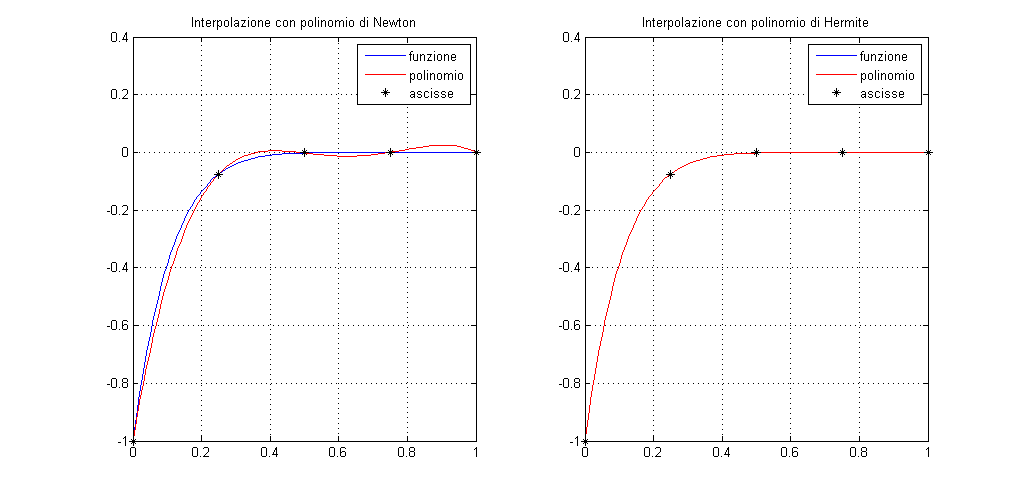
\includegraphics[scale=0.45]{es4_9a.png}
			\end{center}
			\begin{center}
				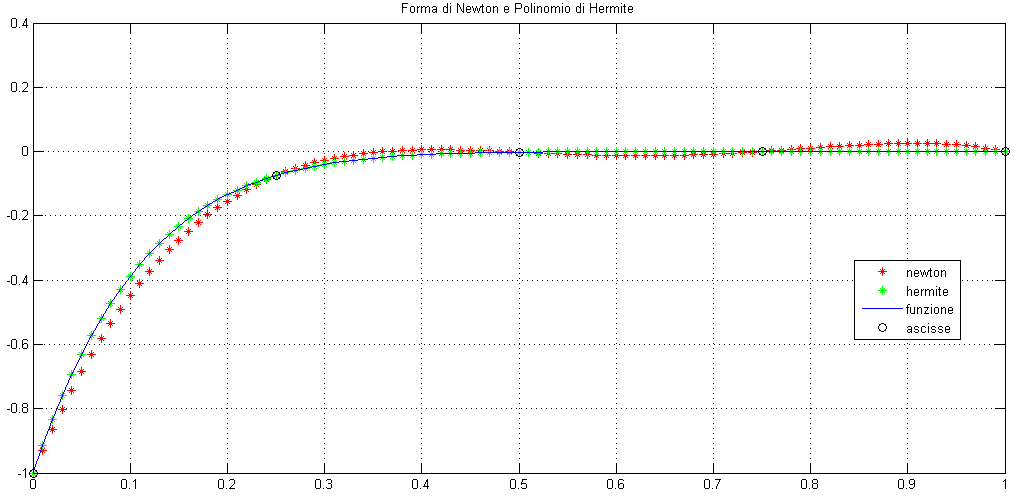
\includegraphics[scale=0.45]{es4_9b.png}
			\end{center}
			Dai grafici ottenuti si vede che l'interpolazione tramite polinomio di Newton approssima abbastanza bene la funzione, mentre utilizzando il polinomio di Hermite si ha una totale coincidenza tra la funzione originaria ed il polinomio interpolante. Questo � dovuto al fatto che il polinomio di Hermite interpola la funzione su un totale di $10$ ascisse, il che lo rende a tutti gli effetti un polinomio di grado $9$, esattamente come la funzione originaria. Il polinomio di newton, invece, interpolando la funzione su $5$ sole ascisse, risulta essere un polinomio di quarto grado.
			\begin{flushright}
				\underline{Riferimenti \textsc{Matlab}}\\
				Codice \ref{lst:es4.9} (pagina \pageref{lst:es4.9})
			\end{flushright}
		\end{sol}
		\sectionline
		\begin{es} %4.10
			\label{es:4.10}
			Quante ascisse di interpolazione equidistanti sono necessarie per approssimare la funzione $\sin(x)$ sull'intervallo $[0,2\pi]$, con un errore di interpolazione inferiore a $10^{-6}$?
		\end{es}
		\begin{sol}
			\normalfont Considerando l'espressione dell'errore d'interpolazione (\ref{erroreInterpolazione}) si pu� massimizzare $\left|f^{(n+1)}(\xi_x)\right|\leq 1$ in quando le derivate di $f(x)$ sono $\pm\sin{x}$, $\pm\cos{x}$ quindi limitate; inoltre $w_{n+1}(x)=\prod_{j=0}^{n}{(x-x_j)}\leq\prod_{j=0}^{n}{2\pi}=2\pi^{n+1}$ poich� $|x-x_j|\leq 2\pi$, $\forall j$. Segue $e(x)=\frac{1}{(n+1)!}(2\pi)^{n+1}$; eseguendo lo script \textsc{Matlab}, risulta \texttt{e(26) = 3.265e-007}$\leq 10^{-6}$.
			\begin{flushright}
				\underline{Riferimenti \textsc{Matlab}}\\
				Codice \ref{lst:es4.10} (pagina \pageref{lst:es4.10})
			\end{flushright}
		\end{sol}
		\sectionline
		\begin{es} %4.11
			\label{es:4.11}
			Verificare sperimentalmente che, considerando le ascisse di interpolazione equidistanti (\ref{ascisseEquidistanti}) su cui si definisce il polinomio $p(x)$ interpolante $f(x)$, l'errore $||f-p||$ diverge, al crescere di $n$, nei seguenti due casi:
			\begin{enumerate}
				\item esempio di Runge:
					$$f(x)=\frac{1}{1+x^2},\qquad [a,b]\equiv[-5,5];$$
				\item esempio di Bernstein:
					$$f(x)=|x|,\qquad [a,b]\equiv[-1,1].$$
			\end{enumerate}
		\end{es}
		\begin{sol}
			\begin{itemize}
				\item \underline{Esempio di Runge:}\\
					Osserviamo i seguenti grafici che mostrano, rispettivamente, l'errore commesso con $n=5,10,15$ e l'interpolazione della funzione per $n=5,10,15,20$:
					\begin{center}
						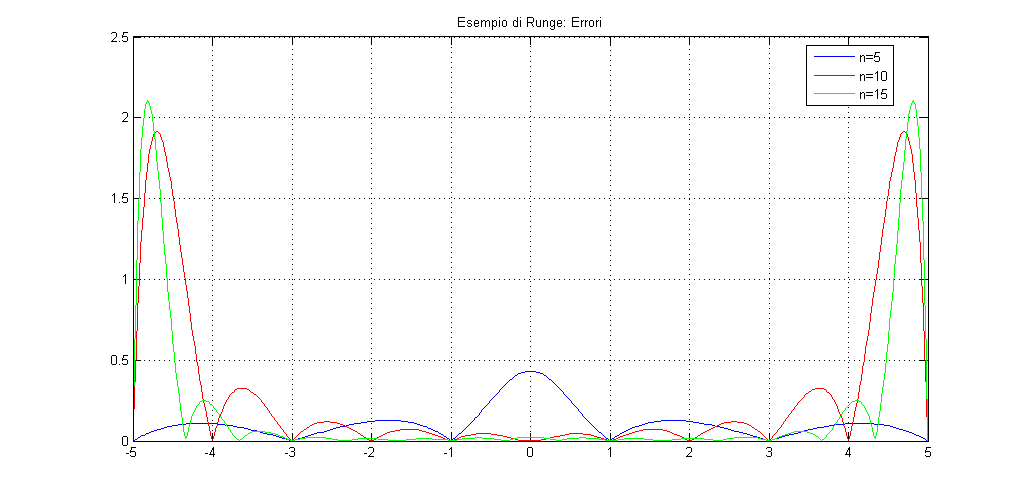
\includegraphics[scale=0.4]{es4_11a.png}
					\end{center}
					\begin{center}
						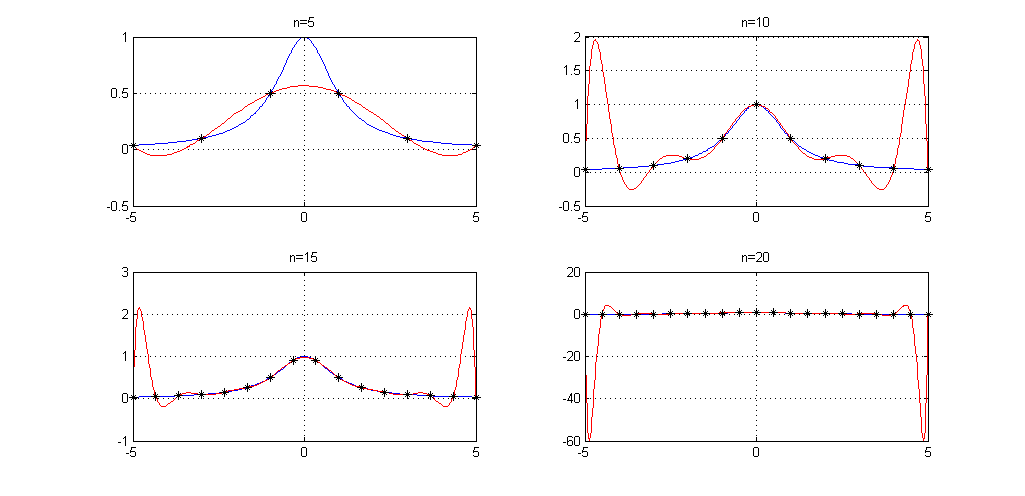
\includegraphics[scale=0.4]{es4_11b.png}
					\end{center}
				\item \underline{Esempio di Bernstein:}
					Come per l'esempio di Runge, proponiamo i grafici dell'errore e dell'interpolazione per l'esempio di Bernstein:
					\begin{center}
						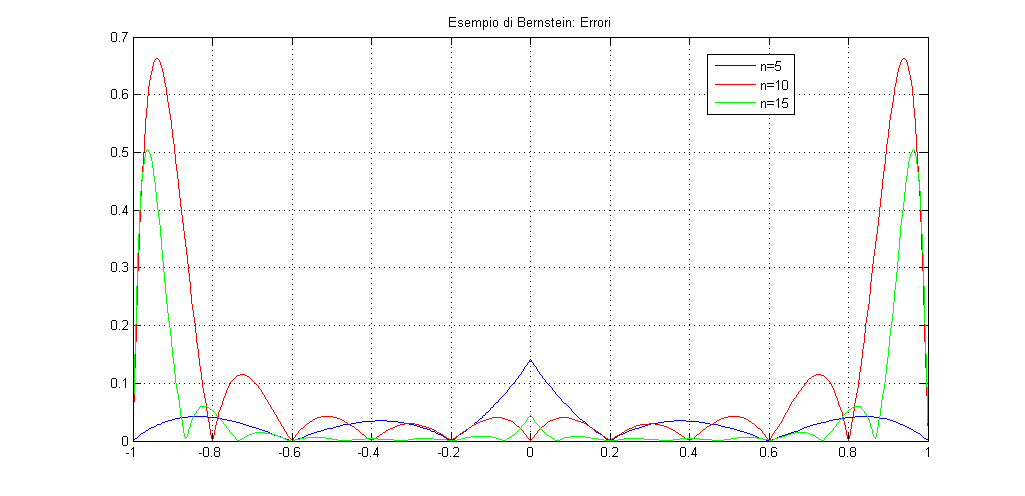
\includegraphics[scale=0.4]{es4_11c.png}
					\end{center}
					\begin{center}
						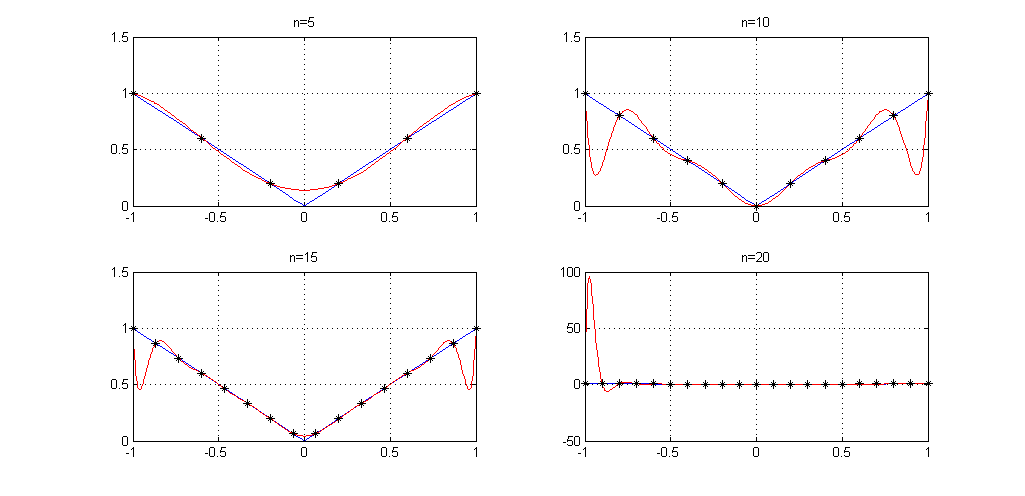
\includegraphics[scale=0.4]{es4_11d.png}
					\end{center}
			\end{itemize}
			Da i grafici proposti per le due funzioni d'esempio deduciamo che l'errore commesso tende a divergere all'aumentare di $n$ con le ascisse di interpolazione scelte equidistanti, ovvero uniformemente distribuite sull'intervallo di interpolazione. Vediamo infine i valori dell'errore massimo di interpolazione commesso nei due esempi per $n=5,10,15,20$:
			\begin{center}
				\begin{tabular}{c||c|c}
					\multirow{2}{*}{$n$} & \multicolumn{2}{|c}{\textbf{Errore}}\\
					& \textbf{Runge} & \textbf{Bernstein}\\
					\hline
					$5$ & 0.4327 & 0.0422\\
					$10$ & 0.3276 & 0.1149\\
					$15$ & 2.1076 & 0.5054\\
					$20$ & 59.8223 & 95.1889
				\end{tabular}
			\end{center}
			\begin{flushright}
				\underline{Riferimenti \textsc{Matlab}}\\
				Codice \ref{lst:es4.11} (pagina \pageref{lst:es4.11})
			\end{flushright}
		\end{sol}
		\sectionline
		\begin{es} %4.12
			\label{es4.12}
			Dimostrare che, se $x\in[-1,1]$, allora:
			$$\tilde{x}\equiv\frac{a+b}{2}+\frac{b-a}{2}x\in[a,b].$$
			Viceversa, se $\tilde{x}\in[a,b]$, allora:
			$$x\equiv\frac{2\tilde{x}-a-b}{b-1}\in[-1,1].$$
			Concludere che � sempre possibile trasformare il problema di interpolazione (\ref{ascisse})-(\ref{condizioniInterp}) in uno definito sull'intervallo $[-1,1]$, e viceversa.
		\end{es}
		\begin{sol}
			\normalfont
			\begin{itemize}
				\item $x\in[-1,1]\:\Rightarrow\:\tilde{x}\in[a,b]$:
			\begin{itemize}
				\item se $x=-1$, $\tilde{x}=\frac{a+b}{2}-\frac{b-a}{2} = a$;
				\item se $x=1$, $\tilde{x}=\frac{a+b}{2}+\frac{b-a}{2} = b$.
			\end{itemize}
				\item $\tilde{x}\in[a,b]\:\Rightarrow\:x\in[-1,1]$:
			\begin{itemize}
				\item se $\tilde{x}=a$, $x=\frac{2a-a-b}{b-a}=-1$;
				\item se $\tilde{x}=b$, $x=\frac{2b-a-b}{b-a}=1$;
			\end{itemize}
			\end{itemize}
		\end{sol}
		\sectionline
		\begin{es} %4.13
			Dimostrare le propriet� dei polinomi di Chebyshev di I specie (\ref{chebyshevISpecie}) elencate nel Teorema \ref{propriet�PolinomiChebyshev}.
		\end{es}
		\begin{sol}
			\normalfont
			Prime propriet�
			\begin{enumerate}
				\item $T_k(x)$ � un polinomio di grado esatto $k$:
			\begin{itemize}
				\item $k=0$: $T_0(x)=1$ polinomio di grado $0$;
				\item $k>0$: $T_{k+1}(x)=2xT_k(x)-T_{k-1}(x)$ dove, per ipotesi induttiva, $T_k(x)$ � un polinomio di grado $k$ quindi $T_{k+1}(x)$ � un polinomio di grado $k+1$.
			\end{itemize}
				\item Il coefficiente principale di $T_k(x)$ � $2^{k-1}$, $k=1,2,\ldots$:
				\begin{itemize}
				\item $k=1$: $T_1(x)=x$ e $2^{1-1}=1$;
				\item $k>1$: $T_{k+1}(x)=2xT_k(x)-T_{k-1}(x)$ dove, per ipotesi induttiva, il coefficiente principale di $T_k(x)$ � $2^{k-1}$ quindi il coefficiente principale di $T_{k+1}(x)$ � $2\cdot2^{k-1}=2^k$.
			\end{itemize}
				\item La famiglia di polinomi $\{\hat{T}_k\}$, in cui $$\hat{T}_0(x)=T_0(x),\quad\hat{T}_k(x)=2^{1-k}T_k(x),\quad k=1,2,\ldots,$$ � una famiglia di polinomi monici di grado $k$, $k=1,2,\ldots$:
			\begin{itemize}
				\item grado $k$: il grado di $\hat{T}_k$ coincide con il grado di $T_k(x)$ che � $k$;
				\item monici: il coefficiente principale di $\hat{T}_k$ � $2^{1-k}$ dunque $2^{1-k}2^{k-1}=1$ il polinomio � monico.
			\end{itemize}
				\item Ponendo $x=\cos{\theta}$, $\theta\in[0,\pi]$, si ottiene $T_k(x)=T_k(\cos{\theta})=\cos{k\theta},\quad k=0,1,\ldots$:
			\begin{itemize}
				\item $k=0$: $T_0(\cos{\theta})=\cos{0\theta}=1=T_0(x)$;
				\item $k=1$: $T_0(\cos{\theta})=\cos{\theta}=x=T_1(x)$:
				\item $k>1$: $T_{k+1}(\cos{\theta})=2\cos{\theta}T_k({\cos{\theta}})-T_{k-1}(\cos{\theta})$ per ipotesi induttiva, $T_k({\cos{\theta}})=\cos{k\theta}$ e $T_{k-1}(\cos{\theta})=\cos{(k-1)\theta}$ dunque $T_{k+1}(\cos{\theta})=2\cos{\theta}\cos{k\theta}-\cos{(k-1)\theta}=\cos{(k+1)\theta}+\cos{(k-1)\theta}-\cos{(k-1)\theta}=\cos{(k+1)\theta}=T_{k+1}(x)$.
			\end{itemize}
			\end{enumerate}
			Teorema 4.9
			\begin{itemize}
				\item Radici del polinomio: $T_k(x)=T_k(\cos{\theta})=\cos{k\theta}=0$ se $\cos{k\theta}=0$ ovvero per $k\theta=\frac{\pi}{2}+i\pi$; segue $\theta_i=\frac{\frac{\pi}{2}+i\pi}{k}=\frac{(2i+1)\pi}{2k}$ cio� gli zeri del polinomio sono dati da $x_i^{(k)}=\cos{\frac{(2i+1)\pi}{2k}}$.
				\item Estremi: Agli estremi $\cos{k\theta}=\pm 1$ ovvero $k\theta=i\pi$; segue $\theta_i=\frac{i}{k}\pi$ dunque gli estremi sono assunti in $\xi_i^{(k)}=\cos{\frac{i}{k}\pi}$; in tali punti, poich� $\cos{k\pi}=(-1)^i$ la funzione vale $T_k(\xi_i^{(k)})=(-1)^i$.
				\item Norme: dal punto precedente segue inoltre $||T_k||=1$ e  $||\hat{T}_k||=||2^{1-k}T_k||=||2^{1-k}||$.
				\item Minima norma per $\hat{T}_k(x)$: supponiamo per assurdo che $\exists p\neq\hat{T}_k(x)$ monico tale che $||p||<2^{1-k}=||\hat{T}_k||$, quindi $g(x)=\hat{T}_k-p(x)\in\Pi_{k-1}$ poich� entrambi monici di grado $K$. Studiando il segno di $g$ si nota $sign(g(x_i))=(-1)^i$ per $i=0,\ldots,k$ ovvero ci sono $k$ cambiamenti di segno quindi $k$ radici cio� $g(x)\in\Pi_k$ ma, per ipotesi, $g(x)\in\Pi_{k-1}$ quindi $g(x)=0$.
			\end{itemize}
		\end{sol}
		\sectionline
		\begin{es} %4.14
			Quali diventano le ascisse di Chebyshev (\ref{ascisseChebyshev}), per un problema definito su un generico intervallo $[a,b]$?
		\end{es}
		\begin{sol}
			\normalfont Le ascisse di Chebyshev sono $$x_{n-i}=\cos{\frac{(2i+1)\pi}{2(n+1)}}\in[-1,1];$$ utilizzando il risultato dell'Esercizio 4.12 si ha $$\tilde{x}_{n-i}=\frac{a+b}{2}-\frac{b-a}{2}\cos{\frac{(2i+1)\pi}{2(n+1)}}\in[a,b].$$Tali $\tilde{x}_i$ definiscono le ascisse di Chebyshev per un generico intervallo $[a,b]$.
		\end{sol}
		\sectionline
		\begin{es} %4.15
			\label{es:4.15}
			Utilizzare le ascisse di Chebyshev (\ref{ascisseChebyshev}) per approssimare gli esempi visti nell'Esercizio \ref{es:4.11}, per $n=2,4,6,\dots,40$.
		\end{es}
		\begin{sol}
			Similmente a quanto visto nell'Esercizio \ref{es:4.11} mostriamo di seguito i grafici degli errori e di interpolazione per $n=5,10,15,20$, rispetto agli esempi di Runge e Bernstein.
			\begin{itemize}
				\item \underline{Esempio di Runge}:
					\begin{center}
						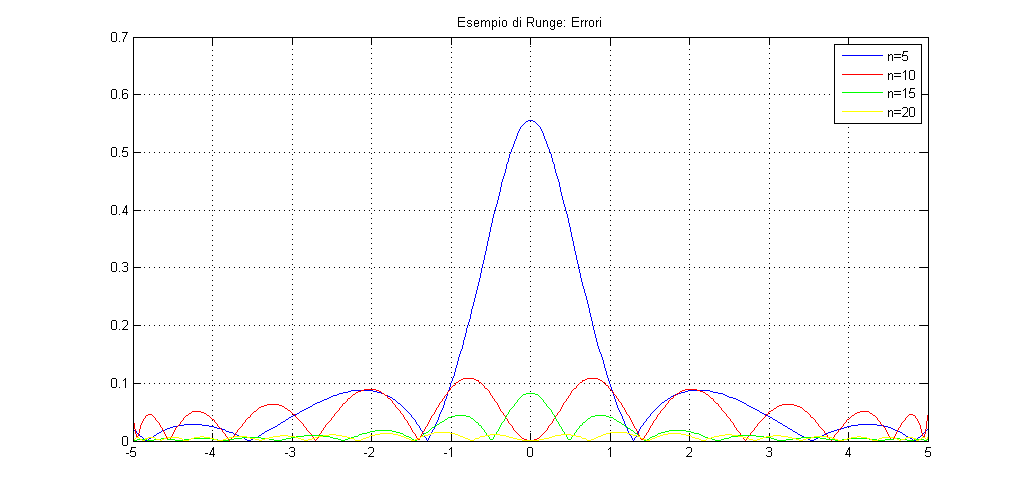
\includegraphics[scale=0.4]{es4_15a.png}
					\end{center}
					\begin{center}
						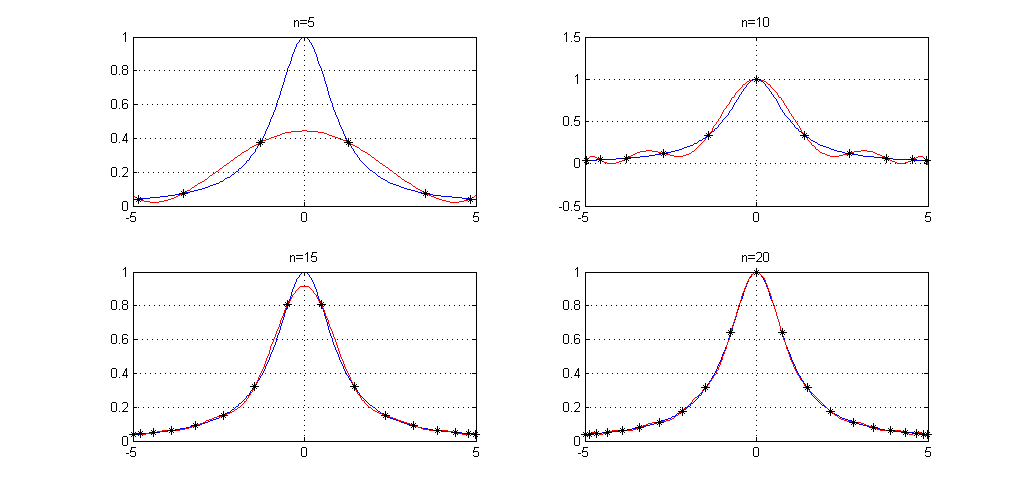
\includegraphics[scale=0.4]{es4_15b.png}
					\end{center}
				\item \underline{Esempio di Bernstein}:
					\begin{center}
						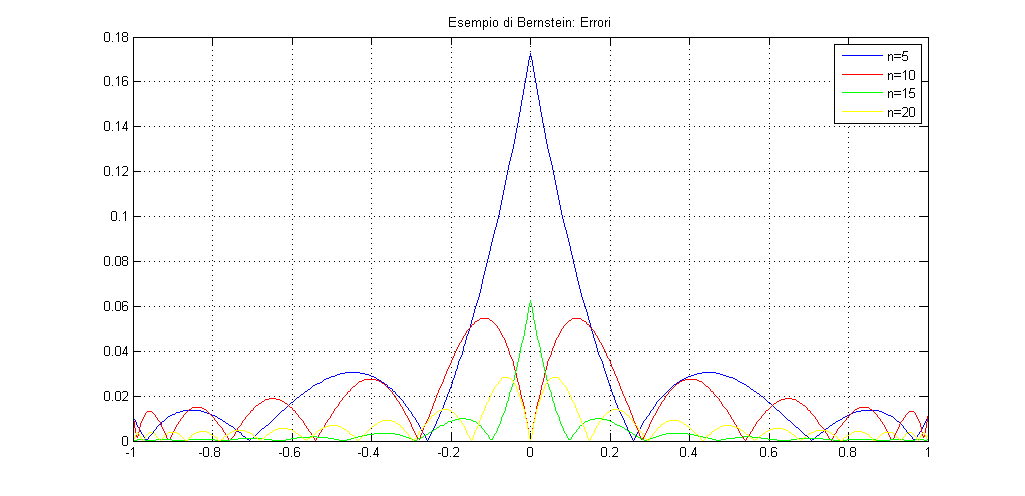
\includegraphics[scale=0.4]{es4_15c.png}
					\end{center}
					\begin{center}
						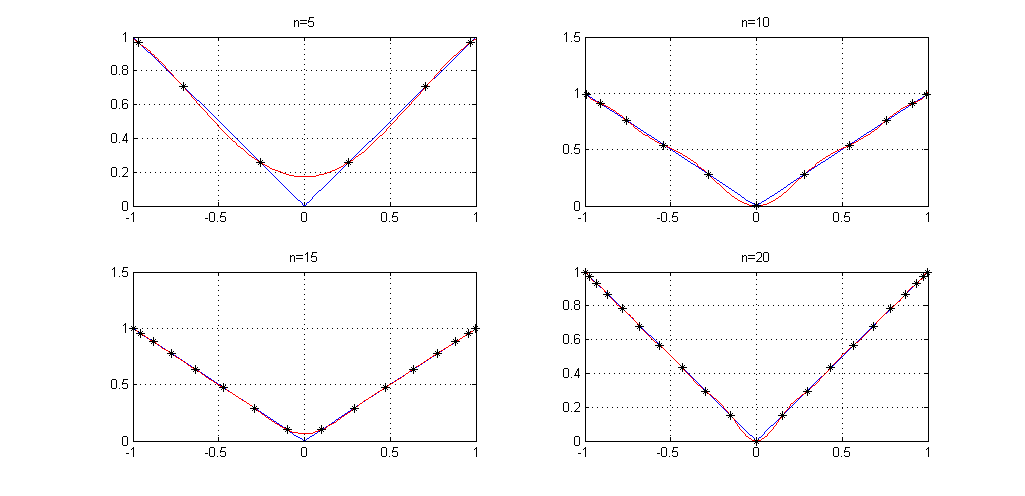
\includegraphics[scale=0.4]{es4_15d.png}
					\end{center}
			\end{itemize}
			Di seguito proponiamo anche gli errori di interpolazione massimi commessi nei due esempi per $n=5,10,15,20$:
			\begin{center}
				\begin{tabular}{c||c|c}
					\multirow{2}{*}{$n$} & \multicolumn{2}{|c}{\textbf{Errore}}\\
					& \textbf{Runge} & \textbf{Bernstein}\\
					\hline
					$5$ & 0.0881 & 0.0305\\
					$10$ & 0.0897 & 0.0275\\
					$15$ & 0.0831 & 0.0628\\
					$20$ & 0.0153 & 0.0140
				\end{tabular}
			\end{center}
			Si evince quindi, dai grafici e dai valori riportati, che la scelta delle ascisse di Chebyshev al posto di ascisse equidistanti � estremamente pi� conveniente, in quanto evita la divergenza dell'errore di interpolazione all'aumentare di $n$. Infatti l'errore commesso, all'aumentare di $n$ risulta essere in generale molto stabile e, molto spesso, risulta anche in diminuzione.
			\begin{flushright}
				\underline{Riferimenti \textsc{Matlab}}\\
				Codice \ref{lst:es4.15} (pagina \pageref{lst:es4.15})
			\end{flushright}
		\end{sol}
		\sectionline
		\begin{es} %4.16
			\label{es:4.16}
			Verificare che la fattorizzazione $LU$ della matrice dei coefficienti del sistema tridiagonale (\ref{sistemaSplineNaturale}) � dato da:
			\[
				L=
				\begin{pmatrix}
					1 & & &\\
					l_2 & 1 & &\\
					& \ddots & \ddots &\\
					& & l_{n-1} & 1
				\end{pmatrix},
				\qquad U=
				\begin{pmatrix}
					u_1 & \xi_1 & &\\
					& u_2 & \ddots &\\
					& & \ddots & \xi_{n-2}\\
					& & & u_{n-1}
				\end{pmatrix},
			\]
			con
			\begin{align*}
				&u_1=2,\\
				&l_i=\frac{\varphi_i}{u_{i-1}},\\
				&u_i=2-l_i\xi_{i-1},\qquad i=2,\dots,n-1.
			\end{align*}
			Scrivere una \lstinline{function} \textsc{Matlab} che implementi efficientemente la risoluzione della (\ref{sistemaSplineNaturale}).
		\end{es}
		\begin{sol}
			La matrice dei coefficienti
			\[
				A=\begin{pmatrix}
					2 & \xi_1 & & &\\
					\varphi_2 & 2 & \xi_2 & &\\
					& \ddots & \ddots & \ddots &\\
					& & \ddots & \ddots & \xi_{n-2}\\
					& & & \varphi_{n-1} & 2
				\end{pmatrix}
			\]
			si vede essere \textit{dominante per righe} in quanto, essendo
			$$\varphi_i=\frac{h_i}{h_i+h_{i+1}},\qquad\xi_i=\frac{h_{i+1}}{h_i+h_{i+1}},\qquad i=1,\dots,n-1,$$
			si vede facilmente che $\varphi_i+\xi_i=1$. Quindi la matrice � fattorizzabile $LU$.\\
			Moltiplichiamo adesso i termini $L$ ed $U$ e vediamo che il risultato sono proprio i termini della matrice $A$:
			\begin{itemize}
				\item $a_{11}=1\cdot u_1=u_1=2$;
				\item $a_{12}=1\cdot\xi_1 + 0\cdot u_2=\xi_1$;
				\item $a_{i,i-1}=0\cdot\xi_{i-2}+l_i\cdot u_{i-1}+1\cdot 0=l_i\cdot u_{i-1}=\frac{\varphi_i}{u_{i-1}}u_{i-1}=\varphi_i$, per $i>1$;
				\item $a_{ii}=l_i\cdot\xi_{i-1}+1\cdot u_i=l_i\xi_{i-1}+2-l_i\xi_{i-1}=2$, per $i>1$;
				\item $a_{i,i+1}=l_i\cdot 0+1\cdot\xi_i +0\cdot u_{i+1}=\xi_i$, per $i>1$.
			\end{itemize}
			Quindi il sistema $A\underline{m}=\underline{d}$ si risolve come segue:
			\begin{itemize}
				\item si risolve $L\underline{y}= 6\underline{d}$:
					\begin{itemize}
						\item $y_1=6d_1$,
						\item $y_i=6d_i-l_iy_{i-1}$ per $i=2,\dots,n-1$;
					\end{itemize}
				\item si risolve il sistema $U\underline{m}=\underline{y}$:
					\begin{itemize}
						\item $m_{n-1}=\frac{y_{n-1}}{u_{n-1}}$,
						\item $m_{i}=\frac{y_i-\xi_i m_{i+1}}{u_i}$, per $i=n-2, \dots ,1$.
					\end{itemize}
			\end{itemize}
			Per quanto riguarda l'implementazione \textsc{Matlab} dell'algoritmo per la risoluzione di suddetto sistema lineare, fare riferimento al Codice \ref{lst:risolviSistemaSplineNaturale} a pagina \pageref{lst:risolviSistemaSplineNaturale}. In questa implementazione si � deciso di non utilizzare la fattorizzazione $LU$ vista in Sezione \ref{sez3.2} (la cui implementazione in \textsc{Matlab} � consultabile a pagina \pageref{lst:fattorizzaLU}), ma se ne propone una versione ottimizzata basata sulle osservazioni appena fatte.
		\end{sol}
		\sectionline
		\begin{es} %4.17
			\label{es:4.17}
			Generalizzare la fattorizzazione del precedente Esercizio \ref{es:4.16} al caso della matrice dei coefficienti del sistema lineare (\ref{sistemaSplineNaK}). Scrivere una corrispondente \lstinline{function} \textsc{Matlab} che risolva efficientemente questo sistema.
		\end{es}
		\begin{sol}
			Generalizzando il risultato ottenuto nell'Esercizio \ref{es:4.16}, la fattorizzazione � della forma
			\[
				L=\begin{pmatrix}
					1 & & &\\
					l_2 & 1 & &\\
					& \ddots & \ddots &\\
					& & l_{n+1} & 1
				\end{pmatrix},\qquad U=\begin{pmatrix}
					u_1 & w_1 & &\\
					& u_2 & \ddots &\\
					& & \ddots & w_n\\
					& & & u_{n+1}
				\end{pmatrix}.
			\]
			Se come prima moltiplichiamo i fattori $L$ ed $U$ ricaviamo le espressioni degli $l_i$, $u_i$ e $w_i$:
			\begin{itemize}
				\item per $i=4,\dots,n-1$:
					\[
						\begin{cases}
							u_i=2-l_iw_{i-1}\\
							w_{i-1}=\xi_{i-2}\\
							l_i=\frac{\varphi_{i-1}}{u_{i-1}}
						\end{cases};
					\]
				\item per $i=3$:
					\[
						\begin{cases}
							u_3=2-l_3w_2\\
							w_2=\xi_1-\varphi_1\\
							l_3=\frac{\varphi_2}{u_2}
						\end{cases};
					\]
				\item per $i=2$:
					\[
						\begin{cases}
							u_2=2-\varphi_1\\
							w_1=0\\
							l_2=\frac{\varphi_1}{u_1}
						\end{cases};
					\]
				\item per $i=1$:
					$$u_1=1;$$
				\item per $i=n$:
					\[
						\begin{cases}
							u_n=2-\xi_{n-1}-l_nw_{n-1}\\
							w_{n-1}=\xi_{n-2}\\
							l_n=\frac{\varphi_{n-1}-\xi_{n-1}}{u_{n-1}}
						\end{cases};
					\]
				\item per $i=n+1$:
					\[
						\begin{cases}
							u_{n+1}=1\\
							w_n=\xi_{n-1}\\
							l_{n+1}=0
						\end{cases}
					\].
			\end{itemize}
			Quindi come prima avremo:
			\begin{itemize}
				\item risoluzione del sistema $L\underline{y}= 6\underline{d}$:
					\begin{itemize}
						\item $y_1=6d_1$,
						\item $y_i=6d_i-l_iy_{i-1}$ per $i=2,\dots,n+1$;
					\end{itemize}
				\item risoluzione del sistema $U\underline{\hat{m}}=\underline{y}$:
					\begin{itemize}
						\item $\hat{m}_{n+1}=\frac{y_{n+1}}{u_{n+1}}$,
						\item $\hat{m}_{i}=\frac{y_i-w_i \hat{m}_{i+1}}{u_i}$, per $i=n, \dots ,1$;
					\end{itemize}
				\item calcolo della soluzione:
					\begin{itemize}
						\item $m_1=\hat{m}_1-\hat{m}_2-\hat{m}_3$,
						\item $m_i=\hat{m}_i$, per $i=2,\dots,n$,
						\item $m_{n+1}=\hat{m}_{n+1}-\hat{m}_n-\hat{m}_{n-1}$.
					\end{itemize}
			\end{itemize}
			Per l'implementazione in \textsc{Matlab} della \lstinline{function} relativa, si veda il Codice \ref{lst:risolviSistemaSplineNotAKnot} a pagina \pageref{lst:risolviSistemaSplineNotAKnot}.
		\end{sol}
		\sectionline
		\begin{es} %4.18
			Scrivere una \lstinline{function} \textsc{Matlab} che, noti gli $\{m_i\}$ in (\ref{mi}), determini l'espressione, polinomiale a tratti, della spline cubica (\ref{espressioneSpline}).
		\end{es}
		\begin{sol}
			Per l'implementazione \textsc{Matlab} dell'algoritmo che determina l'espressione polinomiale a tratti di una spline cubica si veda il Codice \ref{lst:espressioniSplineCubica} a pagina \pageref{lst:espressioniSplineCubica}. In questo algoritmo viene creato un vettore contenente le espressioni degli $n$ polinomi che definiscono la spline cubica, applicando la (\ref{espressioneSpline}), passando come input i nodi di interpolazione, i valori assunti dalla funzione in tali nodi e i fattori $m_i$, eventualmente calcolati utilizzando gli Algoritmi degli Esercizi \ref{es:4.16} e \ref{es:4.17}.
		\end{sol}
		\sectionline
		\begin{es} %4.19
			\label{es4.19}
			Costruire una \lstinline{function} \textsc{Matlab} che implementi le spline cubiche naturali e quelle definite dalle condizioni not-a-knot.
		\end{es}
		\begin{sol}
			Per l'implementazione si veda il Codice \ref{lst:splineCubica} a pagina \pageref{lst:splineCubica}, nel quale la scelta tra spline naturale e con condizioni not-a-knot dipende dal valore dell'input \lstinline{nak} (rispettivamente, false e true). Quello che viene fatto � creare, a partire dai nodi di interpolazione e dai valori assunti dalla funzione in tali punti, i vettori $\underline{\varphi}$, $\underline{\xi}$ e delle differenze divise (si � costruita una nuova \lstinline{function} che calcola una singola differenza divisa in modo indipendente dalle altre, in quanto la \lstinline{function} che era stata scritta per la forma di Newton non � chiaramente riutilizzabile). Viene quindi risolto il sistema lineare corrispondente per determinare i fattori $m_i$ ed infine viene determinata l'espressione della spline, ovvero le espressioni degli $n$ polinomi costituenti la spline cubica. � stata scritta, inoltre, una \lstinline{function} \textsc{Matlab} che, prendendo in input i nodi di interpolazione, l'espressione della spline ed un set di punti, restituisce la valutazione della spline in corrispondenza di tali punti.
		\end{sol}
		\sectionline
		\begin{es} %4.20
			\label{es:4.20}
			Utilizzare la \lstinline{function} dell'Esercizio \ref{es4.19} per approssimare, su partizioni (\ref{partizione}) uniformi con $n=10,20,30,40$, gli esempi proposti nell'Esercizio \ref{es:4.11}.
		\end{es}
		\begin{sol}
			I grafici ottenuti mostrano l'interpolazione delle due funzioni d'esempio tramite spline cubiche con condizioni \textit{not-a-knot} (si osservi che nei grafici i due punti definiti, appunto, \textit{not-a-knot}, sono indicati da un cerchio nero al posto di un asterisco come per tutti gli altri nodi). Non sono stati riportati i grafici riguardanti l'interpolazione tramite spline cubiche naturali in quanto tra i due tipi di grafici non sono presenti sostanziali differenze (eseguendo il file \textsc{Matlab} relativo vengono disegnati entrambi i grafici per i due esempi).
			\begin{itemize}
				\item \underline{Esempio di Runge}:
					\begin{center}
						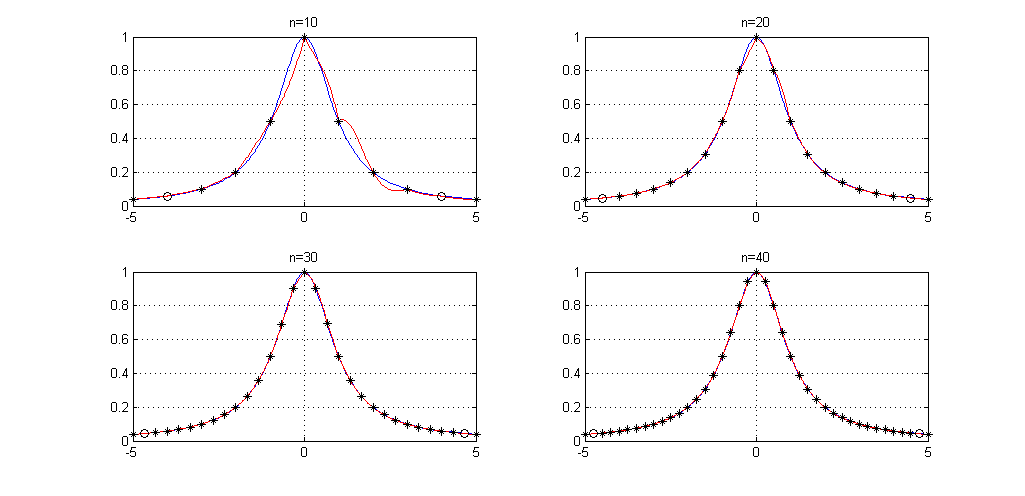
\includegraphics[scale=0.4]{es4_20a.png}
					\end{center}
				\item \underline{Esempio di Bernstein}:
					\begin{center}
						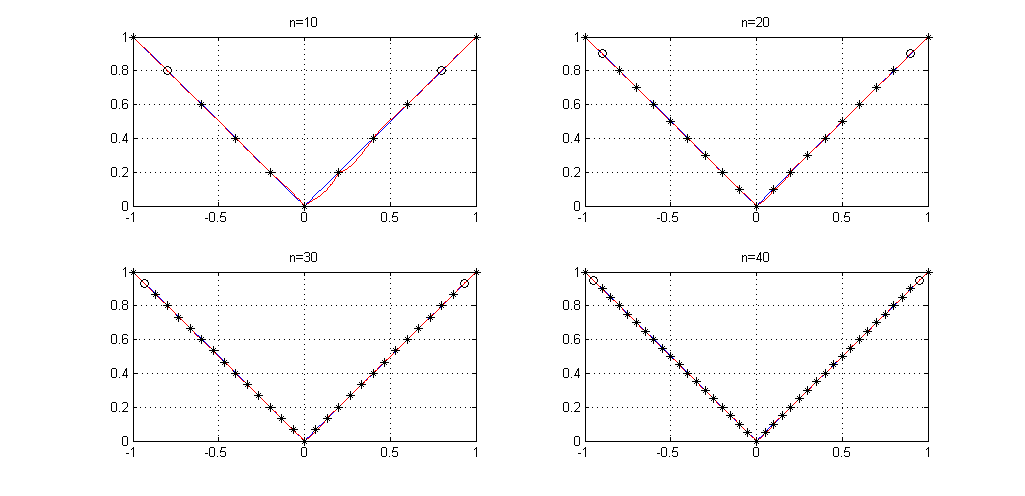
\includegraphics[scale=0.4]{es4_20b.png}
					\end{center}
			\end{itemize}
			\begin{flushright}
				\underline{Riferimenti \textsc{Matlab}}\\
				Codice \ref{lst:es4.20} (pagina \pageref{lst:es4.20})
			\end{flushright}
		\end{sol}
		\sectionline
		\begin{es} %4.21
			Interpretare la retta dell'Esercizio \ref{es:3.32} come retta di approssimazione ai minimi quadrati dei dati.
		\end{es}
		\begin{sol}
			\normalfont Il problema ai minimi quadrati � dato da $$\min_{a_1,a_2\in\mathbb{R}}{\sum_{k=0}^n{|y_i-a_1x_i-a_2|^2}}$$ dove $\underline{y}$ � il vettore dei valori previsti per la retta. Il problema � esprimibile in forma matriciale come $$\begin{pmatrix}1&x_0\\1&x_1\\\vdots&\vdots\\1&x_n\end{pmatrix}\begin{pmatrix}a_2\\a_1\end{pmatrix}=\begin{pmatrix}y_0\\y_1\\\vdots\\y_n\end{pmatrix} ;$$ si tratta di risolvere un sistema sovradeterminato che ha soluzione se almeno $2$ ascisse sono distinte in quanto $r(x)\in\Pi_1$.
		\end{sol}
		\sectionline
		\begin{es} %4.22
			\label{es:4.22}
			� noto che un fenomeno ha un decadimento esponenziale, modellizzato come
			$$y=\alpha\cdot e^{-\lambda t},$$
			in cui $\alpha$ e $\lambda$ sono parametri positivi e incogniti. Riformulare il problema in modo che il modello sia di tipo polinomiale. Supponendo inoltre di disporre delle seguenti misure,
			\begin{center}
				\setlength{\tabcolsep}{4pt}
				\begin{tabular}{|c|c c c c c c c c c c c|}
					\hline
					$t_1$ & 0 & 1 & 2 & 3 & 4 & 5 & 6 & 7 & 8 & 9 & 10\\
					\hline
					$y_i$ & 5.22 & 4.00 & 4.28 & 3.89 & 3.53 & 3.12 & 2.73 & 2.70 & 2.20 & 2.08 & 1.94\\
					\hline
				\end{tabular}
			\end{center}
			calcolare la stime ai minimi quadrati dei due parametri incogniti. Valutare il residuo e raffigurare, infine, i risultati ottenuti.
		\end{es}
		\begin{sol}
			\normalfont 
			Il problema in forma polinomiale � $$\bar{y}=\bar{\alpha}+\bar{\lambda}t,\quad\mbox{ con }\bar{y}=\log{y}\mbox{, }\bar{\alpha}=\log{\alpha}\mbox{ e }\bar{\lambda}=-\lambda$$ infatti si ha $y=\alpha\cdot e^{-\lambda t}\:\Rightarrow\:\log{y}=\log{(\alpha\cdot e^{-\lambda t})}\:\Rightarrow\:\log{y}=\log{\alpha}-\lambda t\:\:\Rightarrow\:\bar{y}=\bar{\alpha}+\bar{\lambda}t$. Si tratta di risolvere il sistema lineare sovradeterminato $$\begin{pmatrix}1&t_0\\1&t_1\\\vdots&\vdots\\1&t_10\end{pmatrix}\begin{pmatrix}\bar{\alpha}\\\bar{\lambda}\end{pmatrix}=\begin{pmatrix}\bar{y}_0\\\bar{y}_1\\\vdots\\\bar{y}_n\end{pmatrix}$$ 
			mediante fattorizzazione $QR$ (possibile poich� tutte le ascisse sono distinte) e ricavare $\begin{pmatrix}\bar{\alpha}\\\bar{\lambda}\end{pmatrix}$ da qui $\begin{pmatrix}\alpha\\\lambda\end{pmatrix}=\begin{pmatrix}e^{\bar{\alpha}}\\-\bar{\lambda}\end{pmatrix}.$\\I risultati ottenuti dallo \lstinline{scritp} \textsc{Matlab} sono $\begin{pmatrix}\alpha\\\lambda\end{pmatrix}=\begin{pmatrix}5.008\\0.0959\end{pmatrix}$ con un residuo $r=0.1708$. \centering\begin{figure}[H]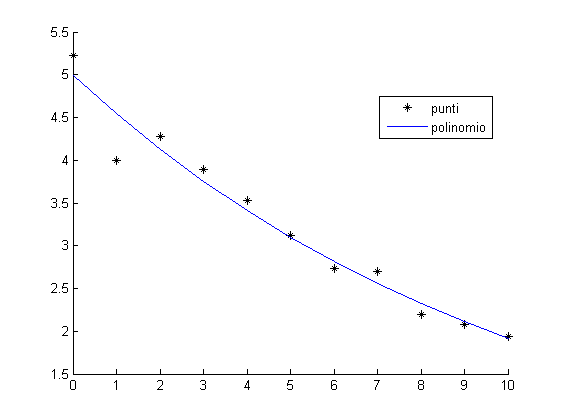
\includegraphics[scale=0.60]{es4_22.png}\end{figure}
			\begin{flushright}
				\underline{Riferimenti \textsc{Matlab}}\\
				Codice \ref{lst:es4.22} (pagina \pageref{lst:es4.22})
			\end{flushright}
		\end{sol}
	\section*{Codice degli esercizi}
		\addcontentsline{toc}{section}{Codice degli esercizi}
		\markboth{\textsc{\uppercase{Capitolo }\ref{chapterApprossimazioniFunzioni}\uppercase{. Approssimazione di funzioni}}}{\textsc{\uppercase{Codice degli esercizi}}}
		\lstinputlisting[caption={Esercizio \ref{es:4.9}.}, label=lst:es4.9]{code/es4_9.m}
		\sectionline
		\lstinputlisting[caption={Esercizio \ref{es:4.10}.}, label=lst:es4.10]{code/es4_10.m}
		\sectionline
		\lstinputlisting[caption={Esercizio \ref{es:4.11}.}, label=lst:es4.11]{code/es4_11.m}
		\sectionline
		\lstinputlisting[caption={Esercizio \ref{es:4.15}.}, label=lst:es4.15]{code/es4_15.m}
		\sectionline
		\lstinputlisting[caption={Esercizio \ref{es:4.20}.}, label=lst:es4.20]{code/es4_20.m}
		\sectionline
		\lstinputlisting[caption={Esercizio \ref{es:4.22}.}, label=lst:es4.22]{code/es4_22.m}
		
	\chapter{Predizione della prossima alta marea}
	Oltre alla predizione dopo un numero fissato di ore un altro importante esperimento è quello della predizione del prossimo picco di alta marea. Come nei capitoli precedenti, la chiocciola osserva \textbf{5} altezze di marea, ad \textbf{1 ora} di distanza ciascuna, per poi predire sia tra quante ore avverrà la prossima alta marea, sia l'altitudine che raggiungerà.\\
	Per quanto riguarda gli errori sensoriali a cui la chiocciola può essere soggetta si è deciso di mantenere il \textbf{15\%} di errore sulla percezione del livello dell'acqua e del \textbf{16\%} sulla percezione del trascorrere del tempo che, essendo in questo caso l'intervallo tra due osservazioni successive di un'ora, corrisponde a \textbf{\(\pm\) 10 minuti}.
	\section{Predizione con rete lineare di Widrow}
		Il primo tentativo effettuato per la simulazione di questa particolare predizione consiste nell'utilizzo di una rete lineare di Widrow, cioè come quella utilizzata nei Capitoli 3 e 4.\\
		\\
		Purtroppo, come ci potevamo aspettare, la rete di Widrow non è sufficiente per la valutazione di questa predizione, considerando che deve essere in grado di generare due output, uno relativo al tempo e l'altro relativo all'altezza, prendendo soltanto cinque altezze di marea come input.\\
		L'errore ottenuto da questo tipo di simulazione è calcolato come la media degli errori sui due output, cioè tra un massimo di 4 per l'altezza di marea ed un massimo di 13 per l'orario in cui si verificherà l'alta marea (questo errore vale massimo \textit{13} in quanto in realtà la chiocciola calcola il numero di ore che separano l'ultima osservazione dal prossimo picco di marea, i quali si verificano con frequenza di poco più di 12 ore). Quindi l'errore assoluto totale vale massimo \(\frac{4+13}{2} = 8.5\), che graficamente corrisponde all'intorno circolare con centro l'effettivo picco di marea e raggio \textit{8.5}.\\
		Quello che si è ottenuto è stato un errore medio totale pari a \textbf{3.36} (in valore assoluto), che corrisponde a circa il \textbf{39.5\%}. Ovviamente un errore del genere è inaccettabile, quindi non ci rimane che affidarci a reti più complesse della rete lineare di Widrow, come vedremo nella prossima sezione.\\
		\\
		Il Codice relativo a questa, fallimentare, simulazione è il Codice \ref{lst:tideLinEdge}, consultabile all'interno del Listato del codice.\\
		Di seguito alcuni grafici mostrano quanto alto possa essere l'errore simulando la predizione con questa rete:\\
		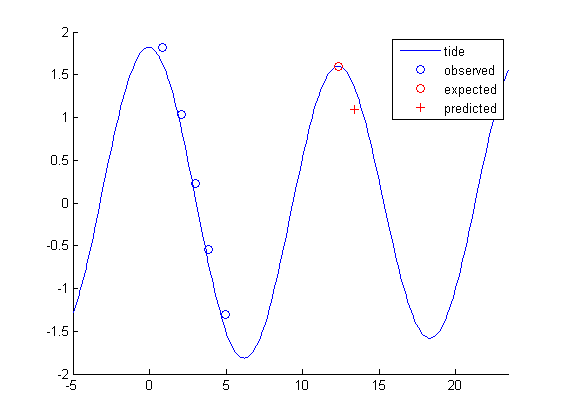
\includegraphics[width=0.6\textwidth]{edge_lin_1.png}
		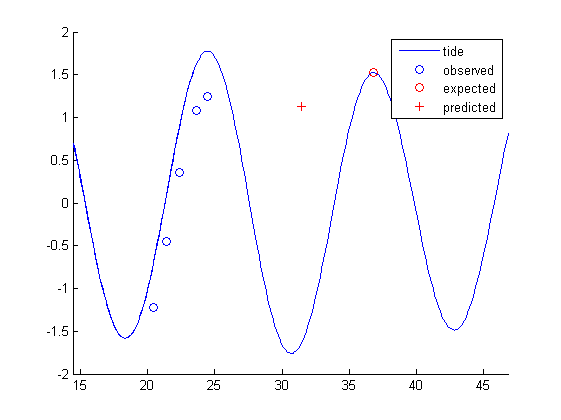
\includegraphics[width=0.6\textwidth]{edge_lin_2.png}
		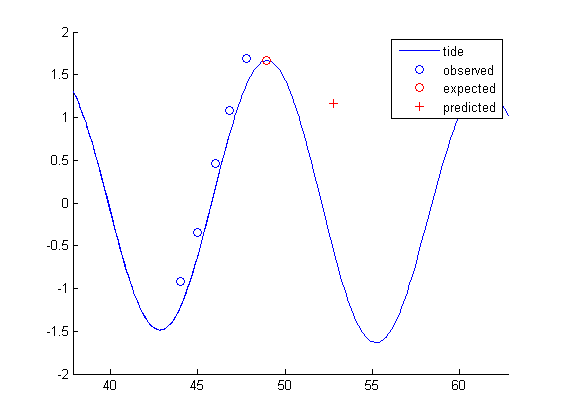
\includegraphics[width=0.6\textwidth]{edge_lin_3.png}
		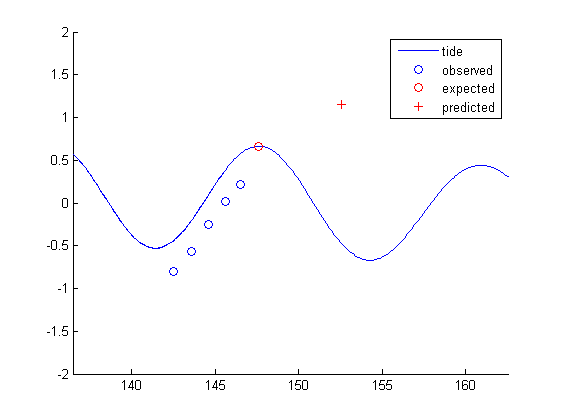
\includegraphics[width=0.6\textwidth]{edge_lin_4.png}
		\FloatBarrier
		
	\section{Predizione con Multilayer Perceptron}
		Il seguente tentativo è stato con una rete Feed-Forward, in particolare un Multilayer Perceptron.\\
		\\
		Si è subito notato come questo tipo di rete risponda molto meglio alla predizione del prossimo picco di marea rispetto alla rete lineare di Widrow, quindi si è cercato di trovare il \underline{minimo numero di neuroni} dello strato nascosto affinché l'errore medio totale potesse scendere sotto un valore accettabile, che ci è sembrato opportuno fissare al \textbf{12\%}.\\
		Il risultato è stato che \textbf{6 neuroni} rappresentano il minimo per avere un errore minore uguale a \textbf{1.02}, che corrisponde appunto al \textbf{12\%} su 8.5. Ovviamente, più neuroni fanno scendere ulteriormente l'errore, ma la crescita è molto lenta rispetto al numero di neuroni necessari, quindi il 12\% di errore con 6 neuroni sembra essere un buon compromesso.\\
		\\
		Per riprodurre tale simulazione si veda il Codice \ref{lst:tideFFEdge}.\\
		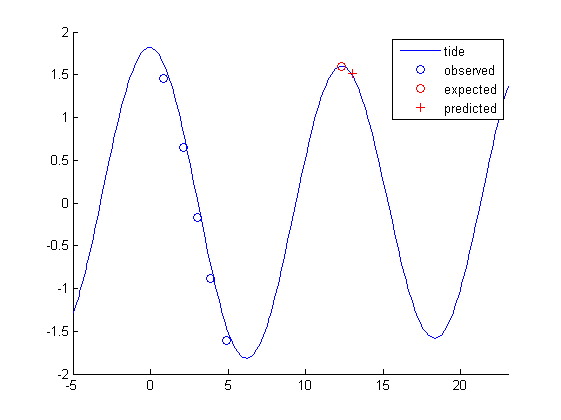
\includegraphics[width=0.6\textwidth]{edge_ff_1.png}
		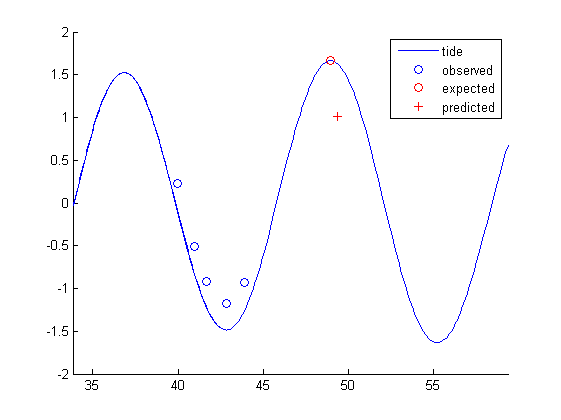
\includegraphics[width=0.6\textwidth]{edge_ff_2.png}
		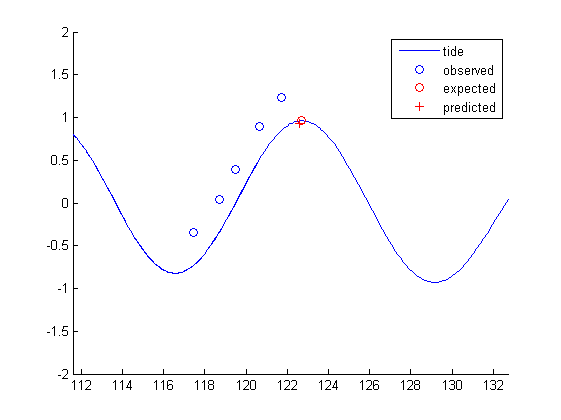
\includegraphics[width=0.6\textwidth]{edge_ff_3.png}
		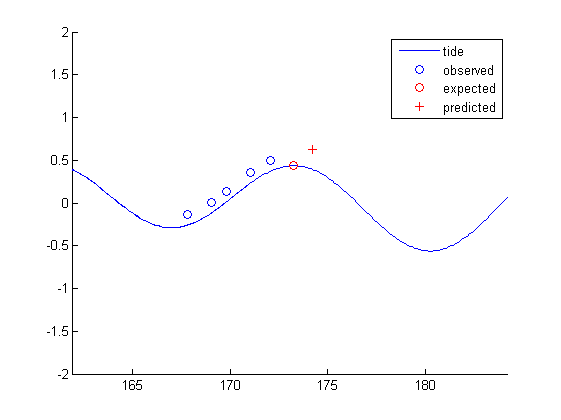
\includegraphics[width=0.6\textwidth]{edge_ff_4.png}
		\FloatBarrier
	\chapter{Calcolo del \textit{Google pagerank}}
	\label{chapterGooglePagerank}
	\minitoc \mtcskip
	\lettrine{L}{}a tecnica di ordinamento di Google si basa su l'ordinamento per importanza, detto \textbf{Google pagerank}. L'idea di base � che ``una pagina � importante se viene citata da molte pagine importanti''. Per determinare quindi l'importanza di una pagina viene implementato il cosiddetto \textbf{random surfer}, ovvero viene modellizzato un ipotetico utente che naviga sul web cliccando a caso sui link che gli si presentano davanti.\\
	Se pensiamo adesso al web come un enorme grafo orientato $W\langle V,E\rangle$, dove $V$� l'insieme dei nodi, ovvero le \textit{pagine web}, con $|V|=n$, mentre $E$ � l'insieme degli archi, ovvero i \textit{link} che collegano tra loro le pagine, allora l'importanza $x_i$ della pagina $i$-esima viene definita come
	\begin{equation}
		\label{importanzaPaginaJ}
		x_i=\sum_{(j\to i)\in E}\frac{x_j}{f_i},\qquad i=1,\dots,n,
	\end{equation}
	dove $(j\to i)$ indica il link uscente dalla pagina $j$ ed entrante nella pagina $i$, mentre $f_j$ denota il numero totale di link uscenti dalla pagina $j$. Quindi l'importanza di una pagina viene ridistribuita equamente tra le pagine in essa citate.\\
	Pi� formalmente, definendo la matrice
	\[
		L=(l_{ij})\in\mathbb{R}^{n\times n},\qquad l_{ij}=
		\begin{cases}
			1, &\text{se $(j\to i)\in E$,}\\
			0, &\text{altrimenti},
		\end{cases}
	\]
	abbiamo che
	$$f_j=\sum_{i=1}^nl_{ij},\qquad j=1,\dots,n.$$
	Definendo allora la matrice
	$$H=LF,$$
	con
	\[
		F=\begin{pmatrix}
			f_1^+ & &\\
			& \ddots &\\
			& & f_n^+
		\end{pmatrix},
		\qquad f_i^+=\begin{cases}
			\frac{1}{f_i}, &\text{se $f_i>0$},\\
			0, &\text{se $f_i=0$},
		\end{cases}
	\]
	(ovvero, $h_{ij}=\frac{l_{ij}}{f_j}$, oppure $0$ se $f_j=0$), possiamo definire il vettore del \textit{pagerank}
	\[
		\underline{\hat{x}}=\begin{pmatrix}
			x_1\\
			\vdots\\
			x_n
		\end{pmatrix},
	\]
	e riformulare la (\ref{importanzaPaginaJ}) come segue:
	\begin{equation}
		\label{calcoloImportanzaSemplice}
		\underline{\hat{x}}=H\underline{\hat{x}},
	\end{equation}
	ovvero $\underline{\hat{x}}$ � l'\textit{autovettore destro} di $H$ relativo all'autovalore $1$.\\
	Si osservi che $H$ � una matrice sparsa (cio� con molti elementi nulli) e quindi pu� essere convenientemente memorizzata in formato compresso per colonne.\\
	Il modello (\ref{calcoloImportanzaSemplice}) � tuttavia incompleto, in quanto se il \textit{random surfer} si trova in una pagina senza link in uscita non potrebbe pi� uscirne. Si ipotizza allora che quando il \textit{random surfer} si incontra in una pagina senza link uscenti, questo salta casualmente ad una pagina qualsiasi del web. Definiamo a tal proposito i vettori
	\begin{equation}
		\label{vDelta}
		\underline{v}=\begin{pmatrix}
			\frac{1}{n}\\
			\vdots\\
			\frac{1}{n}
		\end{pmatrix},
		\qquad\underline{v}=\frac{1}{n}\underline{e},\qquad \underline{\delta}=\begin{pmatrix}
			\delta_1\\
			\vdots\\
			\delta_n
		\end{pmatrix},
		\quad \delta_i=1-f_if_i^+=\begin{cases}
			1, &\text{se $f_i=0$,}\\
			0, &\text{se $f_i>0$.}
		\end{cases}
	\end{equation}
	e la matrice
	\begin{equation}
		\label{S}
		S\equiv H+\underline{v}\;\underline{\delta}^T.
	\end{equation}
	Allora la modifica appena esposta si traduce, algebricamente, nel seguente modello per il \textit{pagerank}:
	\begin{equation}
		\label{randomSurferNoLink}
		\underline{\hat{x}}=S\underline{\hat{x}}.
	\end{equation}
	\begin{teo}
		La matrice $S$ definita nella (\ref{S}) soddisfa le seguenti propriet� (le disuguaglianze sono elemento per elemento):
		\begin{enumerate}
			\item $S\geq 0$;
			\item $\underline{e}^TS=\underline{e}^T$, dove
				\[
					\underline{e}=\begin{pmatrix}
						1\\
						\vdots\\
						1
					\end{pmatrix};
				\]
			\item $\lambda=1$ � il \textit{raggio spettrale} di $S$ (dove con raggio spettrale, indicato dal simbolo $\rho(S)$, si intende il massimo autovalore, in valore assoluto di una matrice).
		\end{enumerate}
	\end{teo}
	Tuttavia, affinch� il \textit{pagerank} abbia significato fisico, vogliamo che sia a componenti strettamente positive ed unico, utilizzando la normalizzazione:
	\begin{equation}
		\label{normaXHat}
		||\underline{\hat{x}}||_1=\underline{e}^T\underline{\hat{x}}=1.
	\end{equation}
	\begin{teo}[Perron-Frobenius]
		\label{teoPerronFrobenius}
		Sia $A>0$, allora:
		\begin{enumerate}
			\item esiste $\lambda>0$, $\lambda\in\sigma(A)$ (dove $\sigma(A)$ indica lo spettro di $A$, ovvero l'insieme dei suoi autovalori), tale che $\lambda=\rho(A)$. inoltre, $\lambda$ � un \textit{autovalore semplice} (ovvero se � una radice semplice del polinomio caratteristico $p(\lambda)=det(A-\lambda I)$) e separa in modulo ogni altro autovalore di $A$;
			\item ad esso corrisponde un autovettore a componenti positive.
		\end{enumerate}
	\end{teo}
	\begin{teo}[Perron-Frobenius (forma debole)]
		Sia $A\geq 0$, allora:
		\begin{enumerate}
			\item esiste $\lambda\geq 0$, $\lambda\in\sigma(A)$, tale che $\lambda=\rho(A)$;
			\item ad esso corrisponde un autovettore a componenti non negative.
		\end{enumerate}
	\end{teo}
	Perci�, per il Teorema \ref{teoPerronFrobenius}, se avessimo $S>0$, avremo sicuramente l'autovettore del \textit{pagerank} unico e a componenti positive.\\
	Modifichiamo quindi ulteriormente la formulazione del \textit{pagerank}, introducendo una probabilit� $p\in(0,1)$, come segue:
	\begin{equation}
		\label{pagerankProbabilit�}
		\underline{\hat{x}}=S(p)\underline{\hat{x}}\equiv (pS+(1-p)\underline{v}\;\underline{e}^T)\underline{\hat{x}}.
	\end{equation}
	Questo equivale a dire che, con probabilit� $p$ il \textit{random surfer} si comporter� esattamente come descritto nella (\ref{randomSurferNoLink}), mentre con probabilit� $(1-p)$ salter� casualmente ad una qualsiasi pagina del web.\\
	Si pu� vedere che la matrice $S(p)$ verifica le ipotesi del Teorema \ref{teoPerronFrobenius}, ovvero $S(p)>0$, quindi esiste il vettore del \textit{pagerank} a componenti positive e il calcolo di tale vettore di riduce al calcolo dell'autovettore della matrice $S(p)$ relativo all'autovalore $\lambda=1$. Inoltre si ha che
	\begin{equation}
		\label{normaS(p)}
		||S(p)||_1=||\underline{e}^TS(p)||_{\infty}=1,\qquad p\in(0,1).
	\end{equation}
	
	\section{Il metodo delle potenze}
		Studiamo adesso il metodo delle potenze, grazie al quale potremo calcolare l'\textit{autovalore dominante} (\textit{semplice}) ed il corrispondente \textit{autovettore} di una data matrice. Ovvero calcolare, data $A\in\mathbb{R}^{n\times n}$, $\lambda_1$ e $\underline{v_1}\neq 0$, tali che
		\begin{equation}
			\label{equazioneAutovettAutoval}
			A\underline{v_1}=\lambda_1\underline{v_1},
		\end{equation}
		con
		$$|\lambda_1|=\rho(A)>|\lambda_2|\geq\dots\geq|\lambda_n|,\qquad\{\lambda_i\}=\sigma(A).$$
		Supponiamo, per semplicit�, che gli autovalori siano tutti \textit{distinti} e \textit{reali}:
		$$\lambda_i\neq\lambda_j,\qquad i\neq j,\qquad \lambda_i\in\mathbb{R},\qquad i=1,\dots,n,$$
		in questo modo anche gli autovettori corrispondenti saranno a componenti reali:
		$$0\neq\underline{v_i}\in\mathbb{R}^n,\qquad i=1,\dots,n.$$
		Possiamo riscrivere l'equazione (\ref{equazioneAutovettAutoval}) in forma matriciale come segue:
		\begin{align*}
			AV&=V\Lambda,\\
			V=(\underline{v_1},\dots,\underline{v_n}),&\qquad\Lambda=\begin{pmatrix}
					\lambda_1 & &\\
					& \ddots &\\
					& & \lambda_n
				\end{pmatrix},
		\end{align*}
		ovvero con $V$ matrice che presenta gli autovettori lungo le sue colonne e $\Lambda$ matrice con gli autovettori corrispondenti sulla sua diagonale principale.
		\begin{teo}
			Se gli autovalori di una matrice sono distinti, allora i corrispondenti autovettori sono \textit{linearmente indipendenti}.
		\end{teo}
		Essendo, per il teorema appena enunciato, gli autovettori di $A$ linearmente indipendenti, essi possono costituire una base per $\mathbb{R}^n$. Consideriamo quindi un vettore casuale costruito su tale base:
		\[
			\underline{x_0}=V\alpha=(\underline{v_1},\dots,\underline{v_n})\begin{pmatrix}
				\alpha_1\\
				\vdots\\
				\alpha_n
			\end{pmatrix}=
			\sum_{i=1}^n\alpha_i\underline{v_i},\qquad\alpha_i\in\mathbb{R},
		\]
		e costruiamo la successione
		$\underline{x_k}=A\underline{x_{k-1}}=\dots=A^k\underline{x_0}=A^kV\alpha.$
		Per la (\ref{equazioneAutovettAutoval})
		\begin{align*}
			\underline{x_k}&=A^kV\alpha=A^{k-1}(AV)\alpha=A^{k-1}V\Lambda\alpha=\dots=V\Lambda^k\alpha=\sum_{i=1}^n\underline{v_i}\lambda_i^k\alpha_i\\
			&=\underline{v_1}\lambda_1^k\alpha_1+\sum_{i=2}^n\underline{v_i}\lambda_i^k\alpha_i=\lambda_1^k\left(\alpha_1\underline{v_1}+\sum_{i=2}^n \left(\frac{\lambda_i}{\lambda_1}\right)^k\alpha_i\underline{v_i}\right).
		\end{align*}
		Dato che, per il Teorema \ref{teoPerronFrobenius}, $\lambda_1$ separa in modulo tutti gli altri autovalori, si ricava che
		$$\left(\frac{\lambda_i}{\lambda_1}\right)^k\rightarrow 0,\qquad k\rightarrow\infty,\qquad i=2,\dots,n.$$
		Quindi si pu� stimare che
		$$\underline{x_k}=\lambda_1^k\left(\alpha_1\underline{v_1}+\sum_{i=2}^n \left(\frac{\lambda_i}{\lambda_1}\right)^k\alpha_i\underline{v_i}\right)\approx \lambda_1^k\alpha_1\underline{v_1},\qquad k\gg 1.$$
		Se proviamo a moltiplicare il vettore $k$-esimo della successione con il $(k+1)$-esimo, otteniamo:
		$$\underline{x_k}^T\underline{x_{k+1}}\approx(\lambda_1^k\alpha_1\underline{v_1})^T(\lambda_1^{k+1}\alpha_1\underline{v_1})=\lambda_1(\lambda_1^k\alpha_1\underline{v_1})^T(\lambda_1^k\alpha_1\underline{v_1})=\lambda_1\underline{x_k}^T\underline{x_k}=\lambda_1||\underline{x_k}||_2^2,$$
		dalla quale si ricava, infine, un'approssimazione per l'autovalore dominante:
		$$\lambda_1\approx\frac{\underline{x_k}^T\underline{x_{k+1}}}{||\underline{x_k}||_2^2},\qquad k\gg 1,$$
		prendendo $\underline{x_{k+1}}$ come approssimazione dell'autovettore dominante corrispondente.\\
		Ovviamente, in fase di implementazione, si deve porre attenzione a possibili \textit{overflow} o \textit{underflow}. Per ovviare a questo tipo di problemi, ad ogni passo del metodo delle potenze si normalizza il vettore $\underline{x_k}$.\\
		Di seguito, proponiamo un'implementazione in \textsc{Matlab} del metodo delle potenze:
		\lstinputlisting[caption={Metodo delle potenze.}]{code/metodoPotenze.m}

		\subsection{Metodo delle potenze per il \textit{Google pagerank}}
			Nel caso del calcolo del \textit{Google pagerank} sappiamo che l'autovalore corrispondente all'autovettore dominante � $\lambda=1$, quindi non ci sar� bisogno n� di calcolarlo, n� di normalizzare di volta in volta il vettore $\underline{x_k}$. Per questo motivo non si rischia di incorrere in \textit{overflow}/\textit{underflow}.\\
			Se inoltre prendiamo come vettore iniziale un vettore $\underline{x_0}$ tale che
			$$\underline{x_0}>0,\qquad \underline{e}^T\underline{x_0}=||\underline{x_0}||_1=1,$$
			per induzione (grazie alla (\ref{normaS(p)})) si ha:
			\begin{align}
				&\underline{x_k}=S(p)\underline{x_{k-1}}>0,\notag\\
				\label{normaXk}
				&||\underline{x_k}||_1=\underbrace{\underline{e}^TS(p)}_{\underline{e}^T}\underline{x_{k-1}}=\underline{e}^T\underline{x_{k-1}}=||\underline{x_{k-1}}||_1=1.
			\end{align}
			Quindi, per la (\ref{pagerankProbabilit�}), possiamo ricavare come segue un criterio d'arresto per il metodo delle potenze:
			\begin{align*}
				||\underline{x_k}-\underline{\hat{x}}||_1&= ||S(p)\underline{x_{k-1}}-S(p)\underline{\hat{x}}||_1=||S(p)(\underline{x_{k-1}}-\underline{\hat{x}})||_1 =\\
				&=||pS(\underline{x_{k-1}}-\underline{\hat{x}})+(1-p)\underline{v}\;\underbrace{\underline{e}^T(\underline{x_{k-1}}-\underline{\hat{x}})}_{=0}||_1=||pS(\underline{x_{k-1}}-\underline{\hat{x}})||_1\leq\\
				&\leq p\underbrace{||S||_1}_{=||\underline{e}^TS||_{\infty}=1}\cdot||\underline{x_{k-1}}-\underline{\hat{x}}||_1=p||\underline{x_{k-1}}-\underline{\hat{x}}||_1\leq\dots\leq\\
				&\leq p^k||\underline{x_0}-\underline{\hat{x}}||_1\leq 2p^k.
			\end{align*}
			Quindi si ricava che per avere un risultato entro la tolleranza fissata $tol$, basta fare, al pi�, $\frac{\log tol-\log 2}{\log p}$. Si osserva che valori di $p$ vicini ad $1$ riproducono un modello pi� fedele del web ma degradano la velocit� di convergenza del metodo delle potenze. Studi in proposito indicano $p=0.85$ come un buon compromesso tra \textit{accuratezza} ed \textit{efficienza}.\\
			\\
			Per quanto riguarda il \underline{costo computazionale} del metodo delle potenze, si ha che ogni iterazione si riduce al calcolo di (ricordando che $\underline{v}=\frac{1}{n}\underline{e}$):
			\begin{align}
				\underline{x_k} &= pS\underline{x_{k-1}} + (1-p)\underline{v}\;\underbrace{\underline{e}^T\underline{x_{k-1}}}_{=1}=\notag\\
				&=p(H+\underline{v}\;\underline{\delta}^T)\underline{x_{k-1}}+(1-p)\underline{v}=\notag\\
				\label{metodoPotenzeGooglepgrank}
				&=p(H\underline{x_{k-1}})+\frac{1+p(\underline{\delta}^T\underline{x_{k-1}}-1)}{n}\underline{e}.
			\end{align}
			Quest'operazione � composta da:
			\begin{itemize}
				\item un prodotto matrice-vettore, $H\underline{x_{k-1}}$, del costo di $O(n)$ \texttt{flops};
				\item un prodotto scalare, $\underline{\delta}^T\underline{x_{k-1}}$, del costo di $2n$ \texttt{flops};
				\item l'operazione complessiva, che � del tipo
					\begin{center}
						vettore = scalare*vettore + scalare*vettore,
					\end{center}
					che costa altri $3n$ \texttt{flops}.
			\end{itemize}
			Quindi il costo complessivo si vede essere \textbf{lineare} rispetto alla dimensione del problema, sia in termini di operazioni eseguite che di memoria occupata (memorizzando la matrice sparsa $H$ in formato compresso per colonne).\\
			Secondo le osservazioni appena fatte, il metodo delle potenze per il calcolo del Google \textit{pagerank} pu� essere implementato efficientemente come segue:
			\lstinputlisting[caption={Metodo delle potenze per il calcolo del Google \textit{pagerank}.}]{code/metodoPotenzeGooglePagerank.m}
	\section{Risoluzione iterativa di sistemi lineari}
		Un approccio differente al metodo delle potenze per il calcolo del \textit{Google pagerank} � la risoluzione iterativa di sistemi lineari.\\
		Si vede che, per le (\ref{vDelta}), (\ref{normaXHat}) e (\ref{pagerankProbabilit�}):
		\begin{align*}
			&\underline{\hat{x}}=S(p)\underline{\hat{x}}=pS\underline{\hat{x}}+(1-p)\frac{1}{n}\underline{e}\;\underbrace{\underline{e}^T\underline{\hat{x}}}_{=1},\\
			&\underline{\hat{x}}-pS\underline{\hat{x}}=\frac{1-p}{n}\underline{e},\\
			&\underbrace{(I-pS)}_{\equiv A}\underline{\hat{x}}=\underbrace{\frac{1-p}{n}\underline{e}}_{\equiv\underline{b}}.
		\end{align*}
		Quindi il problema (\ref{pagerankProbabilit�}) pu� essere riformulato come segue:
		\begin{equation}
			\label{sistemaPagerank}
			A\underline{\hat{x}}=\underline{b}.
		\end{equation}
		Risulta chiaro che, data la sparsit� della matrice $A$, non � conveniente utilizzare i metodi di fattorizzazione visti nel Capitolo \ref{chap:sistemiLinENonLin}.Un'importante caratteristica della matrice $A$ � quella di poter essere scritta nella forma
		\begin{equation}
			\label{A}
			A=I-B,\qquad B\geq 0,\qquad \rho(B)<1,
		\end{equation}
		infatti risulta che $B=I-I+pS=pS$ e si ha che $S\geq 0$, $\rho(S)=1$ e $p<1$.
		\begin{teo}
			\label{teoMatriceConvergente}
			Una matrice $B$ ha raggio spettrale minore di $1$, ovvero $\rho(B)<1$, se e solo se
			$$B^i\rightarrow O,\qquad i\rightarrow\infty.$$
		\end{teo}
		\begin{defi}
			Per il Teorema \ref{teoMatriceConvergente}, una matrice avente raggio spettrale minore di $1$ si dice \textbf{convergente}.
		\end{defi}
		\begin{defi}
			Una matrice del tipo $\alpha A$, con $A$ definita nella (\ref{A}) ed $\alpha>0$, si dice \textbf{M-matrice}.
		\end{defi}
		\begin{teo}
			\label{teoM-Matrice}
			Se $A$ � una M-matrice, allora $A^{-1}\geq 0$
		\end{teo}
		Le \textit{M-matrici} inoltre risultano essere \textbf{matrici monotone}, ovvero tali che
		$$A\underline{x}\leq\underline{y}\qquad\Rightarrow\qquad\underline{x}\leq A^{-1}\underline{y},$$
		o, pi� in generale, se $C$ � una matrice delle stesse dimensioni di $A$, tali che
		$$A\leq C\qquad\Rightarrow\qquad I\leq A^{-1}C,\quad I\leq CA^{-1},$$
		dove le disuguaglianze sono da intendersi elemento per elemento.
		\begin{defi}
			Si parla di \textbf{splitting} della matrice $A$ qualora si possa scrivere
			\begin{equation}
				\label{splitting}
				A=M-N,
			\end{equation}
			con $det(M)\neq 0$.
		\end{defi}
		Lo \textit{splitting} della matrice $A$ viene definito in modo tale che i sistemi lineari con la matrice $M$ come matrice dei coefficienti siano immediatamente risolvibili senza bisogno di fattorizzazione. Questo perch�, per le (\ref{sistemaPagerank}) e (\ref{splitting}), si pu� definire il seguente metodo iterativo per calcolare un'approssimazione del vettore di \textit{pagerank}:
		\begin{equation}
			\label{metodoIterativoSplitting}
			M\underline{x_k}=N\underline{x_{k-1}}+\underline{b},\qquad k\geq 1,
		\end{equation}
		partendo da un'approssimazione data $x_0$. Definiamo l'errore al passo $k$, come
		\begin{equation}
			\label{erroreSplitting}
			\underline{e_k}=\underline{x_k}-\underline{\hat{x}}.
		\end{equation}
		Osservando che $$M\underline{\hat{x}}=N\underline{\hat{x}}+\underline{b}$$ e per la (\ref{metodoIterativoSplitting}) si ottiene la seguente \textit{equazione dell'errore}:
		\begin{align*}
			\underline{e_k} &= \underline{x_k}-\underline{\hat{x}} = M^{-1}(N\underline{x_{k-1}}+\underline{b})-M^{-1}(N\underline{\hat{x}}+\underline{b})=\\
			&= M^{-1}(N\underline{x_{k-1}}+\underline{b}-N\underline{\hat{x}}-\underline{b})=\\
			&= M^{-1}N(\underline{x_{k-1}}-\underline{\hat{x}})=\\
			&= M^{-1}N\underline{e_{k-1}},\qquad k\geq 1,
		\end{align*}
		dalla quale si ricava
		$$\underline{e_k}=(M^{-1}N)^k\underline{e_0},\qquad k\geq 1.$$
		Quindi, per il Teorema \ref{teoMatriceConvergente}, il metodo sar� convergente se e solo se la matrice $M^{-1}N$ � convergente, ovvero se e solo se $\rho(M^{-1}N)<1$.
		\begin{defi}
			La matrice $M^{-1}N$ dello splitting (\ref{splitting}) si dice \textbf{matrice di iterazione} del metodo (\ref{metodoIterativoSplitting}).
		\end{defi}
		Per quanto visto nello studio del metodo delle potenze e supponendo che la matrice d'iterazione abbia un autovalore dominante semplice, si ottiene la stima
		$$||\underline{e_k}||\approx\rho(M^{-1}N)^k||\underline{e_0}||,\qquad k\gg 1.$$
		Quindi il raggio spettrale della matrice d'iterazione ci permette di confrontare tra loro metodi iterativi definiti da diversi splitting della matrice $A$.
		
		\subsection{\textit{Splitting} regolari di matrici}
			\begin{defi}
				Lo splitting (\ref{splitting}) si dice \textbf{regolare} se
				$$m^{-1}\geq 0,\qquad N\geq 0.$$
			\end{defi}
			\begin{lem}
				\label{lemmaMatriciOrdinate}
				Siano $A,B\in\mathbb{R}^{n\times n}$, $A\geq B\geq 0$. Allora $A^i\geq B^i\geq 0$, $i\geq 0$.
			\end{lem}
			\begin{lem}
				\label{lemmaMatriciOrdinate2}
				Siano $A,B\in\mathbb{R}^{n\times n}$, $A\geq B\geq 0$. Allora $\rho(A)\geq\rho(B)$.
			\end{lem}
			\begin{teo}
				Se lo splitting (\ref{splitting}) � regolare e $A^{-1}\geq 0$, allora il metodo iterativo (\ref{metodoIterativoSplitting}) � convergente
			\end{teo}
			\begin{cor}
				Se lo splitting (\ref{splitting}) � regolare ed $A$ � una M-matrice, allora il metodo iterativo (\ref{metodoIterativoSplitting}) � convergente (vedi Teorema \ref{teoM-Matrice}).
			\end{cor}
			Per i Lemmi \ref{lemmaMatriciOrdinate} e \ref{lemmaMatriciOrdinate2} si hanno i seguenti due corollari:
			\begin{cor}
				\label{corMmatrice}
				Se $A=\alpha(I-B)$ � una M-matrice e $A=M-N$, con $0\leq N\leq\alpha B$, allora M � nonsingolare e lo splitting � regolare. Pertanto, il metodo (\ref{metodoIterativoSplitting}) � convergente.
			\end{cor}
			\begin{cor}
				\label{corMmatrice2}
				Se $A$ � una M-matrice e la matrice $M$ in (\ref{splitting}) � ottenuta ponendo a $0$ gli elementi extradiagonali di $A$, allora lo splitting (\ref{splitting}) � regolare. Pertanto il metodo iterativo (\ref{metodoIterativoSplitting}) � convergente.
			\end{cor}

			Infine quest'ultimo Teorema ci consente di comparare tra loro le velocit� di due metodi iterativi costruiti su due diversi splitting regolari di una stessa matrice:
			\begin{teo}
				\label{teoVelocit�ConvergenzaSplitting}
				Siano $A=M_1-N_1=M_2-N_2$ due splitting regolati di $A$, matrice tale che $A^{-1}\geq 0$. Se $N_1\leq N_2$, allora $\rho(M^{-1}_1N_1)\leq\rho(M^{-1}_2N_2)$, ovvero il primo splitting converge pi� velocemente del secondo.
			\end{teo}
		\subsection{Criteri d'arresto}
			Per quanto riguarda i criteri d'arresto del metodo iterativo (\ref{metodoIterativoSplitting}) si pu� pensare a controllare la norma $||\underline{x_k}-\underline{x_{k-1}}||$. Un'altra possibilit�, invece, � quella di controllare la norma del \textit{vettore residuo}:
			\begin{equation}
				\label{residuoSplitting}
				\underline{r_k}=A\underline{x_k}-\underline{b}.
			\end{equation}
			Si osserva che il vettore residuo $\underline{r_k}$ ed il vettore d'errore $\underline{e_k}$ sono in stretta relazione tra loro, infatti:
			$$A\underline{e_k}=\underline{r_k}.$$
		\subsection{I metodi di Jacobi e Gauss-Seidel}
			Consideriamo il partizionamento della matrice $A$
			\begin{equation}
				\label{splittingDLU}
				A=D-L-U,
			\end{equation}
			con
			\begin{itemize}
				\item $D$ diagonale,
				\item $L$ strettamente triangolare inferiore e
				\item $U$ strettamente triangolare superiore.
			\end{itemize}
			\begin{teo}
				\label{teoDLUmaggiori0}
				Se la matrice $A$ in (\ref{splittingDLU}) � una M-matrice, allora $D,L,U\geq 0$. In particolare $D$ ha elementi diagonali positivi ($D>0$).
			\end{teo}

			\begin{teo}
				Se $A$ in (\ref{splittingDLU}) � una M-matrice, allora tali sono anche le matrici $D$ e $D-L$.
			\end{teo}
			\begin{defi}$\;$\\
				\begin{itemize}
					\item Lo splitting
						$$A=M_J-N_J\equiv D-(L+U)$$
						definisce il metodo iterativo di \textbf{Jacobi}.
					\item Lo splitting
						$$A=M_{GS}-N_{GS}\equiv (D-L)-U$$
						definisce il metodo iterativo di \textbf{Gauss-Seidel}
				\end{itemize}
			\end{defi}
			\begin{cor}
				Se $A$ in (\ref{splittingDLU}) � una M-matrice, allora gli splitting di Jacobi e di Gauss-Seidel sono regolari e quindi i relativi metodi iterativi sono convergenti.
			\end{cor}
			Si osserva che ad ogni iterazione il metodo di Jacobi richiede la risoluzione di un sistema diagonale, mentre il metodo di Gauss-Seidel richiede la risoluzione di un sistema triangolare inferiore.
			\begin{cor}
				Se $A$ in (\ref{splittingDLU}) � una M-matrice, allora
				$$\rho((D-L)^{-1}U)\leq\rho(D^{-1}(L+U))<1.$$
				Ovvero, in generale, il metodo di Gauss-Seidel converge pi� velocemente del metodo di Jacobi.
			\end{cor}
			Infatti, essendo $L\geq 0$ per il Teorema \ref{teoDLUmaggiori0}, sicuramente $U\leq(L+U)$ (vedi Teorema \ref{teoVelocit�ConvergenzaSplitting}).\\
			\\
			Concludendo, osserviamo che, per quanto detto fin'ora sugli splitting regolari di matrici, i metodi iterativi di Jacobi e di Gauss-Seidel (ed in particolare quest'ultimo) possono essere convenientemente utilizzati per calcolare un'approssimazione del vettore di \textit{pagerank} di Google.\\
			\\
			Si mostrano di seguito le implementazioni in \textsc{Matlab} dei metodi di Jacobi e di Gauss-Seidel;
			\lstinputlisting[caption={Metodo di Jacobi.}]{code/jacobi.m}
			\lstinputlisting[caption={Metodo di Gauss-Seidel.}]{code/gaussSeidel.m}

	\section*{Esercizi}
		\addcontentsline{toc}{section}{Esercizi}
		\markboth{\textsc{\uppercase{Capitolo }\ref{chapterGooglePagerank}\uppercase{. Calcolo del \textit{Google pagerank}}}}{\textsc{\uppercase{Esercizi}}}
		\begin{es}[Teorema di Gershgorin] %6.1
			Dimostrare che gli autovalori di una matrice $A=(a_{ij})\in\mathbb{C}^{n\times n}$ sono contenuti nell'insieme
			\[
				\mathcal{D}=\bigcup_{i=1}^n\mathcal{D}_i,\qquad \mathcal{D}_i=\left\{\lambda\in\mathbb{C}:|\lambda-a_{ii}|\leq\sum_{\begin{subarray}{c}
					j=1\\
					j\neq i
				\end{subarray}}^n|a_{ij}|\right\},\quad i=1,\dots,n.
			\]
		\end{es}
		\begin{sol}
			\normalfont Sia $\lambda\in\sigma{A}$ ed $\underline{x}$ il corrispondente autovettore ($\underline{x}\neq\underline{0}$ e $A\underline{x}=\lambda\underline{x}$) quindi $\underline{e}_i^TA\underline{x}=\lambda\underline{e}_i^T\underline{x}$ per $i=1,\ldots,n$ cio� $\sum_{j=1}^n{a_{i,j}x_j}=\lambda x_i$; posto $i$ tale che $|x_i|\geq|x_j|$ ($x_i\neq 0$) risulta $\lambda=\frac{\sum_{j=1}^n{a_{i,j}x_j}}{x_i}=a_{i,i}+\sum_{j=1\: j\neq i}^n{a_{i,j}\frac{x_j}{x_i}}$ ovvero $\lambda-a_{i,i}=\sum_{j=1\: j\neq i}^n{a_{i,j}\frac{x_j}{x_i}}$. Passando ai valori assoluti $$\left|\lambda-a_{i,i}\right|=\left|\sum_{j=1\: j\neq i}^n{a_{i,j}\frac{x_j}{x_i}}\right|\leq\sum_{j=1\: j\neq i}^n{\left|a_{i,j}\frac{x_j}{x_i}\right|}\leq\sum_{j=1\: j\neq i}^n{\left|a_{i,j}\right|}$$ poich� $\left|\frac{x_j}{x_i}\right|\leq 1$ in quanto $|x_i|\geq|x_j|$. Segue $\lambda\in\bigcup_{i=1}^{n}{\mathcal{D}_i}$ da cui $\sigma{A}\subseteq\mathcal{D}$.
		\end{sol}
		\sectionline
		\begin{es} %6.2
			\label{es:6.2}
			Utilizzare il metodo delle potenze per approssimare l'autovalore dominante della matrice
			\[
				A_n=\begin{pmatrix}
					2 & -1 & &\\
					-1 & 2 & \ddots &\\
					& \ddots & \ddots & -1\\
					& & -1 & 2
				\end{pmatrix}\in\mathbb{R}^{n\times n},
			\]
			per valori crescenti di $n$. Verificare numericamente che questo � dato da $2\left(1+\cos\frac{\pi}{n+1}\right)$.
		\end{es}
		\begin{sol}
			\normalfont 
			Prima di applicare il metodo delle potenze, mostriamo che $A_n$ pu� essere scritta come una M-matrice, infatti: $A_n=2(I_n-B_n)$ dove $$B_n=\begin{pmatrix}0&1/2&&\\1/2&0&\ddots&\\&\ddots&\ddots&1/2\\&&1/2&0\end{pmatrix}\in\mathbb{R}^{n\times n}.$$ Risulta $\lambda_j(B_n)=\cos{\frac{j\pi}{n+1}}$, $|\lambda_j|\leq 1$, per $j=1,\ldots,n$; segue $\lambda_j(A_n)=2(\lambda_j(I_n)-\lambda_j(B_n))=2(1-\cos{\frac{j\pi}{n+1}})$; il massimo � $\lambda=2(1+\cos{\frac{\pi}{n+1}})$.
			La verifica numerica di questo risultato � riportata nelle seguenti tabelle.
			\begin{center}\begin{tabular}{c|c|c|c}
			\hline\multicolumn{4}{c}{Tolleranza $tol=10^{-5}$}\\\hline
			$n$ & $\lambda_1$ & $2\left(1+\cos{\frac{\pi}{n+1}}\right)$ & scostamento\\\hline
			10 & 3.9189 & 3.9190 & 0.0001 \\
			15 & 3.9614 & 3.9616 & 0.0002 \\
			20 & 3.9774 & 3.9777 & 0.0003 \\
			25 & 3.9853 & 3.9854 & 0.0002 \\
			30 & 3.9891 & 3.9897 & 0.0006 \\
			35 & 3.9921 & 3.9924 & 0.0003 \\
			40 & 3.9929 & 3.9941 & 0.0012 \\
			45 & 3.9938 & 3.9953 & 0.0015 \\
			50 & 3.9947 & 3.9962 & 0.0015 
			\end{tabular}\end{center}
			
			\begin{center}\begin{tabular}{c|c|c|c}
			\hline\multicolumn{4}{c}{Tolleranza $tol=10^{-7}$}\\\hline
			$n$ & $\lambda_1$ & $2\left(1+\cos{\frac{\pi}{n+1}}\right)$ & scostamento\\\hline
			5 & 3.7321 & 3.7321 & 0.0000 \\
			10 & 3.9190 & 3.9190 & 0.0000 \\
			15 & 3.9616 & 3.9616 & 0.0000 \\
			20 & 3.9777 & 3.9777 & 0.0000 \\
			25 & 3.9854 & 3.9854 & 0.0000 \\
			30 & 3.9897 & 3.9897 & 0.0000 \\
			35 & 3.9924 & 3.9924 & 0.0000 \\
			40 & 3.9941 & 3.9941 & 0.0000 \\
			45 & 3.9953 & 3.9953 & 0.0000 \\
			50 & 3.9962 & 3.9962 & 0.0000  
			\end{tabular}\end{center}
			\begin{flushright}
				\underline{Riferimenti \textsc{Matlab}}\\
				Codice \ref{lst:es6.2} (pagina \pageref{lst:es6.2})
			\end{flushright}
		\end{sol}
		\sectionline
		\begin{es} %6.3
			Dimostrare i Corollari \ref{corMmatrice} e \ref{corMmatrice2}.
		\end{es}
		\begin{sol}
			\normalfont
			\underline{Corollario 6.2}\\
			Sia $A=\alpha(I-B)=M-N$ con $0\leq N\leq\alpha B$ quindi $M=\alpha I-\alpha B+N=\alpha I-\alpha B+\alpha Q=\alpha(I-(B-Q))$ con $\alpha Q=N\leq\alpha B$ e $0\leq Q\leq B$. Dato che $0\leq B-Q\leq B$, per il Lemma 6.2, $\rho(B-Q)\leq\rho(B)\leq 1$. Quindi $M$ � una M-matrice; lo splitting � regolare infatti $M^{-1}\geq 0$ ($M$ � una M-matrice) e $B-Q\geq 0$.\\
			\\\underline{Corollario 6.3}\\
			Sia $A=M-N$ M-matrice con $M=diag(A)$ allora la matrice $A-M=B$ avr� elementi nulli sulla diagonale e, altrove, gli elementi di $A$. Poich� $A=\alpha(I-B)=\alpha I-\alpha B=M-N$, risulta $\alpha B=N$ quindi, per il Corollario 6.2, lo splitting � regolare ed il metodo � convergente.
		\end{sol}
		\sectionline
		\begin{es} %6.4
			Dimostrare il Teorema \ref{teoDLUmaggiori0}.
		\end{es}
		\begin{sol}
			\normalfont
			Poich� $A$ � una M-matrice, essa pu� essere scritta nella forma $A=\alpha(I-B)$ con $B\geq 0$ e $\rho(B)<1$; inoltre, per ipotesi, $A=D-L-U$ da cui si deduce che $D=\alpha(I-diag(B))$ e $(L+U)=\alpha(B-diag(B))$.\\
			La matrice $(L+U)=\alpha(B-diag(B))$ risulta maggiore di zero in quanto $B>0\rightarrow (B-diag(B))>0$.
			La matrice $D$ ha elementi positivi sulla diagonale: supponiamo per assurdo $a_{i,i}\leq 0$: l'$i$-esima riga di $A$, negativa, � data da $A\underline{e}_i\leq\underline{0}$ dato che $A$ � una M-matrice risulta $\underline{e}_i\leq A^{-1}\underline{0}=\underline{0}$ assurdo poich� $\underline{e}_i\geq\underline{0}, \forall i$.
		\end{sol}
		\sectionline
		\begin{es} %6.5
			Tenendo conto della (\ref{normaXk}), riformulare il metodo delle potenze (\ref{metodoPotenzeGooglepgrank}) per il calcolo del \textit{Google pagerank} come metodo iterativo definito da uno splitting regolare.
		\end{es}
		\begin{sol}
			\normalfont
			Il problema del \textsl{Google pagerank} � $S(p)\hat{\underline{x}}=\hat{\underline{x}}$ dove $S(p)=pS+(1-p)\underline{v}\:\underline{e}^{T}$. Sostituendo, risulta $$(pS+(1-p)\underline{v}\:\underline{e}^{T})\hat{\underline{x}}=\hat{\underline{x}}\quad\Rightarrow\quad (I-pS)\hat{\underline{x}}=(1-p)\underline{v}\:\underline{e}^T\hat{\underline{x}}$$
			Dato che $\underline{v}=\frac{1}{n}\underline{e}$ ed $e^T\hat{\underline{x}}=1$ si ricava
			$$(I-pS)\hat{\underline{x}}=\frac{1-p}{n}\underline{e}.$$
			Si pu� infine definire il seguente metodo iterativo:
			$$I\underline{x}_{k+1}=pS\underline{x}_k+\dfrac{1-p}{n}\underline{e}.$$
			Il metodo � convergente in quanto la matrice di iterazione ha raggio spettrale minore di $1$: $\rho(I^{-1}pS)=\rho(pS)<1$ dato che $p \in (0,1)$ e $\rho(S)=1$.
		\end{sol}
		\sectionline
		\begin{es} %6.6
			Dimostrare che il metodo di Jacobi converge asintoticamente in un numero minore di iterazioni, rispetto al metodo delle potenze (\ref{metodoPotenzeGooglepgrank}) per il calcolo del \textit{Google pagerank}.
		\end{es}
		\begin{sol}
			\normalfont 
			La matrice di iterazione di Jacobi ha raggio spettrale minore di 1 mentre, nel calcolo del \textsl{Google pagerank}, l'autovalore dominante � $\lambda=1$ quindi il raggio spettrale di tale matrice � esattamente 1. Poich� il raggio spettrale della matrice di iterazione del metodo di Jacobi � minore del raggio spettrale della matrice del \textsl{Google pagerank}, il metodo di Jacobi converge in asintoticamente in un numero minore di iterazioni, rispetto al metodo delle potenze per il calcolo del \textsl{Google pagerank}.
		\end{sol}
		\sectionline
		\begin{es} %6.7
			Dimostrare che, se $A$ � diagonale dominante, per riga o per colonna, il metodo di Jacobi � convergente.
		\end{es}
		\begin{sol}
			\normalfont 
			Nel metodo di Jacobi si ha $A=M-N=D-(L+U)$ quindi $$M=\begin{pmatrix}a_{1,1}&&&\\&\ddots&&\\&&\ddots&\\&&&a_{n,n}\end{pmatrix}\mbox{ e } N=\begin{pmatrix}0&a_{1,2}&\ldots&a_{1,n}\\a_{2,1}&\ddots&\ddots&\vdots\\\vdots&\ddots&\ddots&a_{n-1,n}\\a_{n,1}&\ldots&a_{n,n-1}&0\end{pmatrix}.$$ Si ha $$B=M^{-1}N=\begin{pmatrix}\frac{1}{a_{1,1}}&&&\\&\ddots&&\\&&\ddots&\\&&&\frac{1}{a_{n,n}}\end{pmatrix}\begin{pmatrix}0&a_{1,2}&\ldots&a_{1,n}\\a_{2,1}&\ddots&\ddots&\vdots\\\vdots&\ddots&\ddots&a_{n-1,n}\\a_{n,1}&\ldots&a_{n,n-1}&0\end{pmatrix}=$$$$=\begin{pmatrix}0&\frac{a_{1,2}}{a_{1,1}}&\ldots&\frac{a_{1,n}}{a_{1,1}}\\\frac{a_{2,1}}{a_{2,2}}&\ddots&\ddots&\vdots\\\vdots&\ddots&\ddots&\frac{a_{n-1,n}}{a_{n-1,n-1}}\\\frac{a_{n,1}}{a_{n,n}}&\ldots&\frac{a_{n,n-1}}{a_{n,n}}&0\end{pmatrix},$$ per il Teorema di Gershgorin risulta $$\mathcal{D}_i=\left\{\lambda\in\mathbb{C}\::\:|\lambda-b_{i,i}|\leq\sum_{j=1\: j\neq i}^{n}{|b_{i,j}|}\right\}=\left\{\lambda\in\mathbb{C}\::\:|\lambda|\leq\sum_{j=1\: j\neq i}^{n}{\left|\frac{a_{i,j}}{a_{i,i}}\right|}\right\};$$ supposta $A$ a diagonale dominante per righe, $|a_{i,i}|\geq\sum_{j=1,\: j\neq i}^n{|a_{i,j}|}$, risulta $|\lambda|\leq\frac{1}{|a_{i,i}|}\sum_{j=1\: j\neq i}^{n}{a_{i,j}}<1$. Ogni $\mathcal{D}_i$ � centrato in $0$ e ha raggio minore di $1$ quindi $\mathcal{D}=\bigcup_{i=1}^{n}{\mathcal{D}_i}$ � centrato in $0$ e ha raggio pari al raggio massimo dei $\mathcal{D}_i$ ma sempre minore di $1$. Dato che $\lambda(A)=\lambda(A^T)$, il risultato vale anche se $A$ � a diagonale dominante per colonne; il metodo di Jacobi � dunque convergente per matrici a diagonale dominante.
		\end{sol}
		\sectionline
		\begin{es} %6.8
			Dimostrare che, se $A$ � diagonale dominante, per riga o per colonna, il metodo di Gauss-Seidel � convergente.
		\end{es}
		\begin{sol}
			\normalfont 
			Nel metodo di Gauss-Seidel si ha $A=M-N=(D-L)-U$; sia $\lambda\in\sigma(M^-1N)$ quindi $\lambda$ � tale che $\det{(M^{-1}N-\lambda I)}=\det{(M^{-1}(N-\lambda M))}=\det{(M^{-1})}\det{(N-\lambda M)}=0$. Dato che, per definizione di splitting, $\det{(M^{-1})}\neq 0$ deve risultare $\det{(N-\lambda M)}=0=\det{(\lambda M-N)}$; sia $H=\lambda M-N$ matrice singolare e supponiamo, per assurdo, $|\lambda|\geq 1$. Risulta $$H=\begin{cases}\lambda a_{i,j}&\mbox{se }i\geq j,\\a_{i,j}&\mbox{altrimenti},\end{cases};$$ quindi $H$ � a diagonale dominante ma $$\sum_{j=1\: j\neq i}^n{|h_{i,j}|}\leq |\lambda|\sum_{j=1\: j\neq i}^n{|a_{i,j}|}<|\lambda||a_{i,i}|=|h_{i,i}|.$$Si ha una contraddizione poich� le matrici a diagonale dominanti sono non signolari, dunque $|\lambda|<1$ e quindi il metodo di Gauss-Seidel � convergente per matrici a diagonale dominante.
		\end{sol}
		\sectionline
		\begin{es} %6.9
			Se $A$ � \textit{sdp}, il metodo di Gauss-Seidel risulta essere convergente. Dimostrare questo risultato nel caso (assai pi� semplice) in cui l'autovalore di massimo modulo della matrice di iterazione sia reale.\\
			(\underline{Suggerimento:} considerare il sistema lineare equivalente
			$$(D^{-\frac{1}{2}}AD^{-\frac{1}{2}})(D^{\frac{1}{2}}\underline{x})=(D^{-\frac{1}{2}}\underline{b}),\qquad D^{\frac{1}{2}}=diag(\sqrt{a_{11}},\dots,\sqrt{a_{nn}}),$$
			la cui matrice dei coefficienti � ancora \textit{sdp} ma ha diagonale unitaria, ovvero del tipo $I-L-L^T$. Osservare quindi che, per ogni vettore reale $\underline{v}$ di norma $1$, si ha: $\underline{v}^TL\underline{v}=\underline{v}^TL^T\underline{v}=\frac{1}{2}\underline{v}^T(L+L^T)\underline{v}<\frac{1}{2}$.)
		\end{es}
		\begin{sol}
			\normalfont 
			Scriviamo il sistema $A\underline{x}=\underline{b}$ nella forma equivalente $$\left(D^{-1/2}AD^{-1/2}\right)\left(D^{1/2}\underline{x}\right)=\left(D^{-1/2}\underline{b}\right)$$ con $D=diag(\sqrt{a_{1,1}},\ldots,\sqrt{a_{n,n}})$. La matrice $C=\left(D^{-1/2}AD^{-1/2}\right)$ ha diagonale unitaria: $$c_{i,i}=d_i^{-1}a_{i,i}d_i^{-1}=\frac{1}{\sqrt{a_{i,i}}}a_{i,i}\frac{1}{\sqrt{a_{i,i}}}=a_{i,i};$$ inoltre � ancora sdp e scrivibile come $C=I-L-L^T$.\\
			Poich� $C$ � sdp risulta $\underline{v}^TA\underline{v}>0, \forall\underline{v}\neq\underline{0}$ cio� $$\underline{v}^T\underline{v}>\underline{v}^TL\underline{v}+\underline{v}^TL^T\underline{v}\quad\Rightarrow\quad\underline{v}^TL\underline{v}=\underline{v}^TL^T\underline{v}<\frac{1}{2}.$$
			Sia $|\lambda|=\rho(M_{GS}^{-1}N_{GS})=\rho\left((I-L)^{-1}L^T\right)$ assunto reale e $\underline{v}$ il corrispondente autovettore, dunque $$(I-L)^{-1}L^T=\lambda\underline{v}\quad\Rightarrow\quad\lambda\underline{v}=L^T\underline{v}+\lambda L\underline{v}$$ ovvero $\lambda=\underline{v}^TL\underline{v}+\lambda\underline{v}^TL\underline{v}=(1+\lambda)\underline{v}^TL)\underline{v}$ da cui $$\frac{\lambda}{1+\lambda}=\underline{v}^TL\underline{v}<\frac{1}{2}\quad\Rightarrow\quad -1<\lambda<1.$$
			Segue $\rho(M_{GS}^{-1}N_{GS})=|\lambda|<1$.
		\end{sol}
		\sectionline
		\begin{es} %6.10
			Con riferimento ai vettori errore (\ref{erroreSplitting}) e residuo (\ref{residuoSplitting}) dimostrare che, se
			\begin{equation}
				\label{criterioArrestoSplitting}
				||\underline{r_k}||\leq\varepsilon||\underline{b}||,
			\end{equation}
			allora
			$$||\underline{e_k}||\leq\varepsilon k(A)||\underline{\hat{x}}||,$$
			dove $k(A)$ denota, al solito, il numero di condizionamento della matrice $A$. Concludere che, per sistemi lineari malcondizionati, anche la risoluzione iterativa (al pari di quella diretta) risulta essere pi� problematica.
		\end{es}
		\begin{sol}
			\normalfont 
			Posto $\underline{e}_k=\underline{x}_k-\underline{\hat{x}}$ e $\underline{r}_k=A\underline{x}_k-\underline{b}$, risulta $$A\underline{e}_k=A(\underline{x}_k-\underline{\hat{x}})=A\underline{x}_k-A\underline{\hat{x}}=A\underline{x}_k-b=\underline{r}_k.$$Segue, passando alle norme, \begin{equation}\begin{split}||\underline{e}_k||=&\left|\left|A^{-1}\underline{r}_k\right|\right|\leq\left|\left|A^{-1}\right|\right|\cdot||\underline{r}_k||\leq\left|\left|A^{-1}\right|\right|\cdot\varepsilon||\underline{b}||\leq\\\leq&\left|\left|A^{-1}\right|\right|\cdot\left|\left|A\right|\right|\cdot||\underline{\hat{x}}||=\varepsilon\kappa(A)||\underline{\hat{x}}||,\end{split}\end{equation} ovvero $$\frac{||\underline{e}_k||}{||\underline{\hat{x}}||}\leq\varepsilon\kappa(A).$$ La risoluzione iterativa, come la risoluzione diretta, di sistemi lineari � ben condizionata per $\kappa(A)\approx 1$ mentre risulta malcondizionata per $\kappa(A)\gg 1$.
		\end{sol}
		\sectionline
		\begin{es} %6.11
			Calcolare il polinomio caratteristico della matrice
			\[
				\begin{pmatrix}
					0 & \dots & 0 & \alpha\\
					1 & \ddots & & 0\\
					& \ddots & \ddots & \vdots\\
					0 & & 1 & 0
				\end{pmatrix}\in\mathbb{R}^{n\times n}.
			\]
		\end{es}
		\begin{sol}
			\normalfont Il polinomio caratteristico � dato del determinante della matrice $A-\lambda I$:
			\begin{equation}\begin{split}\det{(A-\lambda I)}=&\det{\begin{pmatrix}-\lambda&\ldots&0&\alpha\\1&\ddots&&0\\&\ddots&\ddots&\vdots\\0&&1&-\lambda\end{pmatrix}}=\\=&(-1)^n\lambda^n+(-1)^{n+1}\alpha=(-1)^n(\lambda^n-\alpha).\end{split}\end{equation} Le radici di tale polinomio sono $\lambda=\sqrt[n]{\alpha}$.
		\end{sol}
		\sectionline
		\begin{es} %6.12
			\label{es:6.12}
			Dimostrare che i metodi di Jacobi e Gauss-Seidel possono essere utilizzati per la risoluzione del sistema lineare (gli elementi non indicati sono da intendersi nulli)
			\[
				\begin{pmatrix}
					1 & & & -\frac{1}{2}\\
					-1 & 1 & &\\
					& \ddots & \ddots &\\
					& & -1 & 1
				\end{pmatrix}\underline{x}=\begin{pmatrix}
					\frac{1}{2}\\
					0\\
					\vdots\\
					0
				\end{pmatrix}\in\mathbb{R}^n,
			\]
			la cui soluzione � $\underline{x}=(1,\dots,1)^T\in\mathbb{R}^n$. Confrontare il numero di iterazioni richieste dai due metodi per soddisfare lo stesso criterio di arresto (\ref{criterioArrestoSplitting}), per valori crescenti di $n$ e per tolleranze $\varepsilon$ decrescenti. Riportare i risultati ottenuti in una tabella $(n/\varepsilon)$.
		\end{es}
		\begin{sol}
			\normalfont 
			La matrice � una M-matrice:$$A=\begin{pmatrix}1&&&-1/2\\-1&1&&\\&\ddots&\ddots&\\&&-1&1\end{pmatrix}=I-B\mbox{ con }B=\begin{pmatrix}0&&&1/2\\1&\ddots&&\\&\ddots&\ddots&\\&&1&0\end{pmatrix}>0.$$ Si dimostra che $\rho(B)<1$ calcolando gli autovalori della matrice $B$:
			$$\det(B-\lambda I)=$$ $$\det\begin{pmatrix}-\lambda&&&1/2\\1&\ddots&&\\&\ddots&\ddots&\\&&1&-\lambda\end{pmatrix}=-\lambda\det\begin{pmatrix}-\lambda&&&\\1&\ddots&&\\&\ddots&\ddots&\\&&1&-\lambda\end{pmatrix}_{(n-1)\times (n-1)}+$$ $$+(-1)^{n+1}\frac{1}{2}\det\begin{pmatrix}1&-\lambda &&\\&\ddots&\ddots&\\&&\ddots&-\lambda\\&&&1\end{pmatrix}_{(n-1)\times (n-1)} = -\lambda(-\lambda)^{n-1}+(-1)^{n+1}\frac{1}{2}=$$$$=(-1)^{n-2}\lambda^n+(-1)^{n+1}\frac{1}{2}=(-1)^n\frac{1}{2}(2\lambda^n-1).$$ Quindi $\det(B-\lambda I)=0$ se e solo se $2\lambda^n-1=0$ se e solo se $\lambda=2^{-1/n}$. Poich� $|\lambda|<1$, $\rho(B)<1$ quindi $A$ � una M-matrice ed � possibile risolvere il sistema lineare tramite i metodo iterativi di Jacobi e Gauss-Seidel in quando lo splitting � regolare ed $A$ converge.\\
			Implementando il criterio d'arresto $||\underline{r}_k||\leq\varepsilon||\underline{b}||$, si ha convergenza nel numero di iterazioni riportate nelle seguenti tabelle:
			\footnotesize
			\begin{center}\begin{tabular}{|c||c|c|c|c|c|c|c|c|c|c|}
			\hline\multicolumn{11}{c}{Iterazioni del metodo di Jacobi}\\\hline		
			$n \backslash \varepsilon $ & $10^{-1}$& $10^{-2}$& $10^{-3}$& $10^{-14}$& $10^{-5}$& $10^{-6}$& $10^{-7}$& $10^{-8}$& $10^{-9}$& $10^{-10}$\\\hline	
			5& 25 & 34 & 54 & 74 & 85 & 105 & 124 & 139 & 157 & 171 \\\hline
			10& 50 & 72 & 116 & 145 & 181 & 211 & 250 & 276 & 304 & 342 \\\hline
			15& 87 & 125 & 180 & 230 & 284 & 326 & 379 & 430 & 465 & 524 \\ \hline
			20& 95 & 175 & 239 & 298 & 370 & 433 & 512 & 573 & 628 & 702 \\\hline
			25& 128 & 217 & 299 & 375 & 468 & 549 & 643 & 720 & 800 & 885 \\ \hline
			30& 162 & 265 & 378 & 475 & 570 & 659 & 762 & 870 & 964 & 1066 \\ \hline
			35& 199 & 311 & 436 & 533 & 662 & 775 & 905 & 1014 & 1120 & 1249 \\ \hline
			40& 214 & 384 & 494 & 635 & 755 & 889 & 1037 & 1157 & 1299 & 1429 \\ \hline
			45& 252 & 423 & 556 & 703 & 853 & 1020 & 1165 & 1327 & 1448 & 1607 \\ \hline
			50& 299 & 458 & 622 & 787 & 963 & 1108 & 1290 & 1473 & 1630 & 1789 \\\hline
			\end{tabular}\end{center}
			\begin{center}\begin{tabular}{|c||c|c|c|c|c|c|c|c|c|c|}
			\hline\multicolumn{11}{c}{Iterazioni del metodo di Gauss-Seidel}\\\hline
			$n \backslash \varepsilon $ & $10^{-1}$& $10^{-2}$& $10^{-3}$& $10^{-14}$& $10^{-5}$& $10^{-6}$& $10^{-7}$& $10^{-8}$& $10^{-9}$& $10^{-10}$\\\hline	
			5 & 3 & 7 & 10 & 13 & 17 & 20 & 22 & 26 & 30 & 33 \\\hline
			10 & 1 & 6 & 10 & 13 & 16 & 20 & 23 & 26 & 27 & 33 \\\hline
			15 & 4 & 6 & 9 & 12 & 17 & 19 & 21 & 27 & 27 & 33 \\ \hline
			20 & 2 & 5 & 10 & 12 & 15 & 20 & 23 & 27 & 28 & 33 \\ \hline
			25 & 4 & 4 & 10 & 12 & 16 & 20 & 24 & 23 & 28 & 33 \\ \hline
			30 & 1 & 7 & 7 & 13 & 17 & 19 & 23 & 27 & 29 & 33 \\ \hline
			35 & 2 & 7 & 10 & 11 & 17 & 19 & 23 & 26 & 30 & 32 \\ \hline
			40 & 1 & 7 & 9 & 12 & 17 & 20 & 18 & 27 & 30 & 25 \\ \hline
			45 & 1 & 3 & 9 & 13 & 15 & 20 & 23 & 27 & 30 & 32 \\ \hline
			50 & 2 & 3 & 10 & 7 & 15 & 19 & 23 & 27 & 27 & 31 \\ \hline
			\end{tabular}\end{center}
			\normalsize Si nota come il numero di iterazioni richieste dal metodo di Gauss-Seidel sia molto minore del numero richiesto dal metodo di Jacobi, per ogni valore della tolleranza.
			\begin{flushright}
				\underline{Riferimenti \textsc{Matlab}}\\
				Codice \ref{lst:es6.12} (pagina \pageref{lst:es6.12})
			\end{flushright}
		\end{sol}
	\section*{Codice degli esercizi}
		\addcontentsline{toc}{section}{Codice degli esercizi}
		\markboth{\textsc{\uppercase{Capitolo }\ref{chapterGooglePagerank}\uppercase{. Calcolo del \textit{Google pagerank}}}}{\textsc{\uppercase{Codice degli esercizi}}}
		\lstinputlisting[caption={Esercizio \ref{es:6.2}.}, label=lst:es6.2]{code/es6_2.m}
		\sectionline
		\lstinputlisting[caption={Esercizio \ref{es:6.12}.}, label=lst:es6.12]{code/es6_12.m}
		
	\chapter{Adattamento a nuove altitudini}
	Dopo aver cercato di stimare, nei Capitoli precedenti, la minima rete neurale in grado di effettuare le previsioni delle maree, analizzando il problema sotto vari aspetti, entreremo adesso più nel dettaglio del problema, tentando di costruire un modello sempre più accurato della rete neurale della \textit{Cerithidea Decollata}.\\
	\\
	Nello specifico, in questo Capitolo tenteremo di riprodurre un esperimento condotto dal Prof. Vannini, nel quale degli esemplari di \textit{Cherithidea Decollata}, residenti ad una determinata altitudine, vengono traslocati ad una nuova altitudine (in questo caso, più bassa dell'iniziale), per poter studiare come le chiocciole si adattano alla nuova situazione.\\
	\\
	Innanzitutto, sono state apportate delle modifiche al modello definito nei precedenti Capitoli. Le osservazioni consistono adesso nell'osservare soltanto l'arrivo della marea (ovvero, quando questa supera il livello del terreno) e arrivo ed altezza del picco di marea. L'osservazione del riflusso della marea è stato eliminato, in quanto informazione ridondante conoscendo le prime due informazioni. Inoltre, quando queste chiocciole sono salite sul tronco e si sono ancorate, entrano in una specie di sonno, rendendo quindi improbabile l'osservazione del riflusso di marea. È stata inoltre introdotta una memoria per le chiocciole, della durata di circa 28 giorni (ovvero un interno ciclo di marea), e la possibilità di utilizzare o meno un orologio lunare, che aiuti le chiocciole nella previsione.\\
	È stata quindi utilizzata una rete neurale di tipo \textit{feed-forward} (come visto nei Capitoli precedenti, un Multilayer Perceptron) con \textbf{8 neuroni} nello strato nascosto, inizialmente addestrata su un insieme di informazioni relative all'altitudine iniziale, fissata ad \textbf{1.5} (con 2 massimo picco di marea, 0 livello del mare e -2 massimo riflusso di marea). Quindi, le chiocciole vengono ``traslocate'' alla nuova altitudine, fissata a \textbf{0.5}, e vengono addestrate con le nuove informazioni, suddividendo l'addestramento in giorni. Ogni giorno, vengono fatte \textit{4 osservazioni} di marea, durante le quali le chiocciole modificheranno la propria rete neurale fino a trovare un riscontro con le informazioni appena acquisite e con le informazioni che hanno ancora in memoria. Quindi viene aggiornata la memoria della chiocciola, eliminando le 4 osservazioni più vecchie ed inserendo le 4 osservazioni appena eseguite. Infine, viene calcolato l'errore che la chiocciola commetterà prevedendo la marea nel giorno corrente e nei \textbf{27 giorni} successivi (si veda il parametro \lstinline{validationDays}, del Codice \ref{lst:tideFF_adapt}). Questo procedimento viene reiterato per più giorni finché l'errore commesso nel giorno corrente e nei 27 successivi (ovvero, per un intero ciclo di marea) non risulta essere minore di un valore prefissato (vedi parametro \lstinline{errPerc}), in questo caso il \textbf{5\%}.\\
	Eseguendo quindi una serie di test con i parametri appena elencati è risultato che le chiocciole si adattano alla nuova altitudine in circa \textbf{9 giorni} di addestramento. Non è quindi necessario che esse osservino l'intero ciclo di marea nella nuova condizione per poter prevedere la marea con un errore medio inferiore al \textbf{5\%}.\\
	\\
	Si è introdotto anche un orologio lunare, in questo modello, per studiare come cambiano le previsioni quando le chiocciole sono in possesso di quest'informazione aggiuntiva. I risultati sono stati piuttosto deludenti: se viene utilizzato soltanto l'orologio lunare, le chiocciole non riescono ad adattarsi alla nuova altitudine entro l'errore prefissato; se utilizzato in concomitanza con l'osservazione diretta della marea, non sono stati registrati risultati degni di nota: nella maggior parte dei casi si hanno differenze di un solo giorno, o anche nessuno, per quanto riguarda l'addestramento.\\
	Un'osservazione degna di nota riguarda invece il fatto che, aumentando il numero di neuroni della rete neurale, i giorni necessari per l'adattamento aumentano. Questo è dovuto al fatto che un maggior numero di neuroni implica una maggior complessità della rete neurale e di conseguenza un numero maggiore di giorni necessari per l'adattamento. Questo risultato non fa altro che evidenziare, ancora una volta, che la rete neurale necessaria per questo tipo di previsioni è estremamente semplice.\\
	\\
	Vediamo di seguito due previsioni all'altitudine iniziale\\
	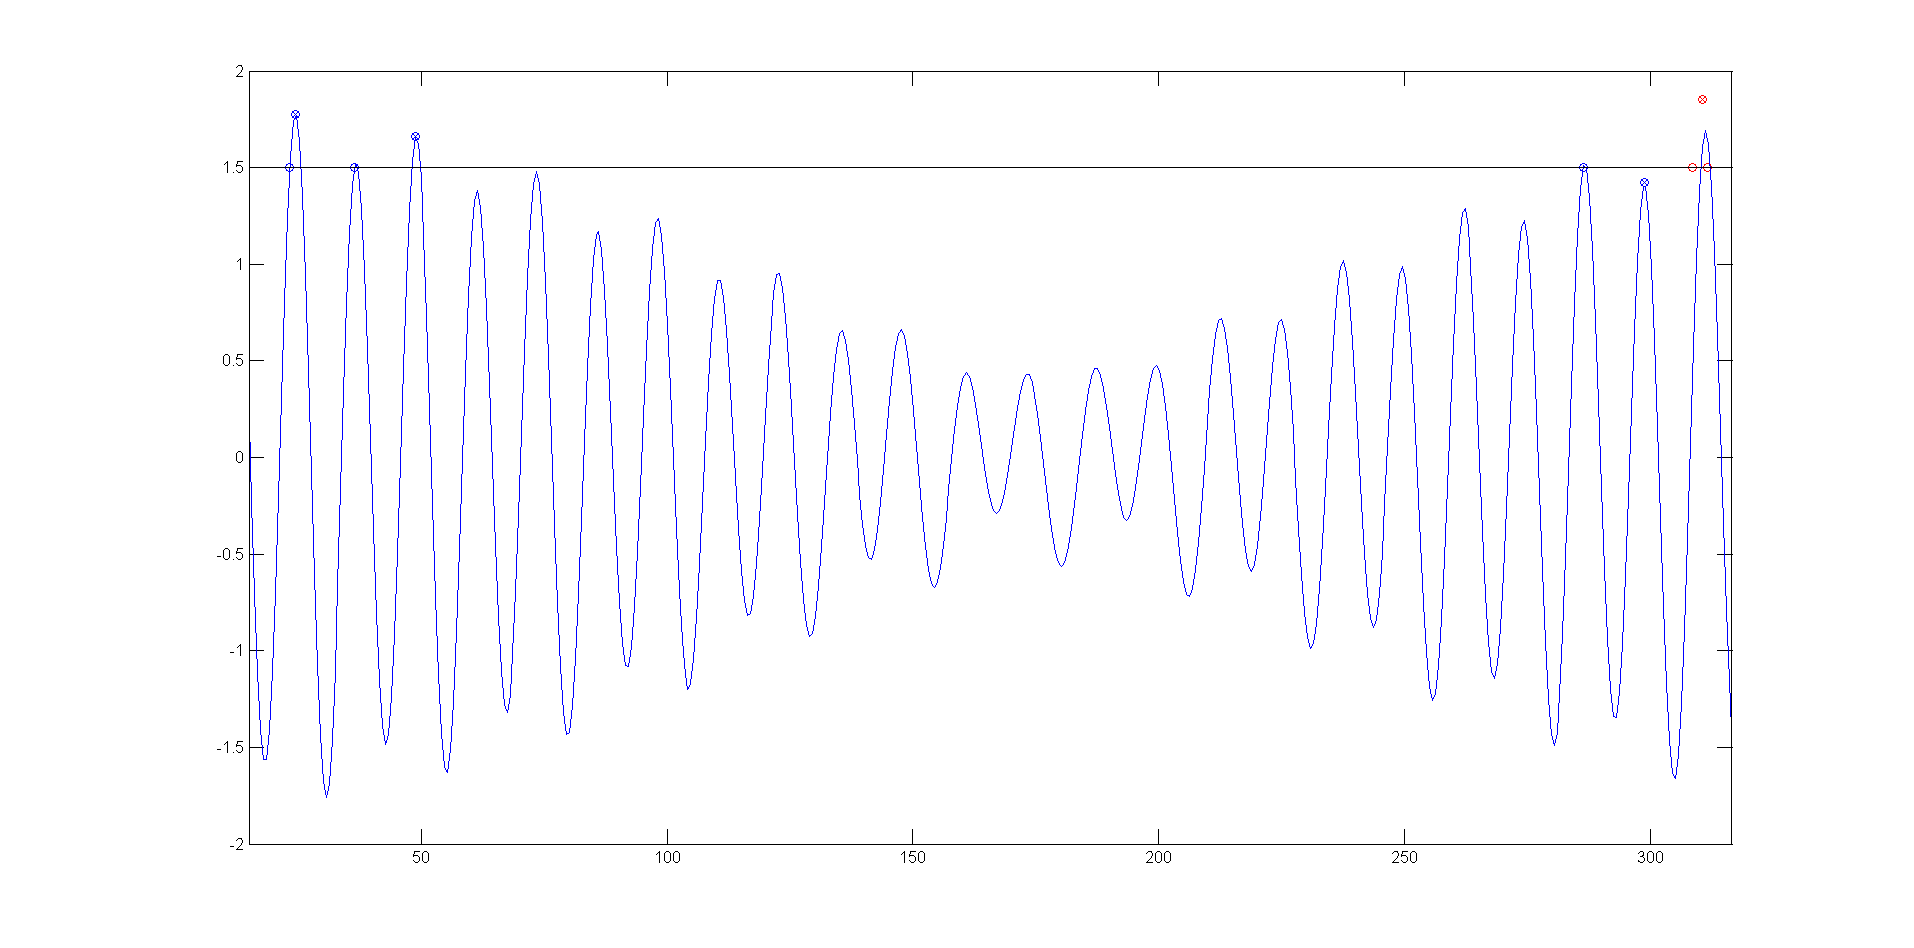
\includegraphics[width=0.5\textwidth]{adapt1_a.png}
	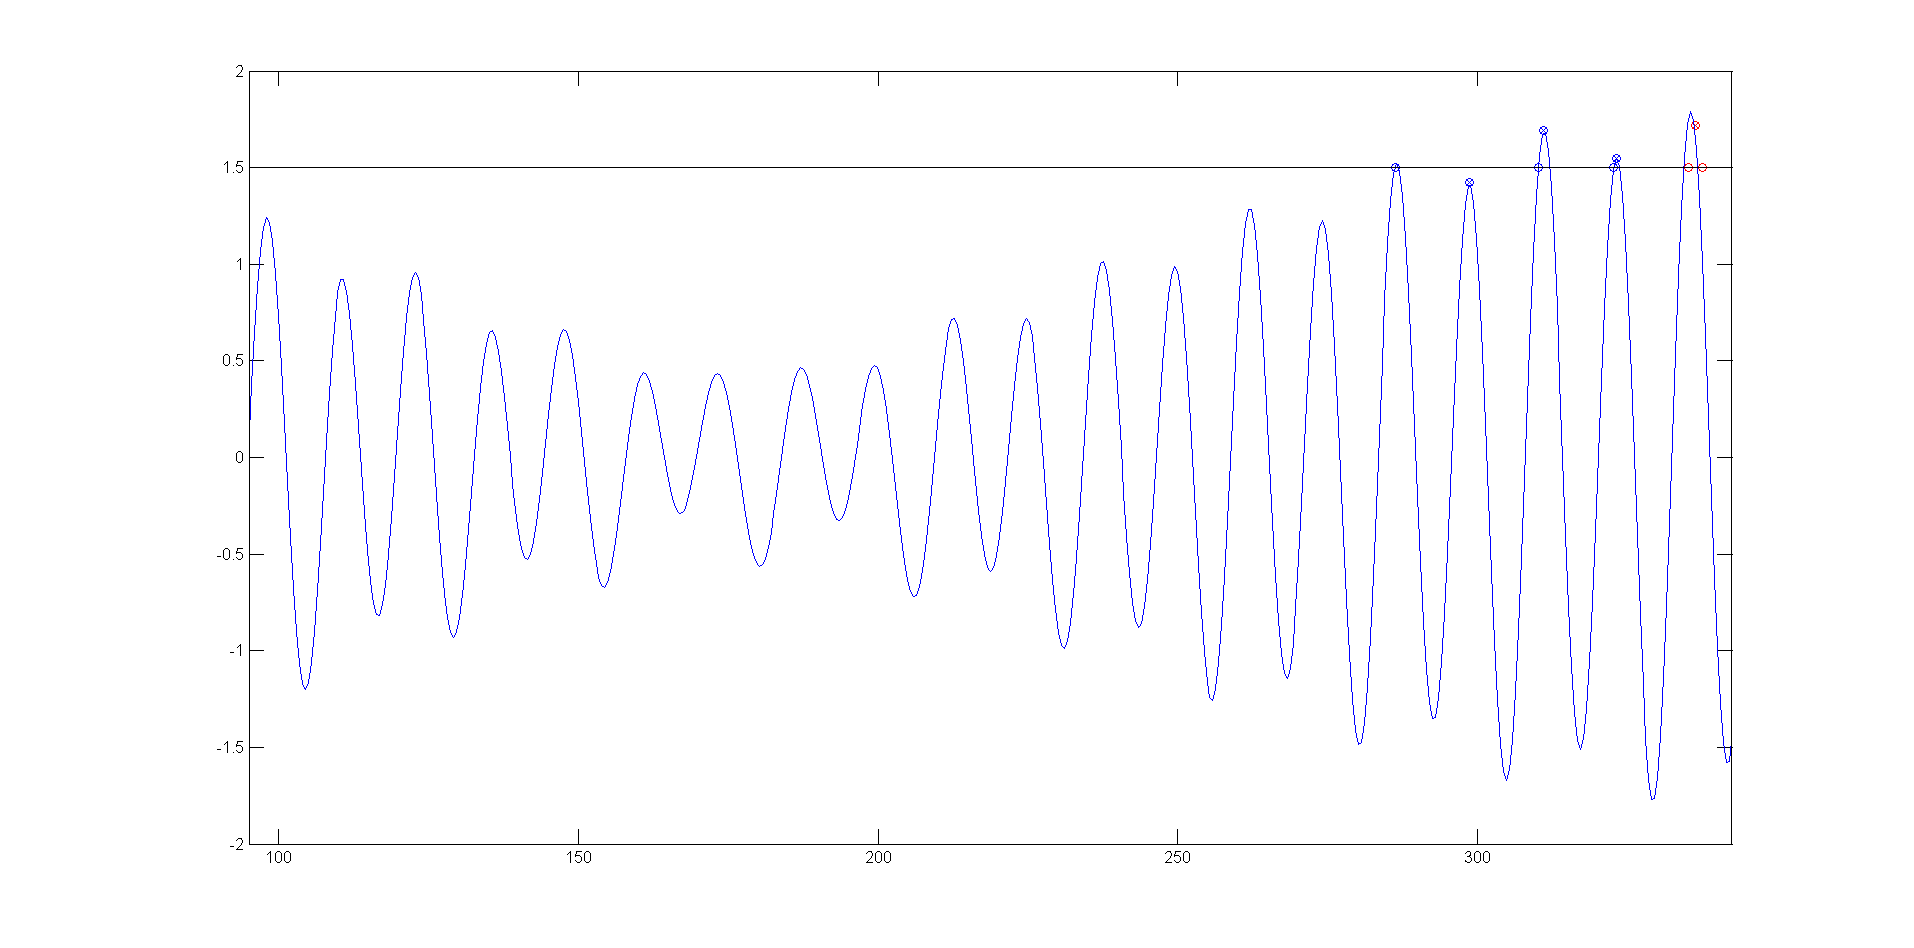
\includegraphics[width=0.5\textwidth]{adapt1_b.png}
	e due previsioni alla nuova altitudine dopo l'addestramento\\
	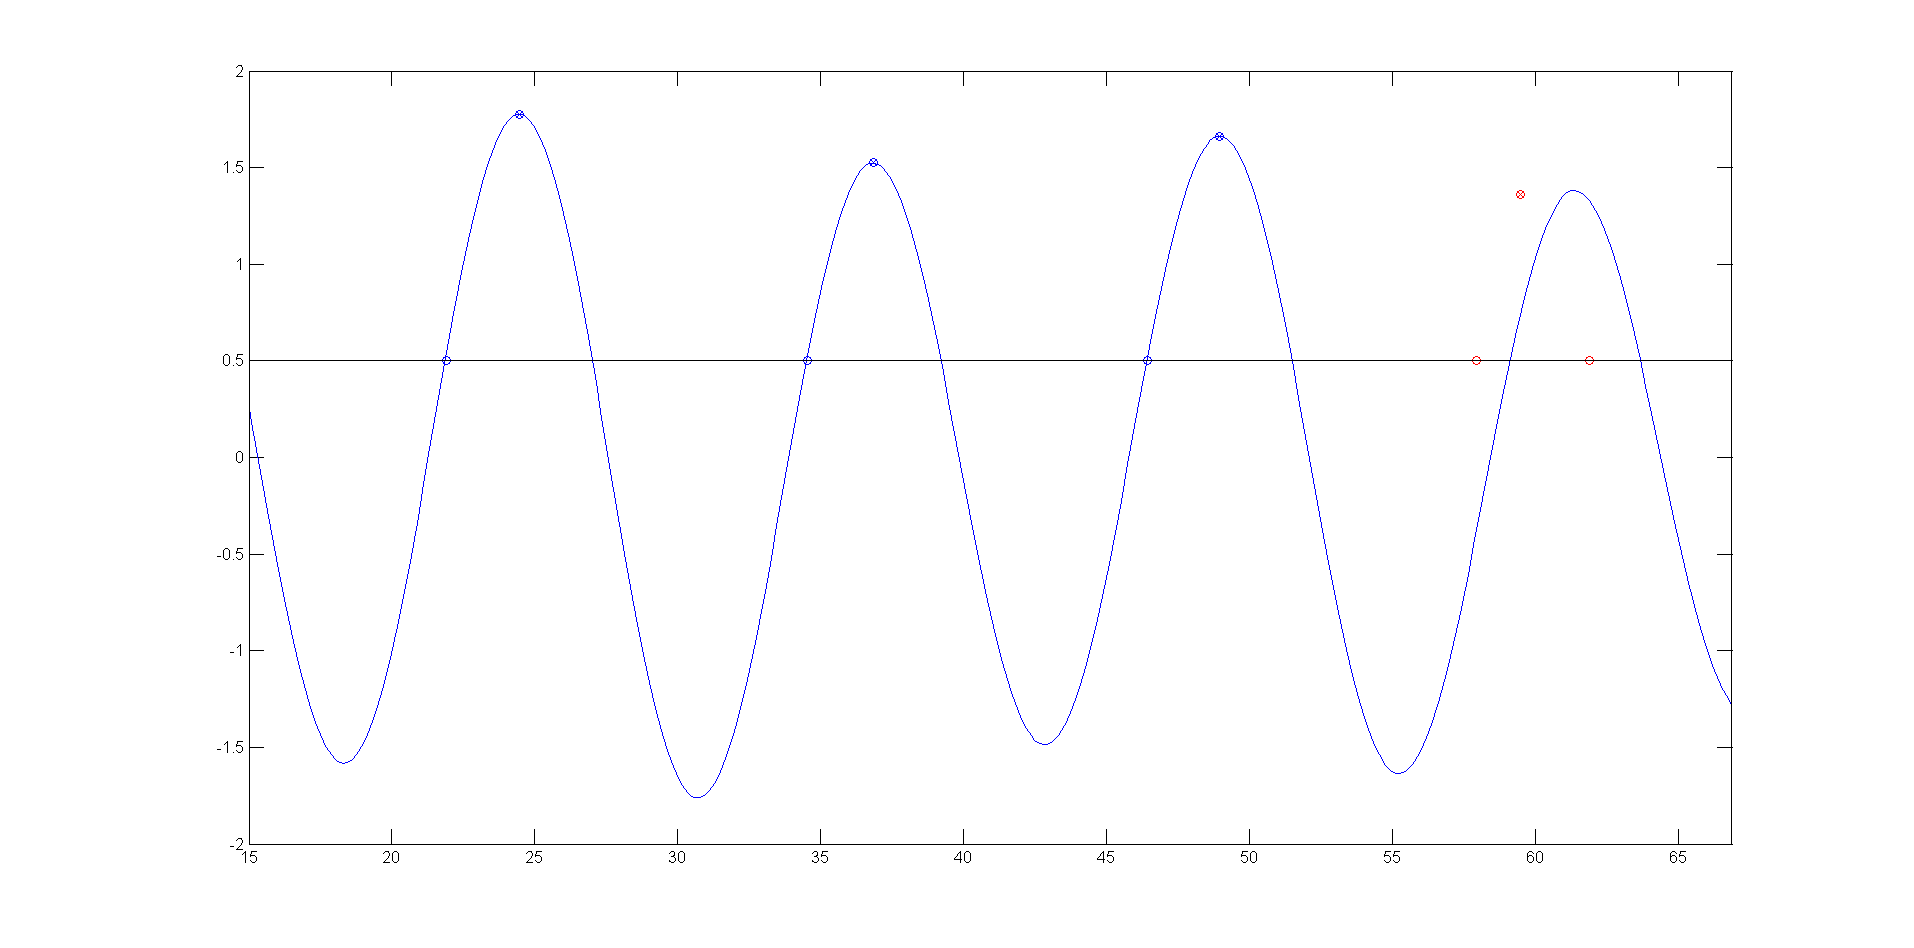
\includegraphics[width=0.5\textwidth]{adapt2_a.png}
	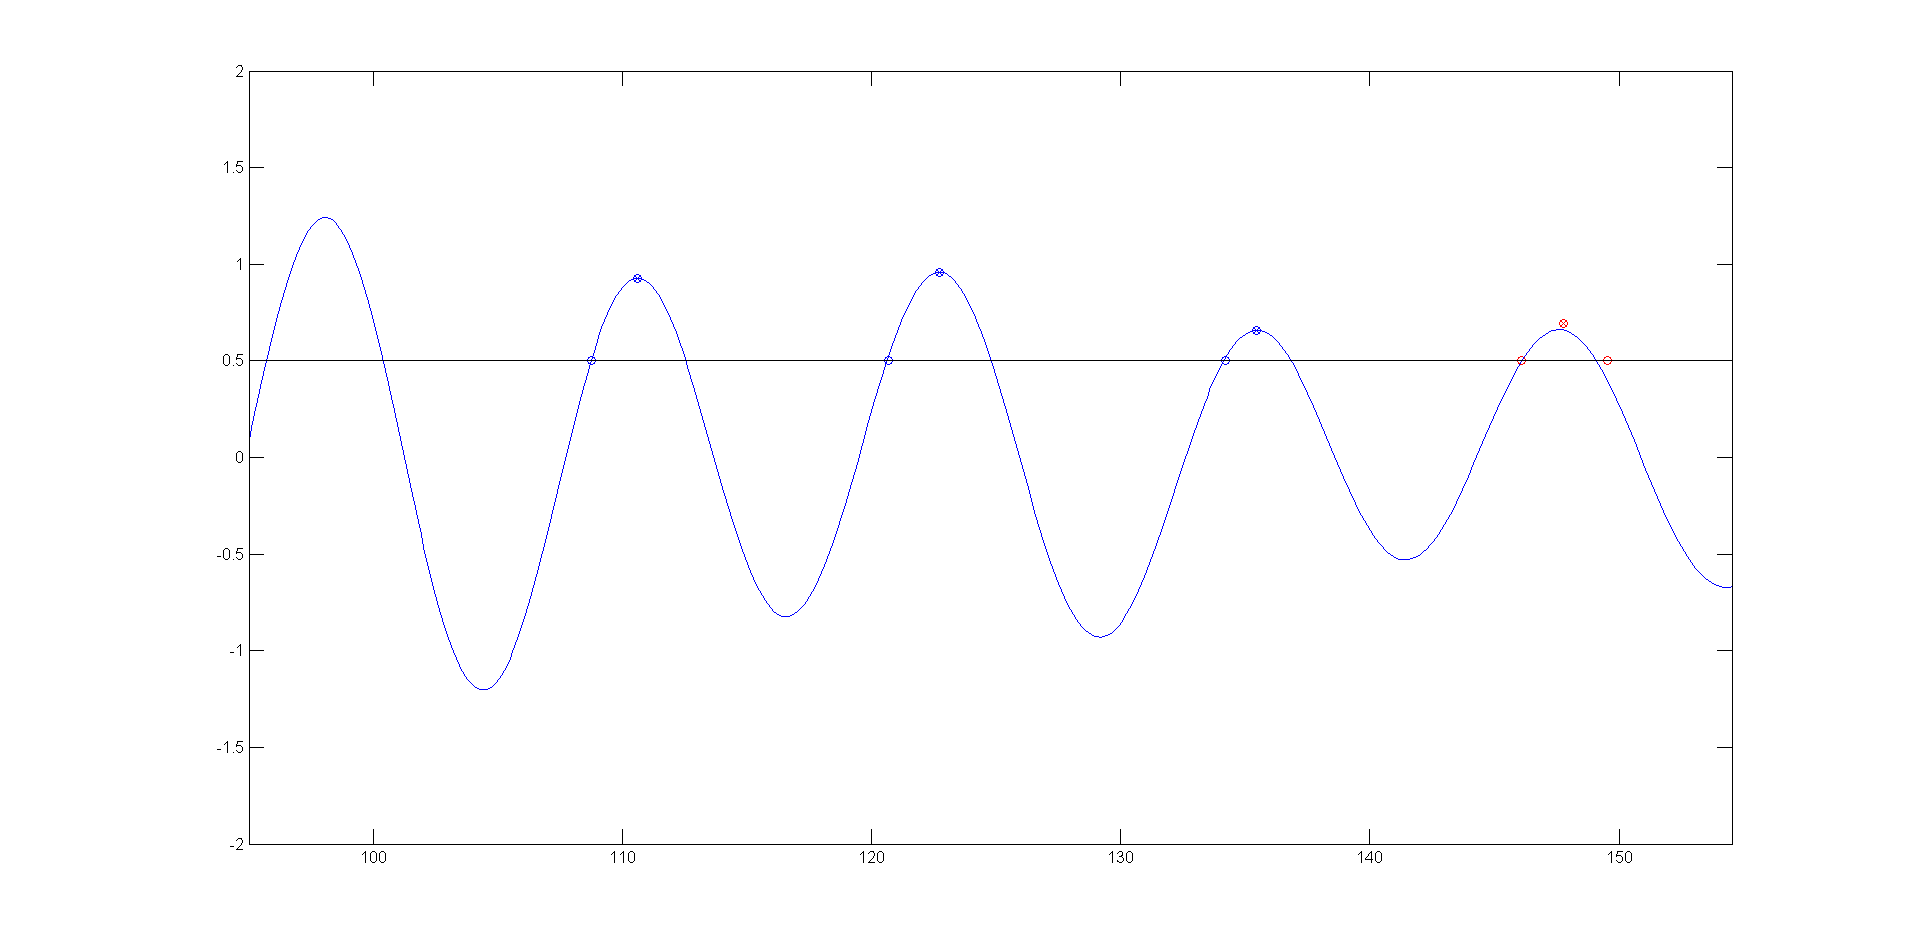
\includegraphics[width=0.5\textwidth]{adapt2_b.png}
	Il Codice \textsc{Matlab} utilizzato per queste simulazioni è il Codice \ref{lst:tideFF_adapt}, Listato del codice.
	
	\chapter*{Listato del codice}
	\addcontentsline{toc}{chapter}{Listato del codice}
	\section*{Capitolo 1}
		\addcontentsline{toc}{section}{Capitolo 1}
		\markboth{\textsc{\Large Listato del codice}}{\textsc{\Large Listato del codice, Capitolo 1}}
		\subsection*{es1\_1.m} \lstinputlisting{code/es1_1.m}
		\subsection*{es1\_4.m} \lstinputlisting{code/es1_4.m}
		\subsection*{es1\_8.m} \lstinputlisting{code/es1_8.m}
		\subsection*{es1\_10.m} \lstinputlisting{code/es1_10.m}
		\subsection*{es1\_11.m} \lstinputlisting{code/es1_11.m}
		\subsection*{es1\_12.m} \lstinputlisting{code/es1_12.m}
		\subsection*{es1\_17.m} \lstinputlisting{code/es1_17.m}
		\subsection*{es1\_18.m} \lstinputlisting{code/es1_18.m}
	\section*{Capitolo 2}
		\addcontentsline{toc}{section}{Capitolo 2}
		\markboth{\textsc{\Large Listato del codice}}{\textsc{\Large Listato del codice, Capitolo 2}}
		\subsection*{newtonSqrt.m} \lstinputlisting{code/newtonSqrt.m}
		\subsection*{es2\_1.m} \lstinputlisting{code/es2_1.m}
		\subsection*{newtonNrt.m} \lstinputlisting{code/newtonNrt.m}
		\subsection*{secantiSqrt.m} \lstinputlisting{code/secantiSqrt.m}
		\subsection*{es2\_3.m} \lstinputlisting{code/es2_3.m}
		\subsection*{newton.m} \lstinputlisting{code/newton.m}
		\subsection*{es2\_4.m} \lstinputlisting{code/es2_4.m}
		\subsection*{newtonMod.m} \lstinputlisting{code/newtonMod.m}
		\subsection*{aitken.m} \lstinputlisting{code/aitken.m}
		\subsection*{es2\_5.m} \lstinputlisting{code/es2_5.m}
		\subsection*{corde.m} \lstinputlisting{code/corde.m}
		\subsection*{secanti.m} \lstinputlisting{code/secanti.m}
		\subsection*{es2\_7.m} \lstinputlisting{code/es2_7.m}
		\subsection*{bisezione.m} \lstinputlisting{code/bisezione.m}
		\subsection*{es2\_8.m} \lstinputlisting{code/es2_8.m}
	\section*{Capitolo 3}
		\addcontentsline{toc}{section}{Capitolo 3}
		\markboth{\textsc{\Large Listato del codice}}{\textsc{\Large Listato del codice, Capitolo 3}}
		\subsection*{triangolareInfRiga.m} \lstinputlisting{code/triangolareInfRiga.m}
		\subsection*{triangolareInfCol.m} \lstinputlisting{code/triangolareInfCol.m}
		\subsection*{triangolareSupRiga.m} \lstinputlisting{code/triangolareSupRiga.m}
		\subsection*{triangolareSupCol.m} \lstinputlisting{code/triangolareSupCol.m}
		\subsection*{fattorizzaLU.m} \lstinputlisting{code/fattorizzaLU.m}
		\subsection*{risolviSistemaLU.m} \lstinputlisting{code/risolviSistemaLU.m}
		\subsection*{fattorizzaLDLt.m} \lstinputlisting{code/fattorizzaLDLt.m}
		\subsection*{risolviSistemaLDLt.m} \lstinputlisting{code/risolviSistemaLDLt.m}
		\subsection*{es3\_18.m} \lstinputlisting{code/es3_18.m}
		\subsection*{fattorizzaLUpivoting.m} \lstinputlisting{code/fattorizzaLUpivoting.m}
		\subsection*{es3\_23.m} \lstinputlisting{code/es3_23.m}
		\subsection*{fattorizzaQR.m} \lstinputlisting{code/fattorizzaQR.m}
		\subsection*{risolviSistemaQR.m} \lstinputlisting{code/risolviSistemaQR.m}
		\subsection*{es3\_31.m} \lstinputlisting{code/es3_31.m}
	\section*{Capitolo 4}
		\addcontentsline{toc}{section}{Capitolo 4}
		\markboth{\textsc{\Large Listato del codice}}{\textsc{\Large Listato del codice, Capitolo 4}}
	\section*{Capitolo 5}
		\addcontentsline{toc}{section}{Capitolo 5}
		\markboth{\textsc{\Large Listato del codice}}{\textsc{\Large Listato del codice, Capitolo 5}}
	\section*{Capitolo 6}
		\addcontentsline{toc}{section}{Capitolo 6}
		\markboth{\textsc{\Large Listato del codice}}{\textsc{\Large Listato del codice, Capitolo 6}}
	
	\nocite{*}
	\bibliographystyle{plainnat}
	\bibliography{bibliography}
	
\end{document}